%%%%%%%%%%%%%%%%%%%%%%%%%%%%%%%%%%%%%%%%%%%%%%%%%%%%%%%%%%%%%%%%%%%%%%%%%%%%%%%%
%%%%%%%%%%%%%%%%%%%%%%%%%%%%%%%%%%%%%%%%%%%%%%%%%%%%%%%%%%%%%%%%%%%%%%%%%%%%%%%%
%%                                                                            %%
%% thesistemplate.tex version 3.20 (2018/08/31)                               %%
%% The LaTeX template file to be used with the aaltothesis.sty (version 3.20) %%
%% style file.                                                                %%
%% This package requires pdfx.sty v. 1.5.84 (2017/05/18) or newer.            %%
%%                                                                            %%
%% This is licensed under the terms of the MIT license below.                 %%
%%                                                                            %%
%% Written by Luis R.J. Costa.                                                %%
%% Currently developed at the Learning Services of Aalto University School of %%
%% Electrical Engineering by Luis R.J. Costa since May 2017.                  %%
%%                                                                            %%
%% Copyright 2017-2018, by Luis R.J. Costa, luis.costa@aalto.fi,              %%
%% Copyright 2017-2018 Swedish translations in aaltothesis.cls by Elisabeth   %%
%% Nyberg, elisabeth.nyberg@aalto.fi and Henrik Wallén,                       %%
%% henrik.wallen@aalto.fi.                                                    %%
%% Copyright 2017-2018 Finnish documentation in the template opinnatepohja.tex%%
%% by Perttu Puska, perttu.puska@aalto.fi, and Luis R.J. Costa.               %%
%% Copyright 2018 English template thesistemplate.tex by Luis R.J. Costa.     %%
%% Copyright 2018 Swedish template kandidatarbetsbotten.tex by Henrik Wallen. %%
%%                                                                            %%
%% Permission is hereby granted, free of charge, to any person obtaining a    %%
%% copy of this software and associated documentation files (the "Software"), %%
%% to deal in the Software without restriction, including without limitation  %%
%% the rights to use, copy, modify, merge, publish, distribute, sublicense,   %%
%% and/or sell copies of the Software, and to permit persons to whom the      %%
%% Software is furnished to do so, subject to the following conditions:       %%
%% The above copyright notice and this permission notice shall be included in %%
%% all copies or substantial portions of the Software.                        %%
%% THE SOFTWARE IS PROVIDED "AS IS", WITHOUT WARRANTY OF ANY KIND, EXPRESS OR %%
%% IMPLIED, INCLUDING BUT NOT LIMITED TO THE WARRANTIES OF MERCHANTABILITY,   %%
%% FITNESS FOR A PARTICULAR PURPOSE AND NONINFRINGEMENT. IN NO EVENT SHALL    %%
%% THE AUTHORS OR COPYRIGHT HOLDERS BE LIABLE FOR ANY CLAIM, DAMAGES OR OTHER %%
%% LIABILITY, WHETHER IN AN ACTION OF CONTRACT, TORT OR OTHERWISE, ARISING    %%
%% FROM, OUT OF OR IN CONNECTION WITH THE SOFTWARE OR THE USE OR OTHER        %%
%% DEALINGS IN THE SOFTWARE.                                                  %%
%%                                                                            %%
%%                                                                            %%
%%%%%%%%%%%%%%%%%%%%%%%%%%%%%%%%%%%%%%%%%%%%%%%%%%%%%%%%%%%%%%%%%%%%%%%%%%%%%%%%
%%                                                                            %%
%%                                                                            %%
%% An example for writting your thesis using LaTeX                            %%
%% Original version and development work by Luis Costa, changes to the text   %% 
%% in the Finnish template by Perttu Puska.                                   %%
%% Support for Swedish added 15092014                                         %%
%% PDF/A-b support added on 15092017                                          %%
%% PDF/A-2 support added on 24042018                                          %%
%%                                                                            %%
%% This example consists of the files                                         %%
%%         thesistemplate.tex (version 3.20) (for text in English)            %%
%%         opinnaytepohja.tex (version 3.20) (for text in Finnish)            %%
%%         kandidatarbetsbotten.tex (version 1.00) (for text in Swedish)      %%
%%         aaltothesis.cls (versio 3.20)                                      %%
%%         kuva1.eps (graphics file)                                          %%
%%         kuva2.eps (graphics file)                                          %%
%%         kuva1.jpg (graphics file)                                          %%
%%         kuva2.jpg (graphics file)                                          %%
%%         kuva1.png (graphics file)                                          %%
%%         kuva2.png (graphics file)                                          %%
%%         kuva1.pdf (graphics file)                                          %%
%%         kuva2.pdf (graphics file)                                          %%
%%                                                                            %%
%%                                                                            %%
%% Typeset in Linux either with                                               %%
%% pdflatex: (recommended method)                                             %%
%%             $ pdflatex thesistemplate                                      %%
%%             $ pdflatex thesistemplate                                      %%
%%                                                                            %%
%%   The result is the file thesistemplate.pdf that is PDF/A compliant, if    %%
%%   you have chosen the proper \documenclass options (see comments below)    %%
%%   and your included graphics files have no problems.
%%                                                                            %%
%% Or                                                                         %%
%% latex: (this method is not recommended)                                    %%
%%             $ latex thesistemplate                                         %%
%%             $ latex thesistemplate                                         %%
%%                                                                            %%
%%   The result is the file thesistemplate.dvi, which is converted to ps      %%
%%   format as follows:                                                       %%
%%                                                                            %%
%%             $ dvips thesistemplate -o                                      %%
%%                                                                            %%
%%   and then to pdf as follows:                                              %%
%%                                                                            %%
%%             $ ps2pdf thesistemplate.ps                                     %%
%%                                                                            %%
%%   This pdf file is not PDF/A compliant. You must must make it so using,    %%
%%   e.g., Acrobat Pro or PDF-XChange.                                        %%
%%                                                                            %%
%%                                                                            %%
%% Explanatory comments in this example begin with the characters %%, and     %%
%% changes that the user can make with the character %                        %%
%%                                                                            %%
%%%%%%%%%%%%%%%%%%%%%%%%%%%%%%%%%%%%%%%%%%%%%%%%%%%%%%%%%%%%%%%%%%%%%%%%%%%%%%%%
%%%%%%%%%%%%%%%%%%%%%%%%%%%%%%%%%%%%%%%%%%%%%%%%%%%%%%%%%%%%%%%%%%%%%%%%%%%%%%%%
%%
%% WHAT is PDF/A
%%
%% PDF/A is the ISO-standardized version of the pdf. The standard's goal is to
%% ensure that he file is reproducable even after a long time. PDF/A differs
%% from pdf in that it allows only those pdf features that support long-term
%% archiving of a file. For example, PDF/A requires that all used fonts are
%% embedded in the file, whereas a normal pdf can contain only a link to the
%% fonts in the system of the reader of the file. PDF/A also requires, among
%% other things, data on colour definition and the encryption used.
%% Currently three PDF/A standards exist:
%% PDF/A-1: based on PDF 1.4, standard ISO19005-1, published in 2005.
%%          Includes all the requirements essential for long-term archiving.
%% PDF/A-2: based on PDF 1.7, standard ISO19005-2, published in 2011.
%%          In addition to the above, it supports embedding of OpenType fonts,
%%          transparency in the colour definition and digital signatures.
%% PDF/A-3: based on PDF 1.7, standard ISO19005-3, published in 2012.
%%          Differs from the above only in that it allows embedding of files in
%%          any format (e.g., xml, csv, cad, spreadsheet or wordprocessing
%%          formats) into the pdf file.
%% PDF/A-1 files are not necessarily PDF/A-2 -compatible and PDF/A-2 are not
%% necessarily PDF/A-1 -compatible.
%% All of the above PDF/A standards have two levels:
%% b: (basic) requires that the visual appearance of the document is reliably
%%    reproduceable.
%% a (accessible) in addition to the b-level requirements, specifies how
%%   accessible the pdf file is to assistive software, say, for the physically
%%   impaired.
%% For more details on PDF/A, see, e.g., https://en.wikipedia.org/wiki/PDF/A
%%
%%
%% WHICH PDF/A standard should my thesis conform to?
%%
%% Primarily to the PDF/A-1b standard. All the figures and graphs typically
%% use in thesis work do not require transparency features, a basic '2-D'
%% visualisation suffices. The font to be used are specified in this template
%% and they should not be changed. However, if you have figures where
%% transparency characteristics matter, use the PDF/A-2b standard. Do not use
%% the PDF/A-3b standard for your thesis.
%%
%%
%% WHAT graphics format can I use to produce my PDF/A compliant file?
%%
%% When using pdflatex to compile your work, use jpg, png or pdf files. You may
%% have PDF/A compliance problems with figures in pdf format. Do not use PDF/A
%% compliant graphics files.
%% If you decide to use latex to compile your work, the only acceptable file
%% format for your figure is eps. DO NOT use the ps format for your figures.

%% USE one of these:
%% * the first when using pdflatex, which directly typesets your document in the
%%   chosen pdf/a format and you want to publish your thesis online,

%% * the second when you want to print your thesis to bind it, or
%% * the third when producing a ps file and a pdf/a from it.
%%
\documentclass[english, 12pt, a4paper, elec, utf8, a-1b, online]{aaltothesis}
%\documentclass[english, 12pt, a4paper, elec, utf8, a-1b]{aaltothesis}
%\documentclass[english, 12pt, a4paper, elec, dvips, online]{aaltothesis}

%% Use the following options in the \documentclass macro above:
%% your school: arts, biz, chem, elec, eng, sci
%% the character encoding scheme used by your editor: utf8, latin1
%% thesis language: english, finnish, swedish
%% make an archiveable PDF/A-1b or PDF/A-2b compliant file: a-1b, a-2b
%%                    (with pdflatex, a normal pdf containing metadata is
%%                     produced without the a-*b option)
%% typeset in symmetric layout and blue hypertext for online publication: online
%%            (no option is the default, resulting in a wide margin on the
%%             binding side of the page and black hypertext)
%% two-sided printing: twoside (default is one-sided printing)
%%

%% Use one of these if you write in Finnish (see the Finnish template
%% opinnaytepohja.tex)
%\documentclass[finnish, 12pt, a4paper, elec, utf8, a-1b, online]{aaltothesis}
%\documentclass[finnish, 12pt, a4paper, elec, utf8, a-1b]{aaltothesis}
%\documentclass[finnish, 12pt, a4paper, elec, dvips, online]{aaltothesis}

%% Commands
\newcommand{\shellcmd}[1]{\fcolorbox{lightgray}{lightgray}{#1}}

%% Packages
\usepackage{graphicx}
%% Graphics path
\graphicspath{{doc/0_figures/}}

%% Math fonts, symbols, and formatting; these are usually needed
\usepackage{amsfonts,amssymb,amsbsy,amsmath,gensymb}
\usepackage{wasysym}

%% Glossaries and acronyms
\usepackage[xindy,acronym,nomain,nopostdot,nogroupskip,nonumberlist,acronymlists={acronym,symbolslist,operatorslist}]{glossaries}
\newglossary[tlg]{symbolslist}{tld}{tdn}{Symbols}
\newglossary[slg]{operatorslist}{syi}{syg}{Operators}
\makenoidxglossaries
\loadglsentries{97_glossary}
\glsaddall
\setlength{\glsdescwidth}{0.88\hsize}
\setglossarysection{subsection}

%% Bibliography
\usepackage[backend=biber,citestyle=ieee,citestyle=numeric-comp]{biblatex}
\usepackage{csquotes}
\addbibresource{doc/thesis/99_references.bib}

\usepackage[binary-units=true]{siunitx}
\usepackage{float}
\usepackage{caption}
\usepackage{subcaption}
\usepackage{tabularx}
\usepackage{colortbl}

\usepackage{dirtree}

%% Change the school field to specify your school if the automatically set name
%% is wrong
% \university{aalto-yliopisto}
% \school{Sähkötekniikan korkeakoulu}

%% Edit to conform to your degree programme
%%
\degreeprogram{Space Science and Technology}
%%

%% Your major
%%
\major{Space Robotics and Automation}
%%

%% Major subject code
%%
\code{ELEC3047}
%%
 
%% Choose one of the three below
%%
%\univdegree{BSc}
\univdegree{MSc}
%\univdegree{Lic}
%%

%% Your name (self explanatory...)
%%
\thesisauthor{Gabriel J\"org Schwarzkopf}
%%

%% Your thesis title comes here and possibly again together with the Finnish or
%% Swedish abstract. Do not hyphenate the title, and avoid writing too long a
%% title. Should LaTeX typeset a long title unsatisfactorily, you mght have to
%% force a linebreak using the \\ control characters.
%% In this case...
%% Remember, the title should not be hyphenated!
%% A possible "and" in the title should not be the last word in the line, it
%% begins the next line.
%% Specify the title again without the linebreak characters in the optional
%% argument in box brackets. This is done because the title is part of the 
%% metadata in the pdf/a file, and the metadata cannot contain linebreaks.
%%
\thesistitle{3D Reconstruction of small Solar System bodies using rendered and compressed images}
%\thesistitle[Title of the thesis]{Title of\\ the thesis}
%% Near-target navigation and mass determination using optical reconstruction of small solar system bodies
%% 

%%
\place{Espoo}
%%

%% The date for the bachelor's thesis is the day it is presented
%%
\date{24.2.2020}
%%

%% Thesis supervisor
%% Note the "\" character in the title after the period and before the space
%% and the following character string.
%% This is because the period is not the end of a sentence after which a
%% slightly longer space follows, but what is desired is a regular interword
%% space.
%%
\supervisor{Prof.\ Jaan Praks}
%%

%% Advisor(s)---two at the most---of the thesis. Check with your supervisor how
%% many official advisors you can have.
%%
\advisor{Dr.\ Andris Slavinskis}
%\advisor{MSc Sarah Scientist}
%%

%% Aaltologo: syntax:
%% \uselogo{aaltoRed|aaltoBlue|aaltoYellow|aaltoGray|aaltoGrayScale}{?|!|''}
%% The logo language is set to be the same as the thesis language.
%%
\uselogo{aaltoRed}{''}
%%

%% The English abstract:
%% All the details (name, title, etc.) on the abstract page appear as specified
%% above.
%% Thesis keywords:
%% Note! The keywords are separated using the \spc macro
%%
\keywords{Deep Space\spc Simulation\spc Small Solar System Bodies\spc Compression\spc Rendering\spc Reconstruction}
%%

%% The abstract text. This text is included in the metadata of the pdf file as well
%% as the abstract page.
%%
\thesisabstract{
Synthetic image generation and reconstruction of small Solar System bodies and the influence of compression is becoming an important topic to study because of the advent of using small spacecraft in deep space missions. Most of these missions will use fly-by scenarios, for example in the Comet Interceptor mission. Due to limited data budgets, maximising the scientific output of small satellites requires investigating effects of lossy compression. We have developed a simulation environment that uses physics-based rendering in combination with procedural terrain generation to overcome limitations of currently used methods for image rendering like the Hapke model. The rendered small Solar System body images are combined with a star background and photometrically calibrated to represent realistic images. We implemented a Structure-from-Motion pipeline to reconstruct three-dimensional models from the rendered images. In this work, we developed a compression software package to investigate effects of lossy compression on reconstructed models and the possible amount of data reduction of lossy compression to lossless compression. Several scenarios with varying fly-by distances ranging from 50 km to 400 km and body sizes of 1 km and 10 km were simulated and compressed with lossless and several quality levels of lossy compression using JPEG 2000. We have found that low compression ratios introduce changes resembling random noise while high compression ratios remove surface features. We found that the random noise artefacts introduced by low compression ratios can increase the number of vertices and faces of the reconstructed three-dimensional model. 
}

% Your abstract in English. Keep the abstract short. The abstract explains your 
% research topic, the methods you have used, and the results you obtained. In the 
% PDF/A format of this thesis, in addition to the abstract page, the abstract text is 
% written into the pdf file's metadata. Write here the text that goes into the 
% metadata. The metadata cannot contain special characters, linebreak or paragraph 
% break characters, so these must not be used here. If your abstract does not contain 
% special characters and it does not require paragraphs, you may take advantage of 
% the abstracttext macro (see the comment below). Otherwise, the metadata abstract 
% text must be identical to the text on the abstract page.

%% Copyright text. Copyright of a work is with the creator/author of the work
%% regardless of whether the copyright mark is explicitly in the work or not.
%% You may, if you wish, publish your work under a Creative Commons license (see
%% creaticecommons.org), in which case the license text must be visible in the
%% work. Write here the copyright text you want. It is written into the metadata
%% of the pdf file as well.
%% Syntax:
%% \copyrigthtext{metadata text}{text visible on the page}
%% 
%% In the macro below, the text written in the metadata must have a \noexpand
%% macro before the \copyright special character, and macros (\copyright and
%% \year here) must be separated by the \ character (space chacter) from the
%% text that follows. The macros in the argument of the \copyrighttext macro
%% automatically insert the year and the author's name. (Note! \ThesisAuthor is
%% an internal macro of the aaltothesis.cls class file).
%% Of course, the same text could have simply been written as
%% \copyrighttext{Copyright \noexpand\copyright\ 2018 Eddie Engineer}
%% {Copyright \copyright{} 2018 Eddie Engineer}
%%
\copyrighttext{Copyright \noexpand\copyright\ \number\year\ \ThesisAuthor}
{Copyright \copyright{} \number\year{} \ThesisAuthor}

%% You can prevent LaTeX from writing into the xmpdata file (it contains all the 
%% metadata to be written into the pdf file) by setting the writexmpdata switch
%% to 'false'. This allows you to write the metadata in the correct format
%% directly into the file thesistemplate.xmpdata.
%\setboolean{writexmpdatafile}{false}



%% All that is printed on paper starts here
%%
\begin{document}

%% Create the coverpage
%%
\makecoverpage

%% Typeset the copyright text.
%% If you wish, you may leave out the copyright text from the human-readable
%% page of the pdf file. This may seem like a attractive idea for the printed
%% document especially if "Copyright (c) yyyy Eddie Engineer" is the only text
%% on the page. However, the recommendation is to print this copyright text.
%%
\makecopyrightpage

%% Note that when writting your thesis in English, place the English abstract
%% first followed by the possible Finnish or Swedish abstract.

%% Abstract text
%% All the details (name, title, etc.) on the abstract page appear as specified
%% above.
%%
% \begin{abstractpage}[english]
%   Your abstract in English. Keep the abstract short. The abstract explains your
%   research topic, the methods you have used, and the results you obtained.  
  
%   The abstract text of this thesis is written on the readable abstract page as
%   well as into the pdf file's metadata via the $\backslash$thesisabstract macro
%   (see above). Write here the text that goes onto the readable abstract page.
%   You can have special characters, linebreaks, and paragraphs here. Otherwise,
%   this abstract text must be identical to the metadata abstract text.
  
%   If your abstract does not contain special characters and it does not require
%   paragraphs, you may take advantage of the abstracttext macro (see the comment
%   below).
% \end{abstractpage}

%% The text in the \thesisabstract macro is stored in the macro \abstractext, so
%% you can use the text metadata abstract directly as follows:
%%
\begin{abstractpage}[english]
	\abstracttext{}
\end{abstractpage}

%% Preface
%%
%% This section is optional. Remove it if you do not want a preface.
\mysection{Preface}
%\mysection{Esipuhe}
I want to thank Professor Jaan Praks and my instructor Andris Slavinskis, PhD for 
their good and poor guidance.\\

\vspace{5cm}
Otaniemi, 23.2.2020

\vspace{5mm}
{\hfill \ThesisAuthor \hspace{1cm}}

%% Force a new page after the preface
%%
\newpage


%% Table of contents. 
%%
\thesistableofcontents


%% Symbols and abbreviations
\mysection{Symbols and abbreviations}

\printnoidxglossary[type=symbolslist, style=long]

\printnoidxglossary[type=operatorslist, style=long]

\printnoidxglossary[type=\acronymtype, style=long, title={Abbreviations}] 

%% \clearpage is similar to \newpage, but it also flushes the floats (figures
%% and tables).
%%
\cleardoublepage

%% Text body begins. Note that since the text body is mostly in Finnish the
%% majority of comments are also in Finnish after this point. There is no point
%% in explaining Finnish-language specific thesis conventions in English.
%% This text will be translated to English soon.
%%


%% Leave page number of the first page empty
%% 
\thispagestyle{empty}


%% In a thesis, every section starts a new page, hence \clearpage
\clearpage
\section{Introduction} \label{sec:introduction}
%Deep Space Missions
%-science (planetary defence)
%    -navigation autonomy
%    -maximising science output
%        -high risk environments
%        -small data budgets
%            -compression
%    -CI
%        -unknown object, small real image database
%-economy
%    -navigation autonomy
%    -knowledge about composition, size and shape -> science
%==> autonomy, max sci, unknown object -> synthetic image generation, compression and reconstruction -> sispo covers all three topics

%SSSBs visited: Ryugu, Bennu, Ceres, C-G, Vesta, Tempel 1, Hartley, Lutetia, Itokava, Steins, Wild 2, Annefrank, Borrelly, Eros, Braille, Mathilde, Ida, Gaspra, Halley, Giacobini-Zinner

The study of \gls{sssb} provides a unique opportunity to understand the evaluation of the Solar System since they are unaltered remnants of the formation phase~\cite{walsh2018rubble, a2017comets}. Rapidly developing technology provides more opportunities to study such objects since interplanetary missions become feasible at a reasonable cost using small spacecraft (\cite{poghosyan2017cubesat}, \cite{andrews2019asteroid}, \cite{snodgrass2019europeanCI}).
In addition, asteroids are becoming interesting to companies -- numerous studies show that asteroid mining can become a viable business in the near future (\cite{andrews2015defining}, \cite{busch2004profitable}, \cite{weinzierl2018EconomicFrontier}, \cite{pittman2017deep}). Several companies, such as Planetary Resources \cite{lewicki2013planetary} or the Asteroid Mining Corporation Ltd. \cite{asteroidminingcorporation} were founded for creating an asteroid mining based business.

A total of \SI{3607}{} comets and \SI{931905}{} asteroids are known as of February 2020 \cite{nasaSBD_count}. Most knowledge about their size, shape and colour is inferred from ground based observations and space telescopes \cite{bowles2018castaway}. Approximately \SI{25}{} of such objects have been visited by spacecraft (\cite{wikipediaVisitedList}, \cite{nasaSBD_missions}). Considering the total of \SI{935512}{} known objects shows the potential number of remaining targets. Several missions to \gls{sssb} are planned. For example, the \textit{Comet Interceptor} mission by \gls{esa} \cite{snodgrass2019europeanCI}, the \textit{HERA} mission by \gls{esa} \cite{hera},  and the \textit{DART} mission by \gls{nasa} \cite{talbert_2017DART}. Closer studies through flyby or orbiting an \gls{sssb} provides more detailed information such as precise size and shape measurements as well as local variations in albedo for example.

Using small and low-cost spacecraft, it becomes possible not only to have more spacecraft to study \gls{sssb}s but also to fly closer to their nuclei, which is scientifically more interesting but associated with a higher risk of losing a spacecraft. This puts two major constraints onto their data budget. Their radio links provide lower data rates and the possibility of losing the spacecraft means transmitting the most important data first and complementing it later, if possible. A  common practice to reduce the amount of data that needs to be transmitted is compression. Therefore it is necessary to investigate the effect of compression, especially on image data. In addition, an algorithm is necessary that can prioritise which data needs to be transmitted first and which can be transmitted later.

All these endeavours lead to an increased number of spacecraft that operate in deep space. Current operations and navigation of spacecraft in deep space relies on \gls{dsn}. Radio signals are used to determine a spacecraft's state vector through ranging and Doppler measurements \cite{ramamurthy2015delta}. Relying on such an infrastructure limits the number of spacecraft that can be operating in deep space. Additionally, this poses not only a risk to a mission due to reliance on a working ground segment, but is also associated with high costs. High costs are especially relevant to small spacecraft mission, since using a \gls{dsn} would increase the overall mission cost substantially \cite{steffes2017deep}. Furthermore, when a spacecraft is obstructed by the Sun, it is not possible to communicate with it and therefore not possible to use such techniques \cite{kominato2006optical}. Another problem with \gls{dsn}-based navigation become apparent with \textit{Comet Interceptor}, where high relative speeds do not allow for long delays associated with ground contacts in deep space. Similarly, with rendez-vous and landing missions to \gls{sssb}s, autonomous orbit determination is essential because mission events are happening too fast for relying on ground interaction \cite{shuang2013imageprocessing}. An alternative to using a \gls{dsn} are \gls{dsan} technologies. \gls{dsan} comprises trajectory and attitude determination only from on-board data and with on-board available computational power. In a next step, this information would be fed into an \gls{aocs} to correct pointing and trajectory errors. For example, optical navigation can be conducted on-board the spacecraft thus eliminating the requirement of ground contact. Optical navigation was already used in the \textit{Deep Space 1} mission cruise phase (\cite{Riedel2000AutonomousReport}, \cite{bhaskaran2012autonomous}). However, autonomous relative optical navigation in the proximity of a Solar System body will be essential for future deep space exploration and space mining economy (\cite{steffes2017deep}, \cite{martin2006jpl}, \cite{probst2016mission}). Hybrid optical navigation was used in the \textit{Hayabusa} mission in the proximity of the asteroid Itokawa. However, this method still relied on radiometric data from the ground segment \cite{kominato2006optical}. Therefore, fully autonomous navigation systems still need to be developed.

For developing navigation algorithms and methods to maximise scientific output, it is necessary to have images of \gls{sssb}s in order to test and validate these algorithms and methods. Although data sets from the \textit{OSIRIS} instrument aboard \textit{Rosetta} \cite{osirisArchive} or from the \textit{OSIRIS-REx}, \textit{Dawn} and \textit{NEAR} missions \cite{palmer2014small} are publicly available, the total number of images and their variation remains small.

Increased spacecraft autonomy around \gls{sssb}, maximising the science output and targeting unknown objects require images from a variety of differing objects to develop systems and algorithms. Since there is only a limited number of real images it is necessary to synthetically create images of \gls{sssb}s. Synthetically creating images of \gls{sssb}s is currently based on the parametric empirical models for directional reflectance properties of airless regolith surfaces, developed by Hapke \cite{hapke1981bidirectional, hapke1981bidirectional2, hapke1984bidirectional, hapke1986bidirectional, hapke2002bidirectional, hapke2008bidirectional, hapke2012bidirectional}. However, the Hapke model is also being challenged because it is an empirical, and not physical, model and because of its shortcomings in some areas \cite{shkuratov2012critical}. One of these areas are shadows, especially at slopes of e.g. craters \cite{shkuratov2012critical}. These are especially relevant to surface features of \gls{sssb}s. One possible solution is to use physics-based rendering with Path-tracing techniques (\cite{shkuratov2012critical}, \cite{lafortune1996mathematical}).

In this thesis, the first implementation of \gls{sispo} is developed. The aim was not to complete development of the software package but to provide a first draft. The implementation covers the entire processing pipeline from rendering and compression to reconstruction of a 3D model. These sub components are combined to form \gls{sispo}. To create realistic observation geometries, trajectories are simulated with proper orbital dynamics in the solar system.

The software package should provide a possibility to simulate different trajectories. Rendering should provide as realistic output as possible. Furthermore, it is necessary to include rendering of various \gls{sssb}s, including different size, shape and surface features. To assess the quality of rendered images and to investigate the impact of compression, it is posited that the quality recovered by an \gls{sfm} pipeline provides a quality measure in the form of the number of reconstructed points, number of vertices and number of faces. \gls{sispo} is being developed to provide these functionalities in a single software package.

%Advancing the field requires improving the statistics on the different types of \gls{sssb}s \cite{Pajusalu2019CharacterizationMapping}. Several new mission ideas are aiming for this goal. However, technological challenges have to be overcome first. Additionally, new mission concepts like the \gls{ci} mission require a new approach to model \gls{sssb}s. \gls{ci} is a mission that will investigate either a dynamically new comet from the Öpik-Oort cloud or an interstellar object. The mission will consist of a main spacecraft and two sub-spacecrafts that will be launched to the \gls{l2} and wait until a suitable \gls{sssb} will pass by. Consequently, the target body will not be known before launch hence systems have to be developed to deal with a large variety of bodies. However, only few \gls{sssb}s have been visited by spacecraft and thus only very limited real images are available. A method to deal with such sparse available data is to synthetically create images of \gls{sssb}s.


%This thesis focuses on image compression and decompression. These effects will be quantified using the reconstructed 3D models against the "ideal" model. A reference instrument definition similar to a suggested instrument for the 'Comet Interceptor' mission. Different compression and decompression algorithms will be evaluated using different \gls{sssb}s. Furthermore, different spacecraft trajectories will be examined to investigate limitations of the simulation environment.


\clearpage
\section{Theory} \label{sec:theory}
% Physics part
% - Composition (photometry) -> telescope optics?/instrument?/bit depth?
% - Trajectories and relative trajectory of spacecraft, especially trajectories for flybys
% - Star rendering?
% - Describe physics of SSSBs, i.e. size/shapes/surface (features/color/albedo) illumination
%
% Computer Science part
% - Physics-based rendering? -Shaders/procedural terrain generation
% - Compression
% - Reconstruction (SfM), relates to camera physics. Generally Computer Vision topic.
% - Image processing Gaussian filtering, downscale local means
% - Logic for choosing number of reconstructed points as quality measure
%
% Space
% - Small Spacecrafts -> small data budgets?
%
% Max Science?
%
% Concepts to describe???

\subsection{Small Solar System Bodies}
The \gls{iau} defines an \gls{sssb} as any object in the Solar System, that is not a planet, dwarf planet or satellite~\cite{iau_sssb}. Within this work, the term \gls{sssb} mostly refers to asteroids and comets.

In a classical definition, asteroids and comets were two distinct \glspl{sssb} classes based on observational, physical and dynamical properties. However, the discovery of active asteroids and dormant comets began to blur these definitions. Many observed objects cannot be strictly classified into the classical categories anymore therefore these objects are more frequently described as part of an asteroid-comet continuum with asteroids and comets at the ends of the continuum~\cite{Hsieh2017Asteroid-cometSystem}.

Despite the shift towards a continuum definition, we use the more classical definition in this work to refer to non-active objects as asteroid and active objects as comets where it is necessary to distinguish between these types of objects. Therefore, a description for the classical definition of asteroids and comets is provided.

\subsubsection{Asteroids}
Asteroids are rocky bodies that mostly reside in an orbit between Mars and Jupiter, i.e. the asteroid main belt. More than \SI{930000}{} asteroids are known of which more than \SI{540000}{} are numbered. The ephemeris of most ($> \SI{930000}{}$ and absolute magnitude of more than \SI{925000}{} is known. However, physical parameters like diameter ($> \SI{136000}{}$), albedo ($> \SI{135000}{}$), rotation period ($> \SI{19000}{}$), spectral type ($> \SI{2000}{}$) and the standard gravitational parameter ($> \SI{10}{}$) are known for only a few objects~\cite{JPLEngine}.

Asteroids are often referred to as rubble piles, i.e. objects which aggregated boulders by gravity giving them a low bulk density because of many void spaces in there internal structure~\cite{Richardson2002GravitationalEvolution}. An example of rubble pile asteroids are Bennu and Ryugu due to their low density~\cite{Chesley2014OrbitBennu, Watanabe2019Hayabusa2Pile}.

\subsubsection{Comets}
Comets are small icy bodies that mostly reside farther away from the Sun than asteroids. Inside the heliosphere, the source of comets is the Kuiper belt while comets from outside the heliosphere are thought to originate in the \"Opik-Oort cloud. Comets are occasionally perturbed by the gravity of other objects which moves their orbits closer to the Sun. While being close to the Sun, volatiles begin to evaporate which creates the well-known coma around the nucleus. In most cases the coma is several orders of magnitudes larger than the nucleus. Nuclei are on the order of a few kilometres while comas can be on the order of hundreds of thousands of kilometres. Additionally, a gas and a dust tail are formed. The gas tail originates from coma charged particles that are carried away from the nucleus by the magnetic field carried by the solar wind. On the other hand, the dust tail is formed by small dust particles in the coma which are carried away from the nucleus by the solar radiation pressure. Larger dust particles remain along a comets trajectory as a trail forming part of the meteoroid environment. If a comet is heated unevenly, trapped gas escapes at weak spots in the surface forming jets of gas and dust~\cite{Comets, a2017comets, Soja2019IMEM2:System}.

The physical parameters of comets are not well known, since they are small and it is difficult to image the nucleus when they come closer to the Sun since the nucleus is surrounded by the coma. Approximately \SI{3500}{} comets are known of which more than \SI{400}{} are numbered~\cite{JPLEngine}. While the ephemeris ($> \SI{1700}{}$) and magnitude ($>\SI{1300}{}$) are known for many comets. Only a few comets have known physical properties like the diameter ($> \SI{100}{}$) or the rotation period ($> \SI{20}{}$)~\cite{JPLEngine}.

It is not clear whether comets are generally similar to rubble piles or rather consolidated, monolithic bodies. It is assumed that most bodies in the range of \SI{200}{\meter} to \SI{10}{\kilo\meter} are rubble piles~\cite{Walsh2018RubbleAsteroids}. However, density measurements and surface features of \gls{67p} are not conclusive so far~\cite{Weissman2020OriginNuclei}. 

\subsubsection{Orbital Mechanics} \label{sec:orbit_mechanics}
All objects in space move on trajectories, following the Kepler equations. Trajectories are commonly defined using six orbital elements. Semi-major axis \gls{a}, eccentricity \gls{e}, inclination \gls{i}, right ascension of ascending node \gls{Omega}, argument of periapsis \gls{omega} and the true anomaly \gls{nu} or mean anomaly \gls{M} at a given epoch. This parameterisation is also called modified Keplerian elements~\cite{Hintz2015FundamentalsAstrodynamics}. Figure~\ref{fig:kepler_elements} shows the geometric relations of the angular Elements.
\begin{figure}[htb]
    \centering
    \begin{subfigure}[b]{0.47\textwidth}
        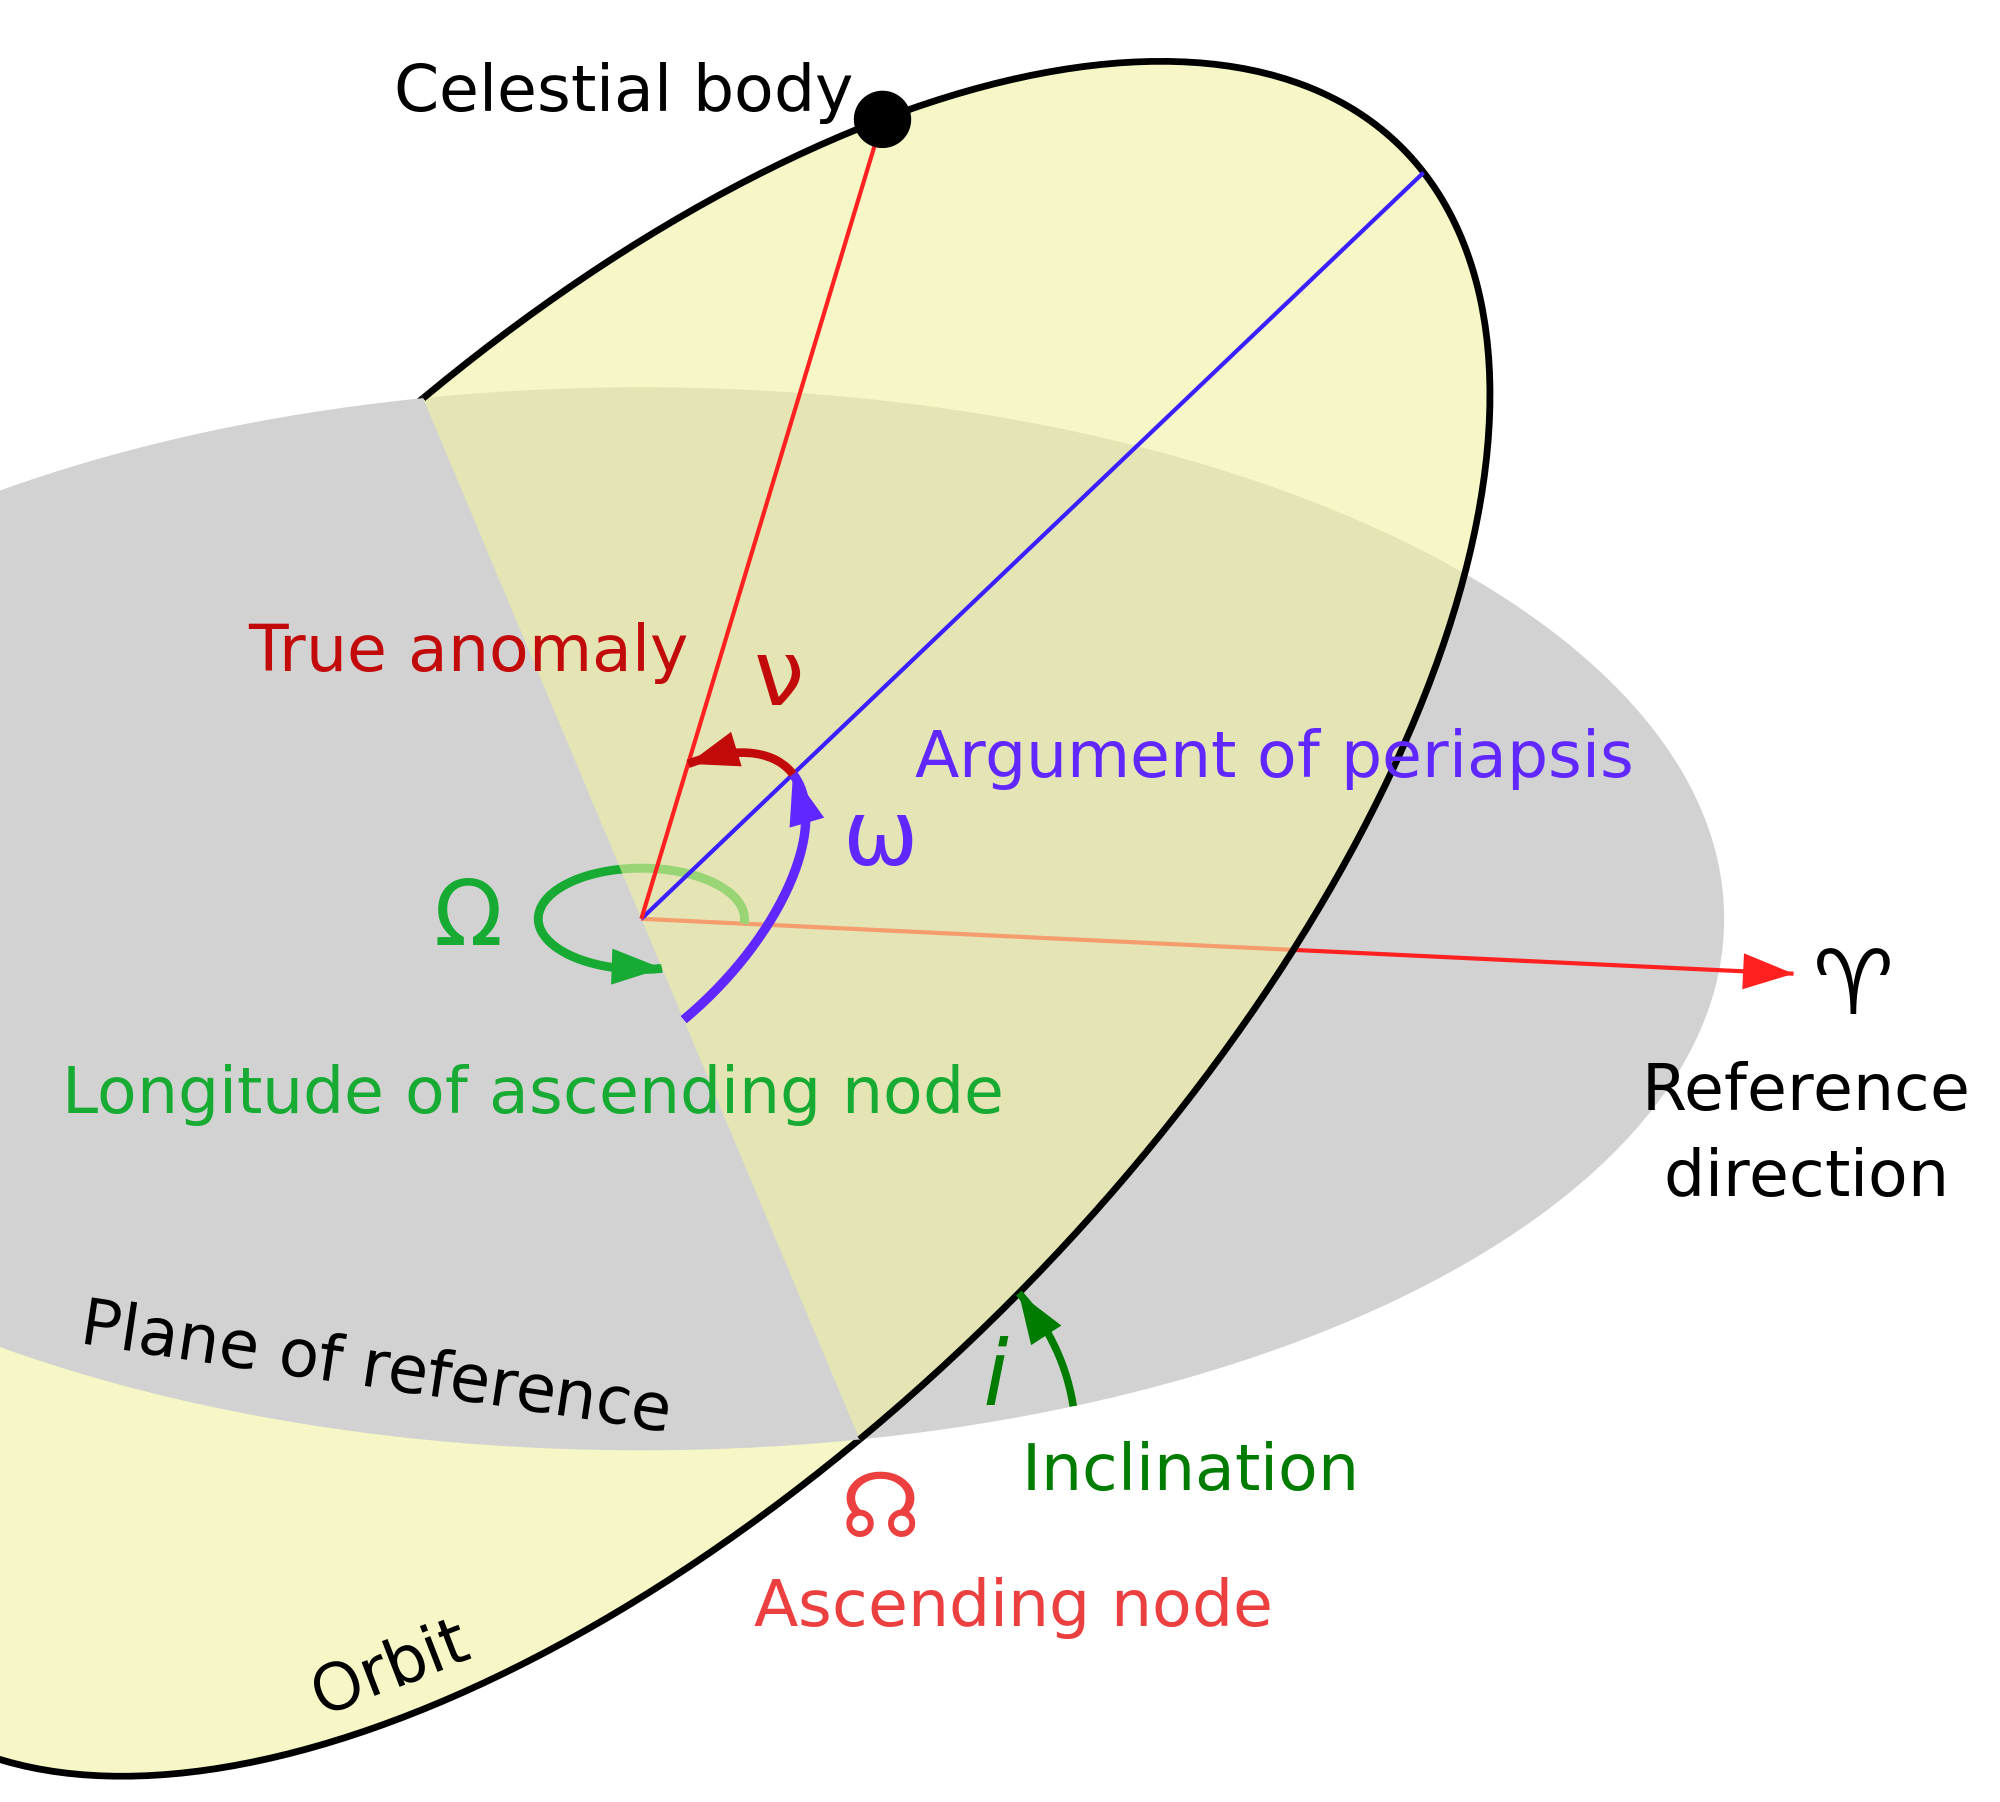
\includegraphics[width=.8\textwidth]{doc/thesis/0_figures/Orbit_elements.png}
        \caption{}
        \label{fig:kepler_elements}
    \end{subfigure}
    \begin{subfigure}[b]{0.47\textwidth}
        \centering
        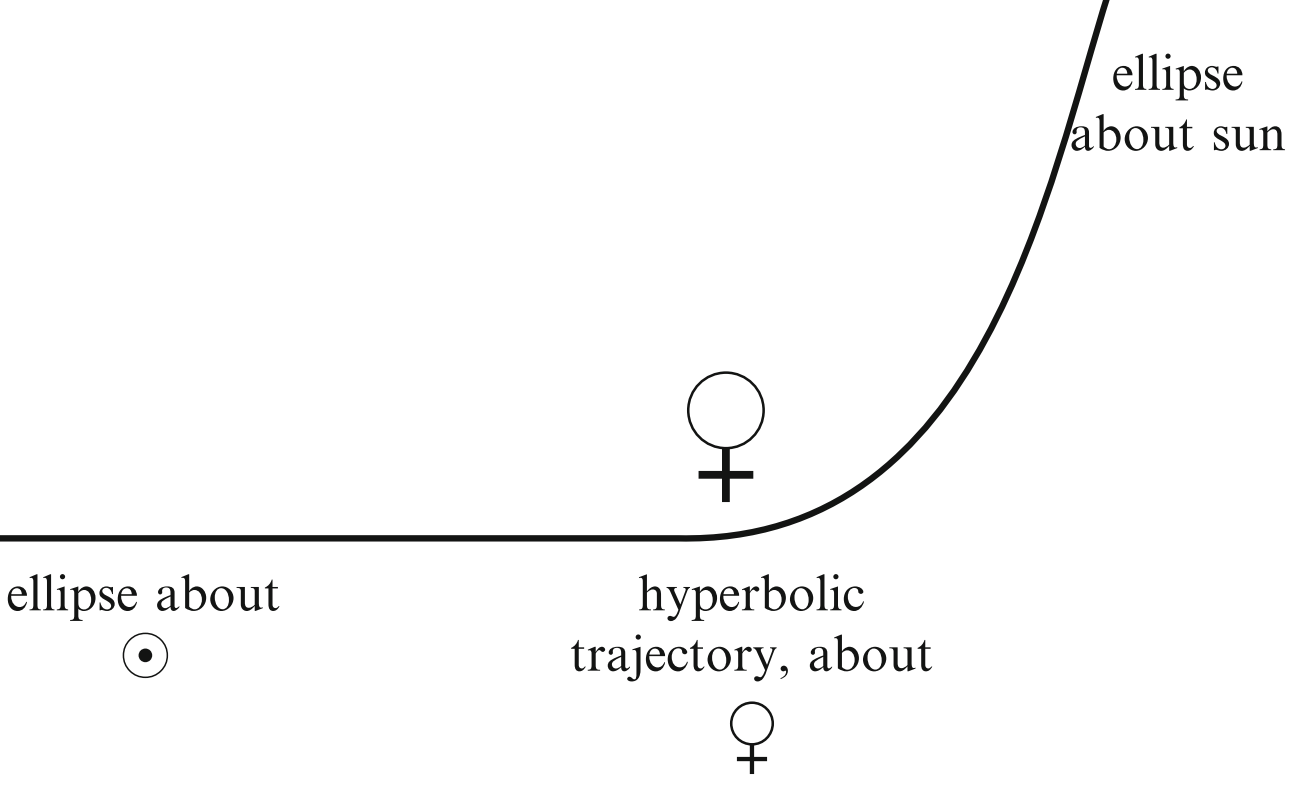
\includegraphics[width=\textwidth]{doc/thesis/0_figures/Hyperbolic_trajectory.png}
        \caption{}
        \label{fig:hyperbolic_orbit}
    \end{subfigure}
    \label{fig:astrodynamics}
    \caption{Important astrodynamic definitions and relations. (a) Modified Keplerian elements \cite{Commons2019Orbit}. (b) A closed orbit around the Sun (\gls{sun}) becomes a hyperbolic trajectory about another body, in this example Venus (\gls{venus})~\cite{Hintz2015FundamentalsAstrodynamics}.}
\end{figure}

Fly-by scenarios in the Solar System are often closed orbits around the Sun, i.e. \gls{e}$_{\astrosun} < 1$ while they are hyperbolic trajectories in the reference frame of the target, i.e. \gls{e}$_{\venus} > 1$. An example is given in Figure~\ref{fig:hyperbolic_orbit}. A high relative velocity and the small gravitational force exerted by a \gls{sssb} result in a trajectory closer to a straight line than the bend trajectory presented in Figure~\ref{fig:hyperbolic_orbit}. 

Most asteroids move on orbits with low eccentricity while comets often have high eccentricities~\cite{ChamberlinCometDistribution}. The eccentricity distribution is caused by the origin of asteroids and comets. While asteroids mostly origin from the main belt which is a nearly circular region, comets enter the inner Solar System from far out, i.e. comets' aphelion is far from the Sun resulting in high eccentricities.

\subsection{Image Rendering}
Rendering is the process of creating \gls{2d} images from \gls{3d} objects. A virtual \gls{3d} world with objects is created which is used to calculate \gls{2d} images. Light sources and cameras produce artificial illumination and define which part of the world is being captured. A rendering engine calculates the pixel values to generate the final image based on energy conservation by using the rendering equation~\cite{Kajiya1986TheEquation}.

\subsubsection{Path Tracing}
Path tracing is a special form of ray tracing. Ray tracing is a rendering technique where the path of light rays is traced to generate pixels while simulating effects of encounters with objects. Path tracing does not branch into an exponentially growing number of rays when being reflected or refracted but only a single path is followed. Path tracing cuts computation time dramatically compared to ray tracing in scenes with a lot of reflection, refraction and shadow rays per pixel~\cite{Kajiya1986TheEquation}. Path tracing can simulate different effects, such as reflection, refraction, scattering and dispersion. There are four types of rays: camera rays, reflection rays, transmission rays and shadow rays. Reflection and transmissions can be further categorised as either diffuse, glossy or singular. Path tracing is a popular rendering technique where a high degree of realism is necessary since it is a realistic simulation of light transport. However, the high degree of realism created by path tracing requires substantial computational power~\cite{Vasiou2018ACost}.

\subsubsection{3D Models and Shaders}
A \gls{3d} model is a set of vertices in \gls{3d} space linked by surfaces. The most common type of \gls{3d} models are polygonal meshes. Polygonal meshes are shell models that consist of polygons. A vertex is a corner of a polygon, i.e. every triangle has three vertices and every tetrahedron has four vertices. A face refers to the surfaces that make up a \gls{3d} model. Depending on the rendering environment, \gls{3d} models can have varying levels of detail and their surface can have different properties such as reflection, refraction and transmission~\cite{FoundationCyclesIntroduction}.

A shader is used to calculate effects of interactions of a ray and objects during the rendering process. Shaders provide a flexible method to influence the rendering outcome during the rendering process. Shaders can be used to change the positions of vertices, colours, lighting and surface properties by using equations. Complex surface structures and texture can be generated procedurally with shaders. Shaders are commonly executed on \glspl{gpu} since \gls{gpu} hardware is well suited for this task~\cite{Pharr2010ChapterMaterials, Sans2017ACUDA, Spath2018AdvancedThMAD}.

Shaders that influence the surface of an object use a \gls{bsdf}. \glspl{bsdf} are a mathematical function that describes light scattering behaviour of a surface of a \gls{3d} model. Several shader classes such as diffuse, glossy, refraction and transparent shaders create the respective effect based on \glspl{bsdf}~\cite{FoundationCyclesIntroduction, Pharr2010ChapterMaterials}.

\subsubsection{Field of View}
The \gls{fov} defines the visible extent of a camera view in \gls{3d} scene. Vectors that point to the edges of the \gls{fov} can be constructed from geometric considerations resulting in
\begin{align}
    e_{i} = v_d \pm \frac{v_j \times s_k}{2 \times f}, \label{eq:fov_edge}
\end{align}
where $e_{i}$ is a vector for the $i^{th}$ edge of the \gls{fov}, $v_d$ is the direction vector of the camera, $v_j$ is the vector pointing right or up in the \gls{fov} plane, $s_k$ is the camera sensor width or height and $f$ is the focal length. The left and right edge vectors, $e_{left}$ and $e_{right}$, are calculated with the vector $v_r$ pointing right in the \gls{fov} plane and the sensor width $s_w$. The upper and lower edge vectors, $e_{upper}$ and $e_{lower}$  are calculated with the vector $v_r$ pointing up in the \gls{fov} plane and the sensor height $s_h$.

In addition to the extent of the \gls{fov} within the image plane, rendering requires the \gls{fov} to be clipped to a minimum and maximum distance. Clipping defines which objects appear in a rendered scene. Clipping is necessary to limit the required computational power for rendering. 

\subsubsection{Photometric calibration} \label{sec:photo_cal}
Photometric calibration is the process of correcting raw images from a sensor to a common level of brightness. Differences can originate from varying exposure times, gains or different camera sensors~\cite{Bergmann2018OnlineSLAM}. Photometric calibration uses a photometric systems, such as the \gls{ubv}, which are reference systems with which star magnitude measurements can be compared for a given band of the system~\cite{Bessell1979UBVRIPhotometry}.

The apparent magnitude of a star is converted into photon flux density \gls{flux_d} relative to magnitude 0 by using,
\begin{align}
    F = 10^{-0.4 \times m}, \label{eq:mag_flux}
\end{align}
where \gls{m} is the apparent star magnitude. Given the apparent magnitude of a specific band, the photon flux density \gls{flux_d} of a reference object can be calculated using
\begin{align}
    F = F_0 \times \frac{\Delta\lambda}{\lambda} \times 10^{-0.4 \times m}, \label{eq:comp_flux_0mag}
\end{align}
where \gls{flux_0} is the photon flux density at magnitude 0, \gls{dlambda} is the wavelength bandwidth, \gls{lambda} is the centre wavelength and \gls{m} is the object's magnitude. The required constants to calculate the photon flux of an object from its magnitude in a given band are presented in Table~\ref{tab:ubv_constants}.

\begin{table}[htb]
    \centering
    \caption{Constants for calculating photon fluxes using the \gls{ubv}~\cite{Bessell1979UBVRIPhotometry}.}
    \label{tab:ubv_constants}
    \begin{tabular}{l|l|l|l}
        \textbf{Band} & \textbf{Centre wavelength \gls{lambda} [\SI{}{\nano\meter}]} & \textbf{$F_0$ [\SI{1e-26}{\watt\per\square\meter\per\hertz}]} & \textbf{$\frac{\Delta\lambda}{\lambda}$}[~] \\ \hline
        U             & 0.36                       & 1810        & 0.15             \\
        B             & 0.44                       & 4260        & 0.22             \\
        V             & 0.55                       & 3640        & 0.16            
    \end{tabular}
\end{table}

Consequently, the reference photon flux for one pixel of the \gls{ccd} \gls{fref} is calculated using
\begin{align}
    F_{ref} = F \times \frac{A \times A_{pixel}}{f^2 \times \pi}, \label{eq:comp_flux_pix}
\end{align}
where \gls{flux_d} is the photon flux density, \gls{a} is the aperture area, \gls{a_pixel} is the area of a pixel and \gls{f} is the focal length of the instrument.

In the last step, the calibration factor~\gls{calibfactor} is calculated. It is defined as
\begin{align}
    f_c = \frac{F_{ref} \times \alpha}{I_{ref}}, \label{eq:comp_cal_fac}
\end{align}
where \gls{fref} is the reference flux, \gls{alpha} is the albedo and \gls{iref} is the reference intensity. Multiplying the image with \gls{calibfactor} produces the calibrated image.

The effect of photometric calibration is delineated in Figure~\ref{fig:t_photometry}. Photometric calibration corrects the brightness difference of a set of images towards a common brightness level~\cite{Bergmann2018OnlineSLAM}.
\begin{figure}[htb]
    \centering
    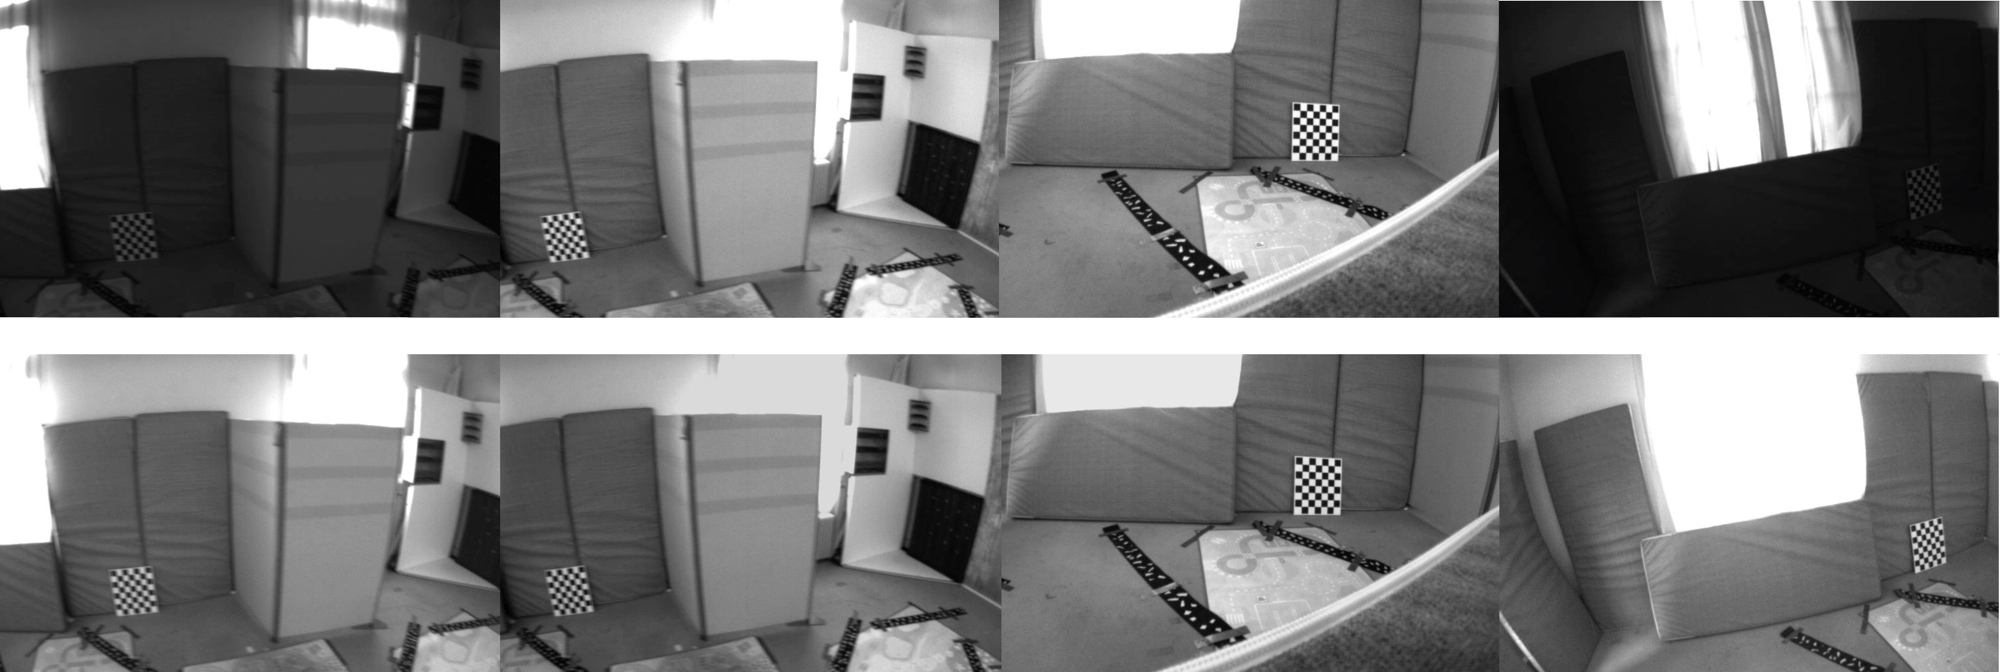
\includegraphics[width=\textwidth]{doc/thesis/0_figures/photo_calib.jpg}
    \caption{Image series before (top) and after (bottom) photometric calibration which eliminated the brightness differences~\cite{Bergmann2018OnlineSLAM}.}
    \label{fig:t_photometry}
\end{figure}

\subsection{Computer Vision} \label{sec:t_cv}
\Gls{cv} is the science of extracting information from digital photos and videos by mimicking the human vision system using a computer. \Gls{cv} encompasses a wide field of activities, from image formation, processing, detecting and matching features, image segmentation and \gls{3d} reconstruction~\cite{szeliski2010computer}. \Gls{cv} is the computer based variant of photogrammetry which is tasked with obtaining information about physical objects and the environment from photographic images~\cite{Kasser2002DigitalPhotogrammetry}. The most common approach for \gls{3d} reconstruction is stereo-photogrammetry, also referred to as computer stereo vision. Stereo-photogrammetry applies the binocular vision principle of the human vision system to obtain structural information from images~\cite{do2019review}. Since most, if not all, deep space missions have a visual imager instrument on-board, \gls{cv} provides a useful framework to obtain the \gls{3d} structure of an observation target. A similar problem is the \gls{sfm} approach where the motion of the camera creates the different perspective.

\subsubsection{Pinhole Camera Model}
All \gls{cv} problems require a model of a camera. The most commonly used model in \gls{cv} is the pinhole camera. Figure~\ref{fig:pinhole_cam} gives a simple overview of the important parts of the pinhole model.

\begin{figure}[htb]
    \centering
    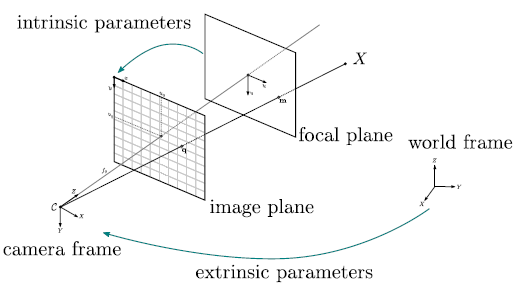
\includegraphics[width=\textwidth]{doc/thesis/0_figures/sfm/pinholeCamera.png}
    \caption{Overview of the components of the pinhole camera model~\cite{openMVG}. The camera intrinsic parameters model the optical distortions, the extrinsic parameters model the camera position and orientation. The image plane is the plane of the \gls{ccd} using u,v coordinates. The focal plane is the plane where the focus of the optical system is.}
    \label{fig:pinhole_cam}
\end{figure} 

The pinhole camera model can be described using the $3\times4$ camera matrix \gls{k} defined as
\begin{align}
    \textbf{K} = \begin{bmatrix}
        f\times k_u & 0           & c_u \\
        0           & f\times k_v & c_v \\
        0           & 0           & 1   \\
    \end{bmatrix} 
    \begin{bmatrix}
        \textbf{R} & t
    \end{bmatrix}, \label{eq:camera_m}
\end{align}
where \gls{f} is the distance between the focal plane and the image plane, \gls{k_u} and \gls{k_v} are scaling factors, \gls{c_u} and \gls{c_v} are the coordinates of the principle point on the image plane, \gls{r} is a $3\times3$ rotation matrix and \gls{t} being a $3\times1$ translation vector. The first matrix of \gls{k} reflects the camera intrinsic parameters while the second matrix describes the extrinsic parameters.
More sophisticated pinhole camera models also include distortions. These can include one or more factors for radial and tangential distortions.

The conversion between object coordinates and pixel coordinates is obtained from geometric considerations of the pinhole camera model shown in Figure~\ref{fig:pinhole_cam} and is defined as
\begin{align}
    u_{pix} = 2 \times \frac{f}{s_w} \times \frac{\hat{v}_r \cdot p}{\hat{v}_d \cdot p + 1} \times \frac{(r_u - 1)}{2}, \label{eq:pix_conversion} 
\end{align}
%x_pix = ss * (f_over_w_ccd_2 * np.dot(right_norm, vec) / np.dot(direction, vec) + 1.) * (res_x - 1) / 2.
where $u_{pix}$ is the u-coordinate of the pixel in the image frame, $f$ is the focal length, $s_w$ is the sensor width, $v_r$ is the unit vector pointing right in the image plane, $p$ is the Cartesian coordinate vector of a star, $v_d$ is the direction vector of the \gls{fov} and $r_u$ is the number of pixels in u-direction. Similarly, the conversion for v-coordinate of a pixel $v_{pix}$ is obtained by replacing the sensor width $s_w$ with the sensor height $s_h$, $v_r$ by the unit vector $v_u$ pointing up in the image plane and the number of pixels in u-direction $r_u$ by the number of pixels in the v-direction $r_v$. The vectors $v_r$ and $v_u$ are calculated by subtracting $v_d$ from the field of view edge vectors $e_{right}$ and $e_{upper}$ as defined in Equation \ref{eq:fov_edge}.

\subsubsection{Structure-from-Motion}
\Gls{sfm} can be considered the inverse process to rendering, i.e. creating \gls{3d} models from \gls{2d} images. \gls{sfm} uses multiple views of the same object from different camera positions to reconstruct its geometry. \Gls{sfm} encompasses the recovery of the \gls{3d} structure of an object as well as camera poses~\cite{szeliski2010computer}. Depth information is obtained through the motion parallax created by the moving camera. Generic steps of an \gls{sfm} processing pipeline are shown in Figure~\ref{fig:sfm_steps}.

\begin{figure}[htb]
    \centering
    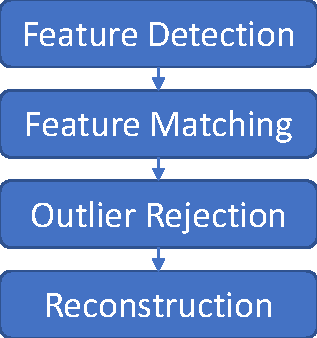
\includegraphics[width=.25\textwidth]{doc/thesis/0_figures/sfm/SfM.pdf}
    \caption{Generic steps of a \gls{sfm} processing pipeline.}
    \label{fig:sfm_steps}
\end{figure}

Figure \ref{fig:sfm_geometry} shows a generic observation geometry. A camera at different positions with feature points on their respective image plane and the relation between this feature point and the object point are depicted. 

\begin{figure}[htb]
    \centering
    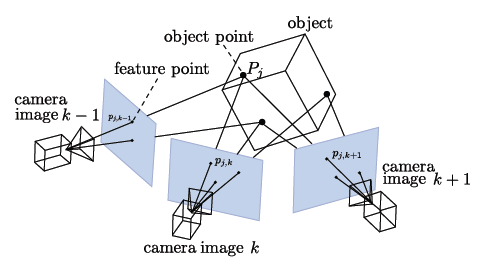
\includegraphics[width=\textwidth]{doc/thesis/0_figures/sfm/sfm_geometry.png}
    \caption{Generic observation geometry in a \gls{sfm} problem~\cite{andrews2019asteroid}. The \gls{3d} structure can be reconstructed from several point observations and intrinsic camera parameters.}
    \label{fig:sfm_geometry}
\end{figure}

To reconstruct \gls{3d} points from an image series, correspondence between images needs to be found. This is achieved by detecting features in an image that can be detected and matched in multiple images. A feature can be described as a local, meaningful and detectable part of an image. Features are being used because of their high information content. Features can be image regions of sudden change, shape features or texture contours. Commonly detected features are corners, edges, junctions, blobs and lines~\cite{Tareen2018ABRISK}. These features are described using feature descriptors which assign a distinct identity to the described feature for later matching. A range of different feature detection algorithms  exist, sometimes with a ready to use algorithm. While most feature detectors are combined with a distinct feature descriptor, it is possible to interchange these. Feature detectors are tasked with detecting feature-points in an image. Feature points are also referred to as key-points or interest-points. A common requirement for good feature descriptors and detectors is that both should be scaling, rotation and affine invariant. The most commonly known feature detectors and descriptor pairs are \gls{sift}, \gls{surf}. \gls{orb}, KAZE and \gls{akaze}~\cite{Tareen2018ABRISK}.
% Add SIFT description?
After features are detected and described in all images, these features need to be matched, i.e. an algorithm identifies the same feature in multiple images. Depending on the descriptor, either an L1 or L2 norm for a scalar descriptor or the hamming distance for binary descriptor are used. Feature matching can be carried out between image pairs or between a longer series of images. Different geometries can be described using different mappings. The homography matrix \gls{H_m} describes mapping of coordinates from two different views and is defined as
\begin{align}
    x'_i = \textbf{H}x_i, \label{eq:homography_m}
\end{align}
where \gls{x_i}$'$ are the coordinates of point $i$ in the second image, \gls{x_i} are the coordinates of point $i$ in the first image and \gls{H_m} is the homography matrix. However, \gls{H_m} describes only a purely rotating or moving camera capturing a planar scene~\cite{schonberger2016structure}.
The fundamental matrix \gls{F_m} describes the relation between two images of the same scene for a moving camera. It relates points of uncalibrated images and is defined as
\begin{align}
    {x'_i}^{T}\textbf{F}x_i = 0, \label{eq:fundamental_m}
\end{align}
where \gls{x_i}$'$ are the coordinates of point $i$ in the second image, \gls{x_i} are the coordinates of point $i$ in the first image and \gls{F_m} is the fundamental matrix. The epipolar line
\begin{align}
    l'_i = \textbf{F}x_i, \label{eq:epipolar_l}
\end{align}
where \gls{l_i} is the epipolar line, \gls{F_m} is the fundamental matrix and \gls{x_i} are the coordinates of a point in the first image. This line constitutes all possible positions of point \gls{x_i}$'$.

If additionally, the camera intrinsics are taken into account, the fundamental matrix becomes the essential matrix \gls{E_m} which is defined as
\begin{align}
    \textbf{E} = \textbf{K}'^{T}\textbf{F}\textbf{K}, \label{eq:essential_m}
\end{align}
with \gls{E_m} being the essential matrix, \gls{k}$'$ being the camera matrix of the second view, \gls{F_m} being the fundamental matrix as defined in Equation~\ref{eq:fundamental_m} and \gls{k} being the camera matrix of the first view. Therefore, the essential matrix is intended for use in conjunction with calibrated images where the camera intrinsic parameters are available.

If sufficient number of points are being mapped correctly using one of the transformations from Equations \ref{eq:homography_m}, \ref{eq:fundamental_m} or \ref{eq:essential_m}, the points are geometrically verified.

However after geometric verification, there might still be outliers. Therefore, outlier rejection is performed as an additional step to remove incorrect matches. Several algorithms such as \gls{ransac}~\cite{Fischler1981RandomCartography}, \gls{acransac}~\cite{moisan2012automatic}, \gls{msac}~\cite{wang2009generalized} and \gls{prosac}~\cite{Chum2005MatchingConsensus} are used for outlier removal. All of these algorithms aim at robustly estimate the correct model and remove outliers. The result of this step is the view graph that relates the different views to each other with images as nodes and pairs as edges~\cite{schonberger2016structure}.

Using the view graph as an input, the reconstruction process produces a \gls{3d} point cloud. A point cloud is a set of independent points with coordinates in \gls{3d} space. There are two principle methods for reconstruction, incremental and global. In case the image set is unordered, the more common approach is to use the incremental approach~\cite{schonberger2016structure}.

Incremental reconstruction starts with an initial pair of views. Selecting this initial pair is a critical step as the reconstruction algorithm might not converge after using a bad initial pair. Typically, starting with a scene with many overlapping camera views constitutes a robust initialisation and results in higher accuracy because of the redundant information from many images~\cite{schonberger2016structure}.
Consequently, additional images are registered to the current model based on corresponding features which can be used to triangulate additional points in already registered images. This step can includes estimating the pose of a camera and also the camera intrinsic parameters for uncalibrated images. Triangulation is an essential step of making \gls{sfm} robust by adding redundant information about existing points in a model and adding additional points to increase the coverage of the model~\cite{schonberger2016structure}. To help these algorithms to converge, it is possible to provide initial pose estimates, so called priors.
Image registration and triangulation are separate process although their results have a strong link. Therefore, errors of one can increase the error in the other, i.e. if the pose estimation during image registration has an error, this error propagates to the position estimate of a triangulated point. To make this process more robust Bundle Adjustment is used. It is the combined refinement of camera pose and point position estimate. A commonly used algorithm is the Levenberg-Marquardt algorithm to minimise the error~\cite{schonberger2016structure, Moulon2013AdaptiveEstimation}.

Global reconstruction uses all images in a common reference frame. While incremental reconstruction accumulates errors through adding views step-by-step, global reconstruction attempts to distribute these residuals equally for all reconstructed points. Therefore, global reconstruction pipelines try to get rid of the problem of accumulating error of incremental \gls{sfm}~\cite{Moulon2013GlobalMotion}.
For using the global method, it is necessary to calculate the essential matrix for all image pairs as the initial step. Commonly, rotation estimation is separated from translation and structure estimation. First a consistent set of rotations are computed in a global frame based on relative rotations of input pairs. Second, camera translations are estimated as well as the structure of the object.

To improve the stability of either \gls{sfm} approach, it is possible to feed priors into the camera intrinsic and extrinsic parameter estimation which are then used as initial guess for the optimisation process.

Both, incremental and global \gls{sfm} methods produce a sparse point cloud as an output. Additionally, they estimate the intrinsic and extrinsic camera parameters. As a next step the sparse point cloud can be densified using \gls{mvs} techniques~\cite{Pagani2011DenseImages}. Image pairs with their camera positions are being used to calculate depth maps. These depth maps are fused and filtered to increase the number of points of the point cloud. This process mimics human depth perception and uses this information to improve the accuracy of its point clouds.

In the next step, the point cloud is converted into a \gls{3d} model by estimating a mesh surface from the point cloud. In addition, outliers are detected and removed from the scene. Different approaches can be used which yield different results. while some techniques only use strongly supported faces, i.e. faces that are supported by many points of the point cloud, other methods also include weakly supported surfaces due to e.g. obstructions~\cite{Jancosek2014ExploitingSurfaces}. The output of these methods are a rough surface model of a 3D object.
A common algorithm for creating a mesh from a point cloud is the Delaunay Tetrahedralisation. For this algorithm, a set of \gls{3d} points $P$ is triangulated to not contain any point of $P$ within the circumscribed sphere of any tetrahedron (3-simplex). The Delaunay tetrahedralisation is often used since it provides a unique solution to the triangulation problem~\cite{vu2012high}.
To increase the accuracy of a rough surface model, the underlying mesh can be further refined. Especially in cases where only a sparse point cloud was used to create the rough mesh, refinement can improve the model accuracy substantially. One such algorithm for mesh refinement is variational multiview stereovision. It is a local optimisation approach, which can be used since the initial mesh captures the main features of the final structure and thus local optimisation is unlikely to be trapped in local minima~\cite{Faugeras1998VariationalProblem, vu2012high}.

The final step in \gls{3d} reconstruction is texturing the surface model. Ideally, the camera poses and the surface model are exact which would make texturing simple. However, in most cases the texturing step requires dealing with inaccuracies in both, the camera poses and the surface model. Other effects such as differing illumination and exposure, unreconstructed occluding objects, varying image scales have to be overcome as well. Texturing is often separated in selecting the images to use for texturing and optimising the resulting image set for consistency~\cite{Waechter2014LetReconstructions}.
Image selection algorithms can be categorised by either blending multiple images per face to achieve consistent texture across patches. Another approach is to use only a single image per face. Both approaches come with advantages and disadvantages~\cite{Waechter2014LetReconstructions}.
Furthermore, colours need to be adjusted, especially because of differences in exposure and illumination. This process attempts to correct seams between patches by photometric adjustments. Colour adjustment can be split into local or global adjustments. Local adjustment tries to smooth the transition between texture patches by introducing gradients in the texture luminances for example by using heat diffusion equations~\cite{Velho2007ProjectivePhotography}. For global adjustment, the luminance correction terms are calculated for a global optimum~\cite{Lempitsky2007SeamlessMaps}.

\subsection{Image Compression and Processing}
Digital image processing is the use of a digital computer to process digital images through algorithms. Relevant to this work are image compression (cf. Section~\ref{sec:t_compress}), Gaussian filtering  (cf. Section~\ref{sec:t_gauss}) and image down-sampling  (cf. Section~\ref{sec:t_downsample}).

\subsubsection{Compression} \label{sec:t_compress}
Data compression is tasked with encoding information using less bits than the original representation. Other terms for data compression are source coding or bit-rate reduction~\cite{Mahdi2012ImplementingTechnique}. Two principle methods of compression exist, lossless and lossy compression. While it is possible to recover all information after lossless compression, lossy compression accepts a certain irreversible loss of information to achieve higher compression ratios.
Lossless compression uses statistical redundancy to decrease the number of bits necessary to encode the same information. This process is completely reversible. There are many lossless compression algorithms such as Huffman coding, arithmetic coding or Lempel-Ziv algorithms~\cite{Bocharova2009CompressionMultimedia}.

Lossy compression is not a reversible process, i.e. some of the information is lost and cannot be recovered. The idea of lossy compression is that different image properties are perceived with varying degrees of precision and are therefore not equally important. Lossy compression is a trade-off between compression ratio and data distortion. Audio data can be encoded with a lossy scheme by decreasing the accuracy of acoustic components that are beyond the capabilities of most humans. Another example is, that the human eye is more sensitive to changes in brightness (luminance) than it is to changes in colour (chrominance). Therefore, compression can lose colour information without having a strong influence of the perceived image quality. As a result, images for compression often use a luminance-chrominance representation. The components in such a representation are almost uncorrelated and it is easier to reduce colour information while keeping luminance information. Commonly known formats for lossy compression are MP3 or JPEG. Most lossy compression algorithms are based on transform coding, especially \gls{dct}~\cite{Bocharova2009CompressionMultimedia}.

Image compression is a sub-discipline of data compression. A common format for lossless compression is \gls{png} which relies on a Lempel-Ziv algorithm and Huffman-coding. Two types of image compression techniques commonly used for lossy compression are the \gls{dct} and \gls{dwt}. \Gls{dct} is used for example in the \gls{jpeg} format and \gls{dwt} is used for example in the \gls{jp2} format.

The Lempel-Ziv algorithm used in \gls{png} replaces repeating sections of data with a single copy and references to that copy. Huffman coding is a form of entropy coding which estimates the number of occurrences of symbols and encodes symbols with higher probability using the least amount of bits.

\Gls{dct} is a type of Fourier transform, hence it expresses finite data as a sum of cosines. In contrast to the Fourier transform itself, it employs however only real components. \Gls{dct} compresses data in form of discrete data blocks. Images can be compressed with differently sized image parts such as $8\times8$ pixels, commonly used in JPEG~\cite{Bocharova2009CompressionMultimedia}.
The frequency response of the \gls{dct} improves with longer harmonic functions. Hence, \gls{dct} does not have favourable compression characteristics if an image has many small details or contours~\cite{Bocharova2009CompressionMultimedia}.

\Gls{dwt} uses a wavelet transform, hence it expresses data using a set of wavelet base functions. \gls{dwt} has an advantage over \gls{dct} for finite, non-periodic or non-stationary signals. As a result, \gls{dwt}-based compression is particularly well suited to compress images with high frequency components, such as a star background~\cite{Bocharova2009CompressionMultimedia}. Through the properties of wavelets, their use in a \gls{dwt} results in a hierarchical structure of the output data. Therefore, when transforming an image with a \gls{dwt}, the lowest lowpass subband of an image contains a rough approximation of a given image. Consequently, every additional higher frequency subband adds additional detail to the image. Additionally, only small parts of an image contain high frequency components, such as contours and sharp details, therefore these subbands can be strongly compressed using lossless algorithms since these subbands mostly contain zeros~\cite{Bocharova2009CompressionMultimedia}. The hierarchical structure of an image transformed with \gls{dwt} is depicted in Figure~\ref{fig:jp2_hierarchy}.
\begin{figure}[htb]
    \centering
        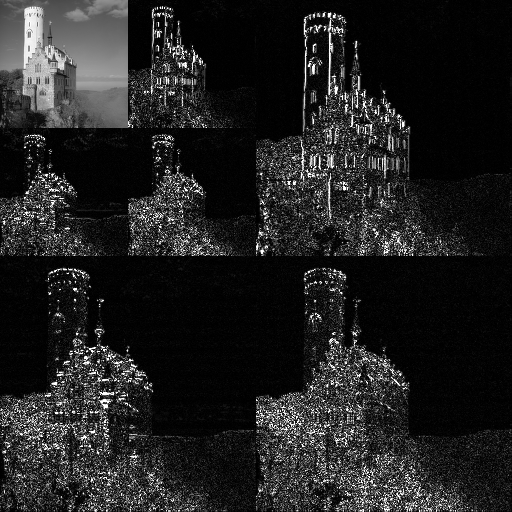
\includegraphics[width=.7\textwidth]{doc/thesis/0_figures/jp2_jpeg/Jpeg2000_2-level_wavelet_transform-lichtenstein.png}
        \caption{Hierarchical structure of an image transformed with 2-level \gls{dwt} \cite{Commons20192-levelTransform-lichtenstein}.}
        \label{fig:jp2_hierarchy}
\end{figure}

A comparison of an image compressed with \gls{jpeg} and with \gls{jp2} with roughly similar compression ratio is shown in Figure~\ref{fig:jpg_jp2_comparison}. It is clearly visible that artefacts are created around the contours in the \gls{jpeg} image in contrast to the \gls{jp2} image, despite the higher compression ratio of the \gls{jp2} image.
\begin{figure}[htb]
    \centering
    \begin{subfigure}[b]{0.7\textwidth}
        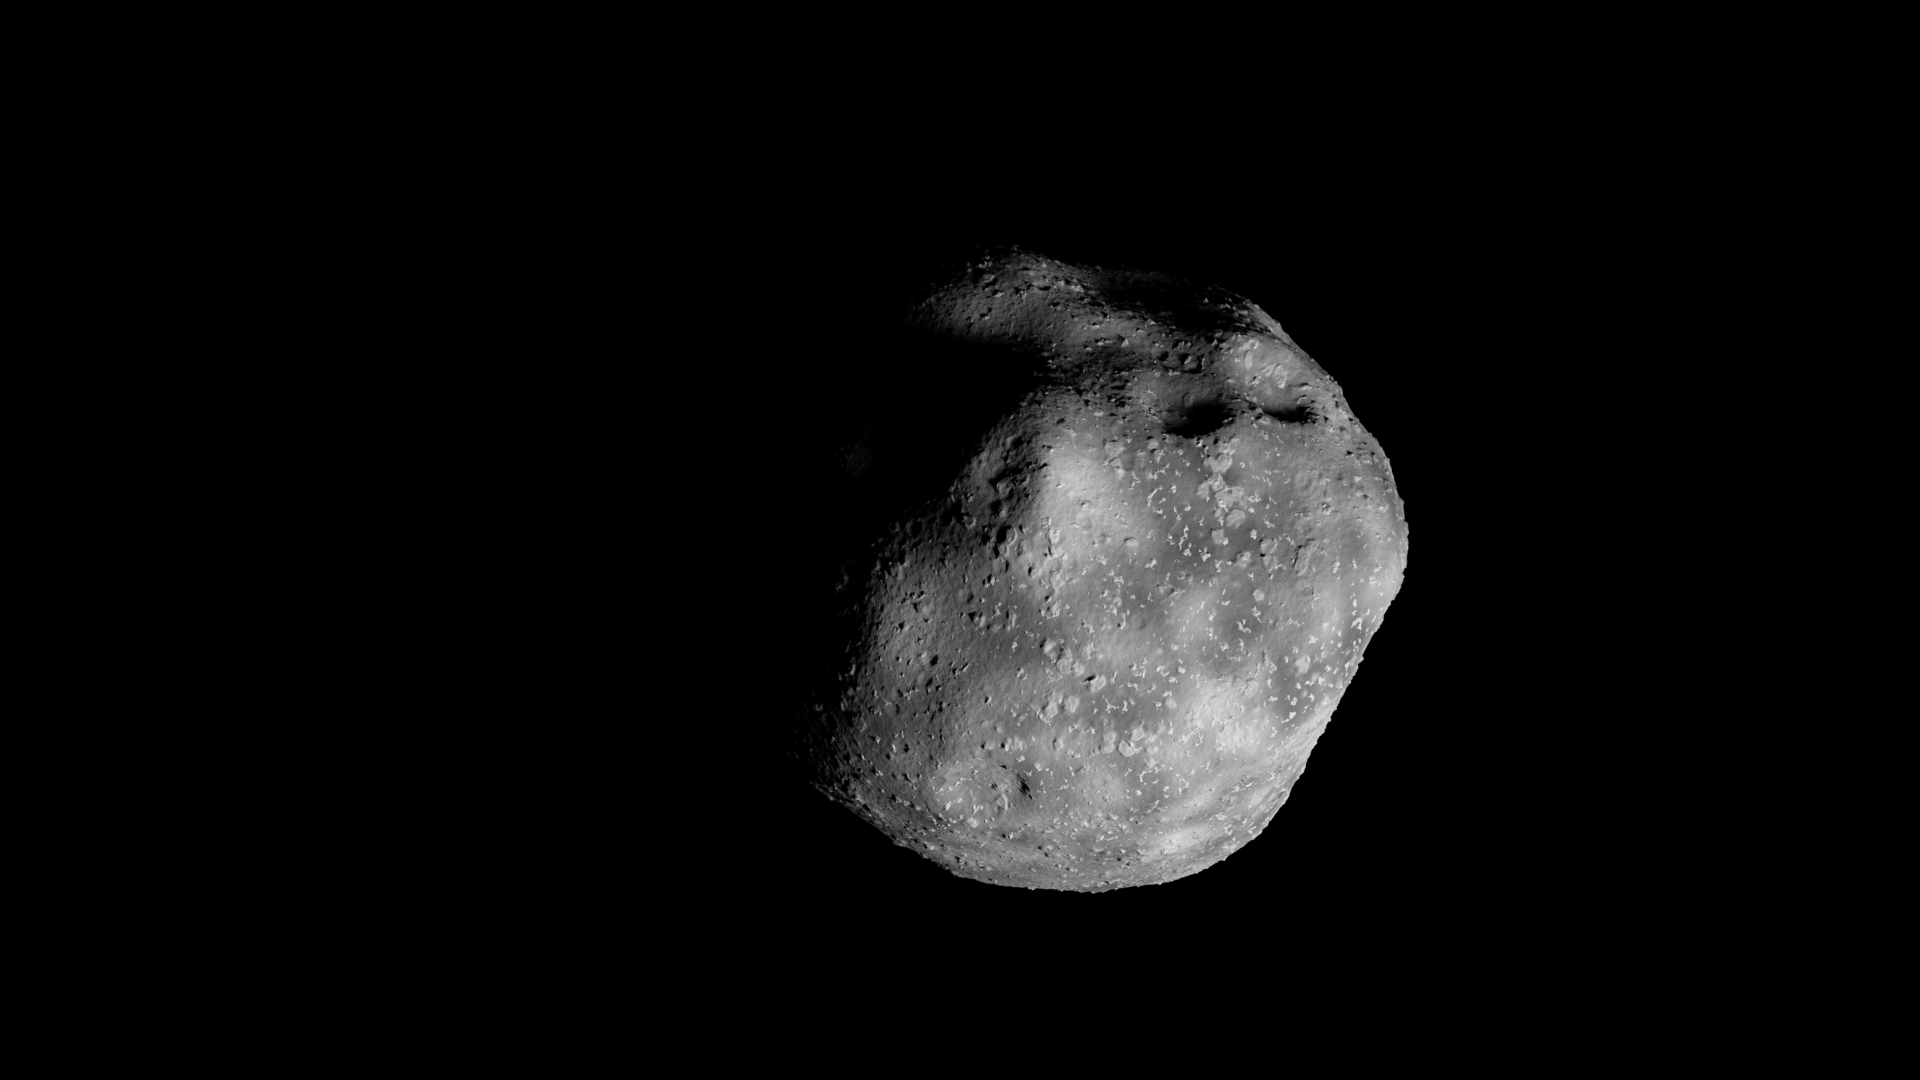
\includegraphics[width=\textwidth]{doc/thesis/0_figures/jp2_jpeg/orig.png}
        \caption{Original image without compression.}
        \label{fig:jpg_jp2_oirg}
    \end{subfigure}
    \\
    \begin{subfigure}[b]{0.48\textwidth}
        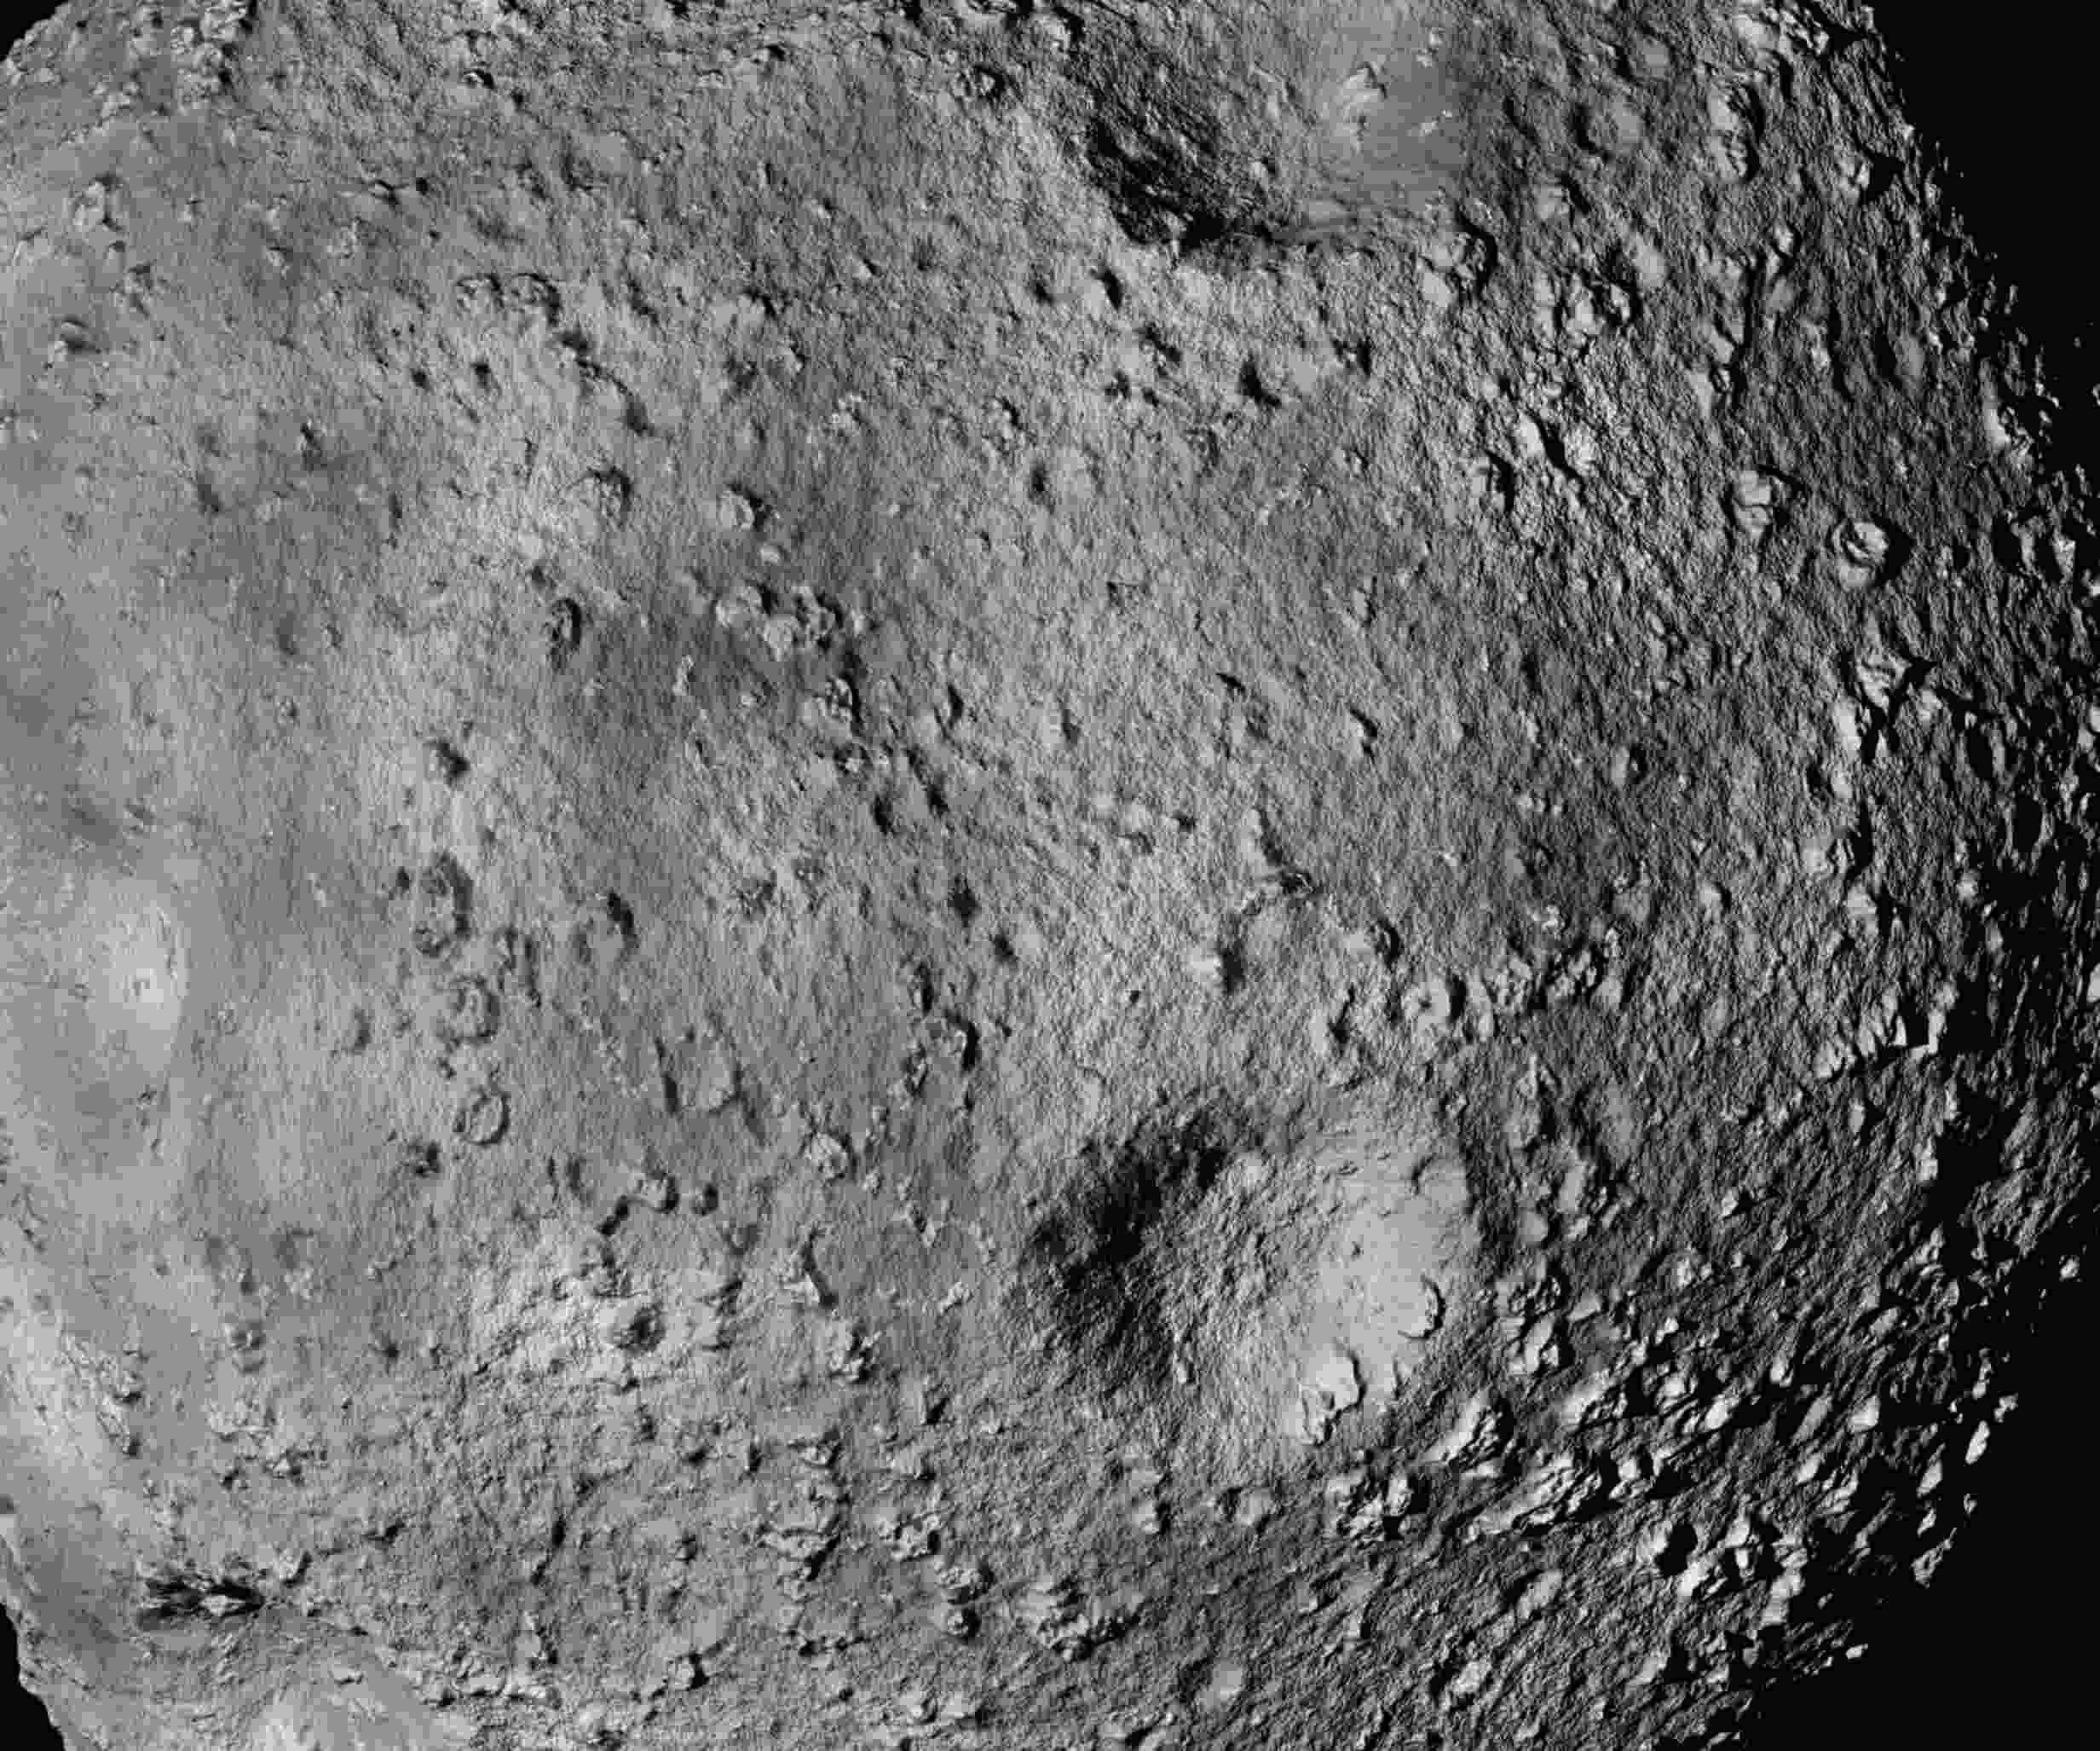
\includegraphics[width=\textwidth]{doc/thesis/0_figures/jp2_jpeg/proc_5.jpg}
        \caption{}
        \label{fig:jpg_jp2_jpeg}
    \end{subfigure}
    \begin{subfigure}[b]{0.48\textwidth}
        \includegraphics[width=\textwidth]{doc/thesis/0_figures/jp2_jpeg/proc_11.png}
        \caption{}
        \label{fig:jpg_jp2_jp2}
    \end{subfigure}
    \caption{Comparison of compression images compressed with different algorithms. Despite having a higher compression ratio, the \gls{jp2} image produces a better result for a \gls{sssb} image. (a) Raw image without compression. (b) Image compressed with \gls{dct} using the \gls{jpeg} format with a compression ratio of 61.2:1. (c) Image compressed with \gls{dwt} using the \gls{jp2} format with a compression ratio of 64.3:1.}
    \label{fig:jpg_jp2_comparison}
\end{figure}

\subsubsection{Gaussian Filtering} \label{sec:t_gauss}
Gaussian Filtering refers to convolving an image with the \gls{2d} Gaussian function. It is used to blur images and remove noise. The \gls{2d} Gaussian function \gls{G}$(x,y)$ with a mean of zero is defined as
\begin{align}
    G(x,y) = \frac{1}{2\pi \sigma^{2}}e^{-\frac{x^2+y^2}{2\sigma^2}}, \label{eq:gauss_2d}
\end{align}
where \gls{sigma} is the standard deviation of the Gaussian distribution, and $x$ and $y$ are the coordinates.
In its theoretical version, the Gaussian distribution would extend to infinity. To be practically applied in a digital system, the Gaussian distribution needs to be cut at a certain distance from the centre. The range over which the filter is applied is the kernel size which is normally related to its standard deviation, since \SI{99}{\percent} of the distribution falls within 3 standard deviations. In addition, the Gaussian distribution needs to be discretised to be usable in a digital system. The \gls{2d} Gaussian filter is rotationally symmetric and larger standard deviation result in more blurring due to a wider peak.

\subsubsection{Down-sampling with Local Means} \label{sec:t_downsample}
Down-sampling is the process of reducing the number of pixels in an image. When down-sampled with local means, it refers to taking the average of a small set of pixels and using it as the new value of a single pixel. For example, if an image shall be reduced by a factor of two, the value of four pixels of the input are averaged for a single pixel of the output. In the example below a $4\times4$ matrix is down-sampled by a scaling factor of two to give a $2\times2$ matrix.
\begin{align*}
    \begin{bmatrix}
        1  & 2  & 3  & 4\\
        5  & 6  & 7  & 8\\
        9  & 10 & 11 & 12\\
        13 & 14 & 15 & 16\\
    \end{bmatrix} 
    \rightarrow 
    \begin{bmatrix}
        3.5  & 5.5\\
        11.5 & 13.5\\ 
    \end{bmatrix}
\end{align*}



\clearpage
\section{\Acrlong{sispo}} \label{sec:sispo}

\gls{sispo} is a software package developed in python. It is separated in different sub-packages. The two main sub-packages are the \textit{sim} and the \textit{reconstruction} package. The third sub-package provides several image compression algorithms to test effects on reconstruction.

The software package is hosted on GitHub using a git version control system. Furthermore, the GitHub project management tools are used, including automated KanBan based projects, issue tracking and pull requests.

The most important python dependencies of \gls{sispo} are:
\begin{itemize}
    \item astropy: Astronomy package developed by \cite{robitaille2013astropy} and \cite{price2018astropy}
    \item Blender: 3D creation suite
    \item \textit{NumPy}: Scientific computing for python
    \item opencv: Computer vision library used for image processing
    \item OpenEXR: \gls{hdr} image reading and writing
    \item Orekit: Space dynamics library
\end{itemize}

It was attempted to reduce dependencies to other libraries as much as possible. Originally, both \textit{scikit-image} and \textit{opencv} were used. After a small benchmark between the two libraries, it was evident that \textit{opencv} performs three to seven times faster compared to \textit{scikit-image} (cf. \ref{sec:cvskimage}. Hence \textit{scikit-image} was completely replaced with equivalent \textit{opencv} functions. Additionally, it was attempted to use the \textit{opencv} package to replace the \textit{OpenEXR} dependency since it is not easy to install. However, this is currently not possible as the \textit{OpenEXR} implementation of \textit{opencv} does not provide an alpha channel and is generally less flexible.

To ease development, numerous parameters are silently assigned default values if not provided e.g. for an instrument. Therefore, all parameters should be explicitly set before running a simulation.

\gls{sispo} was developed in an attempt to logically separate the distinct steps involved of the entire processing pipeline. Such modularity eases further development as well as reduce unnecessary library imports to reduce memory consumption.

\subsection{User Interface}
The sispo package can be installed using pip and the GitHub project. If done, it will be installed into the site-packages folder of the used python environment. Additionally, an executable is installed, providing a \gls{cli} as user interface. The most recent possible input arguments are documented in the repository or by using the --help input. The most important arguments for the \gls{cli} are seen in Table \ref{tab:cli_args}.

\begin{table}[htpb]
\caption{Input arguments for sispo \gls{cli}}
\begin{tabular}{p{0.13\textwidth}|p{0.15\textwidth}|p{0.15\textwidth}|p{0.3\textwidth}}
\hline
\textbf{Name}                            & \textbf{Variable Name} & \textbf{Default Value}     & \textbf{Description}                                                                                                      \\ \hline
\multicolumn{1}{l|}{--help}              &                        & ---                        & Prints list of arguments with hints                                                                                       \\
\multicolumn{1}{l|}{-i}                  & i                      & data/input/definition.json & Path to a definition file that defines the settings                                                                 \\
\multicolumn{1}{l|}{-v}                  & v                      & False                      & Verbose output, logging information will also be displayed on STDOUT                                                      \\
\multicolumn{1}{l|}{--cli}               & cli                    & False                      & If the \gls{cli} flag is set, an interactive \gls{cli} will be started. NOT IMPLEMENTED. \\
\multicolumn{1}{l|}{--profile}           & profile                & False                      & If the profile flag is set, Python's cProfile will be used to profile \gls{sispo} execution              \\
\multicolumn{1}{l|}{--no-sim}            & with\_sim              & True                       & If flag is set, simulation step will be skipped                                                                           \\
\multicolumn{1}{l|}{--no-render}         & with\_render           & True                       & If flag is set, rendering step will be skipped                                                                            \\
\multicolumn{1}{l|}{--no-compression}    & with\_compression      & True                       & If flag is set, compression step will be skipped                                                                          \\
\multicolumn{1}{l|}{--no-reconstruction} & with\_reconstruction   & True                       & If flag is set, reconstruction step will be skipped                                                                       \\
\multicolumn{1}{l|}{--sim-only}          & sim\_only              & False                      & If flag is set, only simulation step will be done                                                                         \\
\multicolumn{1}{l|}{--sim-render-only}   & sim\_render\_only      & False                      & If flag is set, only simulation and rendering will be done                                                                \\
\multicolumn{1}{l|}{--render-only}       & render\_only           & False                      & If flag is set, only rendering will be done                                                                               \\
\multicolumn{1}{l|}{--compress-only}     & compress\_only         & False                      & If flag is set, only compression will be done                                                                             \\
\multicolumn{1}{l|}{--reconstruct-only}  & reconstruct\_only      & False                      & If flag is set, only reconstruction will be done                                                                         

\end{tabular}
\label{tab:cli_args}
\end{table}

The standard interface to be used is a \textit{definition.json} file which provides all input parameters in the \gls{json} format.

\gls{sispo} can be imported as a Python module. Execution is then started either by sispo.run() or sispo.main(), which are equivalent.

\subsection{Simulation Module}
The simulation module creates photo-realistic images by simulating a realistic trajectory of a \gls{sssb} and a spacecraft using Orekit. This trajectory and attitude data is then used to render four images per frame, one containing only the \gls{sssb}, one where the view is kept at a constant distance from the \gls{sssb}, one calibration reference image and one that renders a realistic star background using the \gls{ucac4}. Additionally, the date, the spacecraft position, \gls{sssb} position and their distance is stored as metadata. These images are composed to one image using photometry to calibrate the absolute light intensity of the different images in terms of realistic photon fluxes using the Johnson magnitude system \cite{bessel1979ubvri}. The composition process is explained in more detail in section \ref{sec:composition}

A run of the simulation package includes the following steps
\begin{enumerate}
    \item Propagate \label{enum:propagate}
    \item Render
\end{enumerate}

In the propagate step \ref{enum:propagate}, Orekit is used to determine state information of the \gls{sssb} and the spacecraft. The state information includes the date, position and the rotation angles of the \gls{sssb}. Propagation is defined by start and end date, number of steps, the timesampler mode and a slowmotion factor.
The timesampler mode determines whether the steps are distributed linear in time (mode 1, default) or whether an exponential model (mode 2) is used which takes more samples around the encounter. How many samples more are taken can be controlled with the slowmotion factor. Mode 2 is especially helpful when simulating a long period since far from the \gls{sssb} nucleus, there are only minor visible changes over longer periods.

The \textit{sim} sub-package was developed to contain all general information about the environment in the Environment class in order to have one consistent instance for constants. 

All images during the rendering and calibration process use the OpenEXR format to minimise the loss of information in intermediate steps.

The Orekit library runs a \gls{vm} to execute its Java code. Additionally, physical data is required which is currently distributed with the \textit{sim} sub-package. The \gls{vm} and physical data are initialised in the \textit{sim} main module and only afterwards other modules are imported which is why other modules do not include the Orekit initialisation. This approach was taken in order to reduce resource consumption by having several instances of the \gls{vm} running. Propagation is based on Orekit's KeplerianOrbit and KeplerianPropagator classes.

The initial state of the spacecraft is calculated based on the input parameters presented in \ref{tab:sc_enc_paras}. Only the three first parameters need to be given as input in the definition file.

\begin{table}[htb]
    \caption{Parameters that define the encounter state of the spacecraft.}
    \label{tab:sc_enc_paras}
    \begin{tabular}{p{0.23\textwidth}|p{0.06\textwidth}|p{0.62\textwidth}}
        Parameter           & Type  & Description                                                                                                                                                  \\ \hline
        encounter\_distance & float & Minimum distance between SSSB and spacecraft in meters                                                                                                       \\
        with\_terminator    & bool  & Determines whether the terminator is visible at the closest approach                                                                                         \\
        with\_sunnyside     & bool  & Determines whether the spacecraft passes the SSSB on the Sun facing side or the SSSB's side facing away from the Sun                                         \\
        sssb\_state         & tuple & \gls{sssb} state vector, including 3 position and 3 velocity components, at encounter. The spacecraft encounter state is calculated relative to this state vector. The \gls{sssb} state does not need to be set in the  definition file but is calculated based on the \gls{sssb} trajectory and encounter date.
    \end{tabular}
\end{table}

\subsubsection{Blender}
To render the \gls{sssb} and calibration images, Blender is used. A set of predefined settings is used for each scene while some parameters can be changed via the definition file. The rendering engine \textit{Cycles} is used to render photo-realistic, physics-based images from the Blender scenes.

Blender is interfaced using its Python bindings which need to be compiled manually (cf. \ref{sec:setup}. To control the behaviour of Blender the BlenderController class is used. It handles setting all defaults such as a black background and the creation of the default scene, SssbOnly. In addition, the BlenderController interfaces to the star catalogue and the compositor.

Since the images are composed and calibrated at a later step, described in \ref{sec:composition}, the settings shown in Table \ref{tab:color_space} are selected to not change the rendered raw images with Blender while saving.

\begin{table}[htpb]
\caption{Blender settings relevant to color space and are fixed to get raw images out of the Blender rendering process.}
\label{tab:color_space}
\begin{tabular}{p{0.25\textwidth}|p{0.08\textwidth}|p{0.57\textwidth}}
\textbf{Name}        & \textbf{Value} & \textbf{Description}                                                                                         \\ \hline
Color mode           & RGBA           & Use RGB and alpha channel.                                                                                   \\
Sequencer colorspace & Raw            & Color space sequencer uses linear color space.                                                               \\
View transform       & Raw            & No color space conversion.                                                                                   \\
Look                 & None           & No artistic effect is applied before color space conversion.                                                 \\
Film transparent     & True           & World background is transparent, i.e. alpha values can be used for image composition and proper occultation.
\end{tabular}
\end{table}

\begin{table}[htpb]
\caption{Blender settings that can be changed.}
\label{tab:blender_settings_input}
\begin{tabular}{p{0.12\textwidth}|p{0.1\textwidth}|p{0.7\textwidth}}
\textbf{Name}       & \textbf{Default Value} & \textbf{Description}                                                                                                         \\ \hline
Device     & AUTO          & Device used for rendering. "AUTO" attempts to use GPU, if not available uses CPU. \\
Samples    & 6             &                                                                                                                     \\
Exposure   & 0             & Exposure in stops, applied before display transform.                                                                \\
Resolution & ---           & Array determining number of pixels in x- and y-direction.                                                          
\end{tabular}
\end{table}

\subsubsection{Star Rendering} \label{sec:stars}
The background stars are rendered based on the star catalogue \gls{ucac4}. This catalogue includes stars up to magnitude 16. The \gls{fov} is determined based on the spacecraft camera in the SssbOnly scene. The edges of the \gls{fov} are calculated using the following equations

\begin{align}
    e_{right} = v_d + v_r \times \frac{s_w}{2 \times f}, \label{eq:edge_right} \\
    e_{left} = v_d - v_r \times \frac{s_w}{2 \times f}, \label{eq:edge_left} \\
    e_{upper} = v_d + v_u \times \frac{s_h}{2 \times f}, \label{eq:edge_upper} \\
    e_{lower} = v_d - v_u \times \frac{s_h}{2 \times f}, \label{eq:edge_lower}
\end{align}
where $e_{i}$ is a vector for the i-th edge of the \gls{fov}, $v_d$ is the direction vector of the camera, $v_r$ is the vector pointing right, $s_w$ is the camera sensor width, $s_h$ is the camera sensor height and $f$ is the focal length. These vectors are converted into their respective right ascension and declination using

\begin{align}
    \delta = \arcsin{(z)}, \label{eq:declination} \\
    \alpha = \arccos{\left(\frac{x}{\cos{\delta}}\right)} + \pi, \label{eq:right_ascension}
\end{align}
where $\delta$ is the declination and $\alpha$ the right ascension. The \gls{fov} is then defined as the right ascension and declination of the center point as well as the width and height. Using this information the star catalogue returns a list of visible stars with their right ascension and declination as well as their magnitude.

The star background is created by generating an image with twice the size of final image. The coordinates are converted from the right ascension and declination of each star into pixel coordinates. Afterwards setting the pixel value of each colour channel to the flux calculated from the magnitude. The resulting image is Gaussian filtered and downscaled to the final image size using local means. The alpha values of the entire image are set to one. Star background images are stored in the OpenEXR format. An example image is presented in Fig. \ref{fig:star_rendering}.

\begin{figure}[htpb]
    \centering
    
\includegraphics[width=\textwidth]{doc/thesis/0_figures/star_rendering/Stars_2017-08-15T115856-171000.png}
    \caption{Star background rendered using the method described in Section \ref{sec:stars}.}
    \label{fig:star_rendering}
\end{figure}


\subsubsection{Composition} \label{sec:composition}
Rendered images of Blender vary in absolute light intensity thus requiring calibration. For calibration, the Blender output is normalised by comparing the theoretical and real intensity of a calibration disk in the same conditions. This calibration is based on the Johnson magnitude system, also called the UBV photometric system \cite{bessel1979ubvri}. The V-band is used which is centered around \SI{550}{\nano\meter}.

The starting point for composition is a set of four images with the prefixes SssbOnly (cf. Fig. \ref{fig:comp_sssbonly}), SssbConstDist (cf. Fig. \ref{fig:comp_sssbconstdist}), LightRef (cf. Fig. \ref{fig:comp_lightref}) and Stars (cf. Fig. \ref{fig:comp_stars}). SssbOnly represents the view from the instrument. SssbConstDist is a follower camera at a constant distance of \SI{1000}{\kilo\meter} from the \gls{sssb}. LightRef is a defined reference model. Stars is an image of the star background. These images are then composed to a single final image. An example image set is shown in Fig. \ref{fig:comp_imageset}.

\begin{figure}[htb]
    \centering
    \begin{subfigure}[b]{0.47\textwidth}
        \centering
        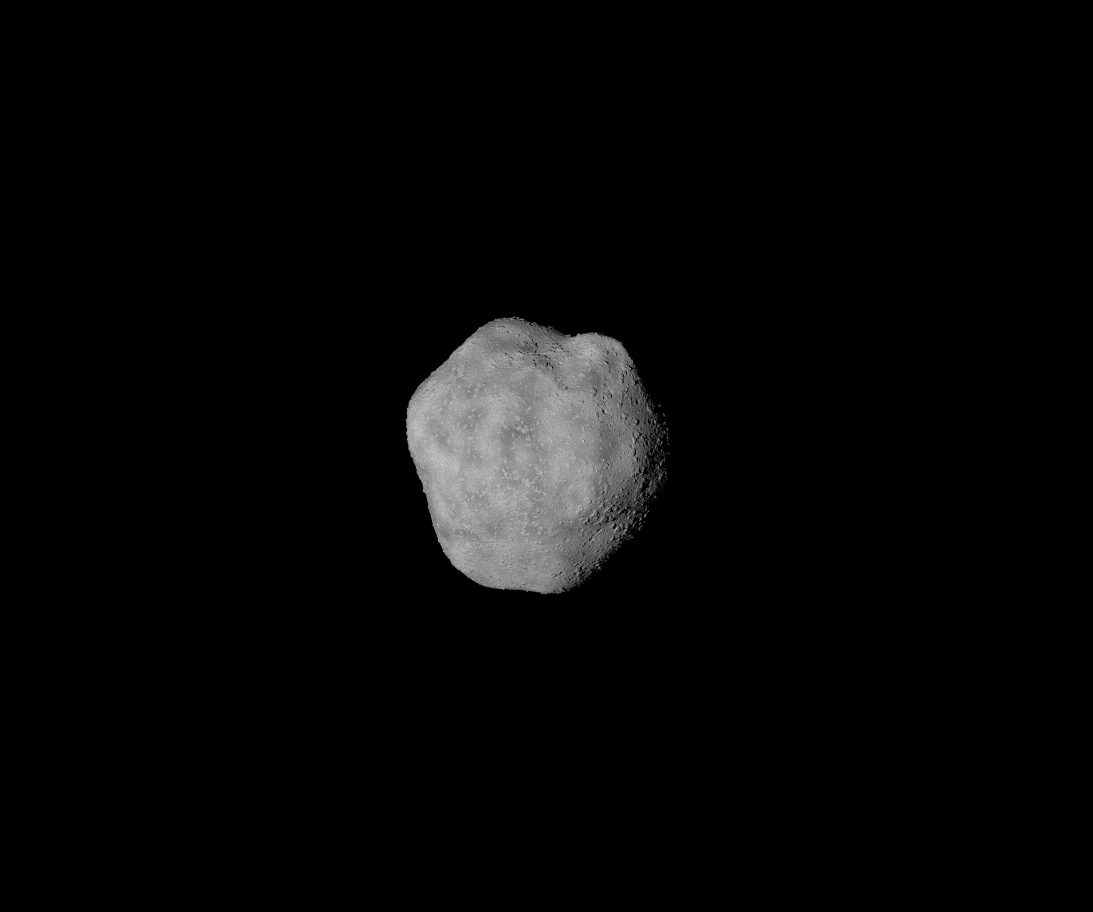
\includegraphics[width=\textwidth]{doc/thesis/0_figures/composition/SssbOnly_2017-08-15T115855-684000.png}
        \caption{SssbOnly}
        \label{fig:comp_sssbonly}
    \end{subfigure}
    \begin{subfigure}[b]{0.47\textwidth}
        \centering
        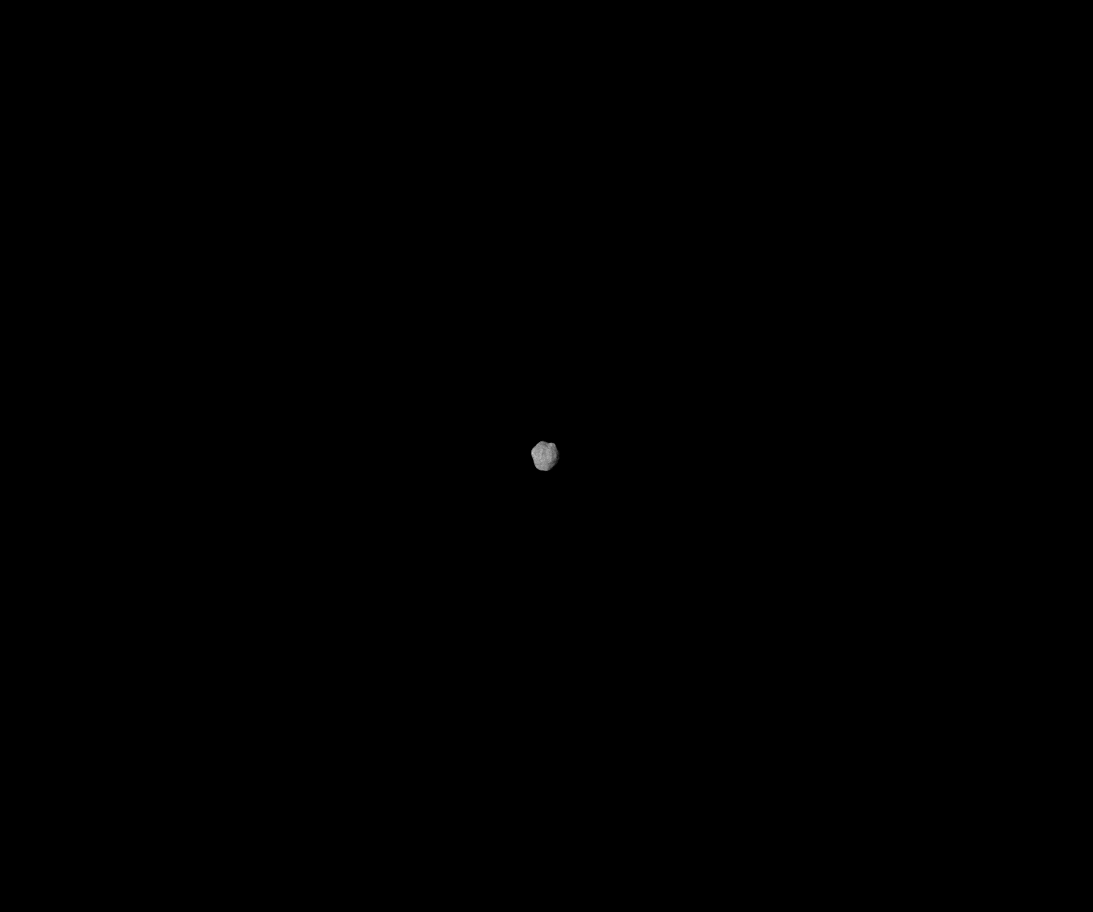
\includegraphics[width=\textwidth]{doc/thesis/0_figures/composition/SssbConstDist_2017-08-15T115855-684000.png}
        \caption{SssbConstDist}
        \label{fig:comp_sssbconstdist}
    \end{subfigure}
    \\
    \begin{subfigure}[b]{0.47\textwidth}
        \centering
        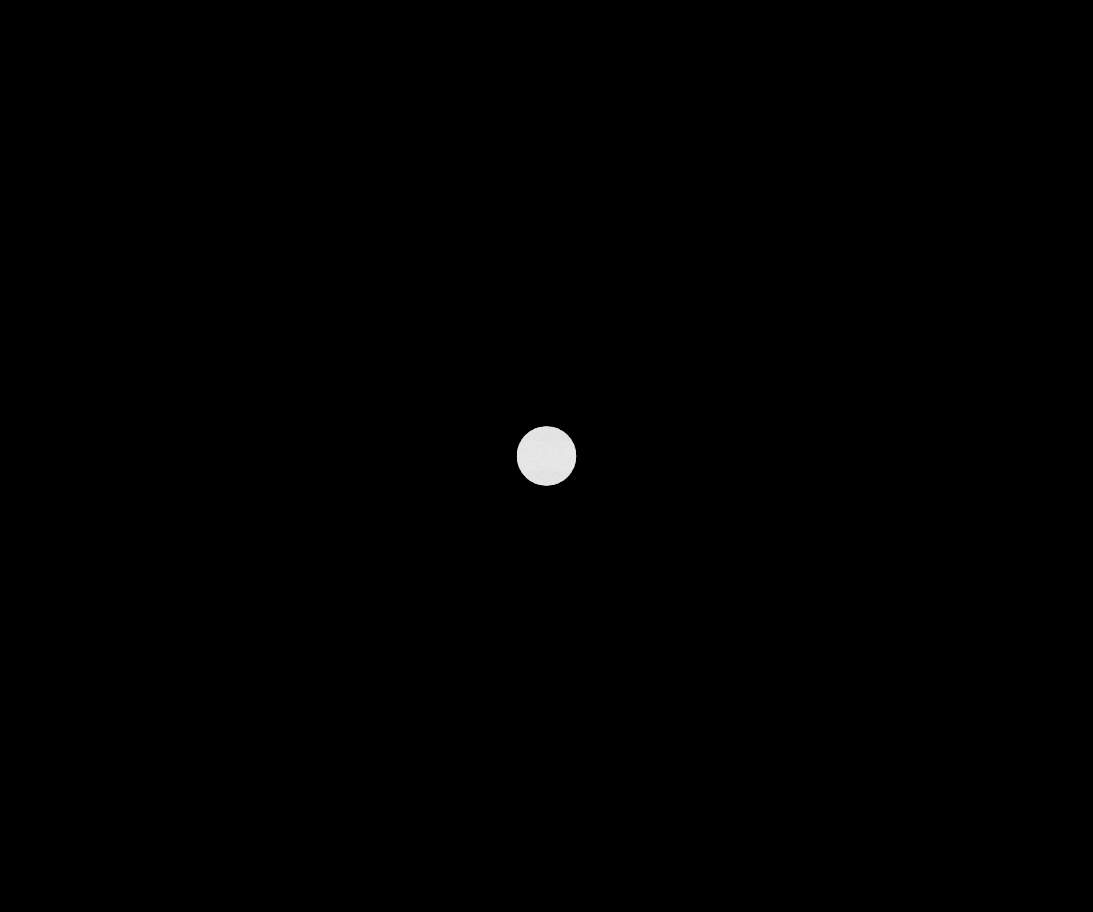
\includegraphics[width=\textwidth]{doc/thesis/0_figures/composition/LightRef_2017-08-15T115855-684000.png}
        \caption{LightRef}
        \label{fig:comp_lightref}
    \end{subfigure}
    \begin{subfigure}[b]{0.47\textwidth}
        \centering
        
\includegraphics[width=\textwidth]{doc/thesis/0_figures/composition/Stars_2017-08-15T115855-684000.png}
        \caption{Stars}
        \label{fig:comp_stars}
    \end{subfigure}
    \caption{Example set of images used for composition to the final rendering output.}
    \label{fig:comp_imageset}
\end{figure}

The reference used for photometric calibration is the solar photon flux in the V-band at \SI{1}{\astronomicalunit} calculated based on \cite{wirth}.

The photon flux is defined as,
\begin{align}
    F = F_0 \times \frac{d\lambda}{\lambda} \times 10^{-0.4 \times m}, \label{eq:comp_flux_0mag}
\end{align}
with $F_0$ being the flux at magnitude 0, $\frac{d\lambda}{\lambda}$ is a factor of 0.16 for the V-band, and $m$ is the object's magnitude. The V-band photon flux at $0~mag$ in SI units is \SI{5.4964e10}{\per\second \per\square\meter}. With a magnitude of $m_{\bigodot} = -26.74~mag$ at a distance of \SI{1}{\astronomicalunit}, the solar photon flux becomes \SI{4.36715206e+20}{\per\second\per\square\meter}.

In the first step, the reference photon flux per pixel is calculated using,
\begin{align}
        F_{ref} = F \times \left(\frac{\SI{1}{\astronomicalunit}}{d_{\bigodot}}\right)^2 \times \frac{A \times pix_A}{f^2 \times \pi}, \label{eq:comp_ref_flux}
\end{align}
where $F$ is the solar flux at \SI{1}{\astronomicalunit}, $d_{\bigodot}$ is the spacecraft distance from the Sun, $A$ is the aperture area, $pix_A$ is the area of a pixel and $f$ is the focal length.

For the star background, every pixel is calibrated according to Eq. \ref{eq:comp_cal_starmap}.
\begin{align}
        pix = pix_0 \times F_0 \times A \times \frac{F_{stars}}{S_{stars}}, \label{eq:comp_cal_starmap}
\end{align}
with $pix_0$ being the original pixel value, $F_0$ being the flux at magnitude 0, $A$ being the aperture area, $F_{stars}$ being the total flux of visible stars and $S_{stars}$ being the summed pixel value of one channel of a starmap.

Depending on the visible size of the \gls{sssb} in the image, either a point source \gls{sssb} image is generated and used or the \gls{sssb} image is calibrated. The point source is necessary if the \gls{sssb}'s nucleus is smaller than a pixel outputting wrong intensities.

The point source image is created by Gaussian filtering a single white pixel at the center of an image, oversized by a factor of five, and then downscaled to the original size using local means.

If the \gls{sssb} image is used, the reference intensity of the image is calculated as the mean of a \SI{70}{} square pixels of the light reference image.

Using the calibration factor defined as
\begin{align}
    f_c = \frac{F_{ref} \times I_{ref}}{\alpha}, \label{eq:comp_cal_fac}
\end{align}
where $F_{ref}$ is the reference flux, $I_{ref}$ is the reference intensity and $\alpha$ is the geometric albedo. Every pixel of the image is multiplied with this factor to produce the calibrated \gls{sssb} image. The star background and the calibrated \gls{sssb} image are merged taking the alpha channels into account. Using the alpha channel information provides proper occultation of the star background by the nucleus. For this, the \textit{film\_transparent} option of the Cycles rendering engine is activated.

The composed image is then multiplied by the quantum efficiency of the \gls{ccd}. This quantum efficiency currently includes all efficiencies to convert incoming photon flux into an electrical signal (pixel value). Afterwards, the image is Gaussian filtered and noise based on a Poisson distribution is added. The standard deviation for Gaussian filtering is calculated to approximate the diffraction pattern, defined as
\begin{align}
    \sigma = 0.45 \times \lambda \times \frac{f}{D}\times \frac{1}{pix_l} \times m, \label{eq:comp_sigma}
\end{align}
where $\sigma$ is the standard deviation, $\lambda$ is the instrument wavelength, $f$ is the focal length, $D$ is the aperture diameter, $pix_l$ is the length of one side of a pixel and $m$ is a multiplier for none diffraction limited systems (in our case $m = 2$. The noisy image is scaled to an interval $[0,1]$ by dividing through the maximum value. In case a point source \gls{sssb} is used, the maximum value is clipped to five times the maximum of the the reference if the maximum value of the merged image is above this threshold. The composed image using the data set shown in Fig. \ref{fig:comp_imageset} is presented Fig. \ref{fig:comp_composed}.

\begin{figure}
    \centering
    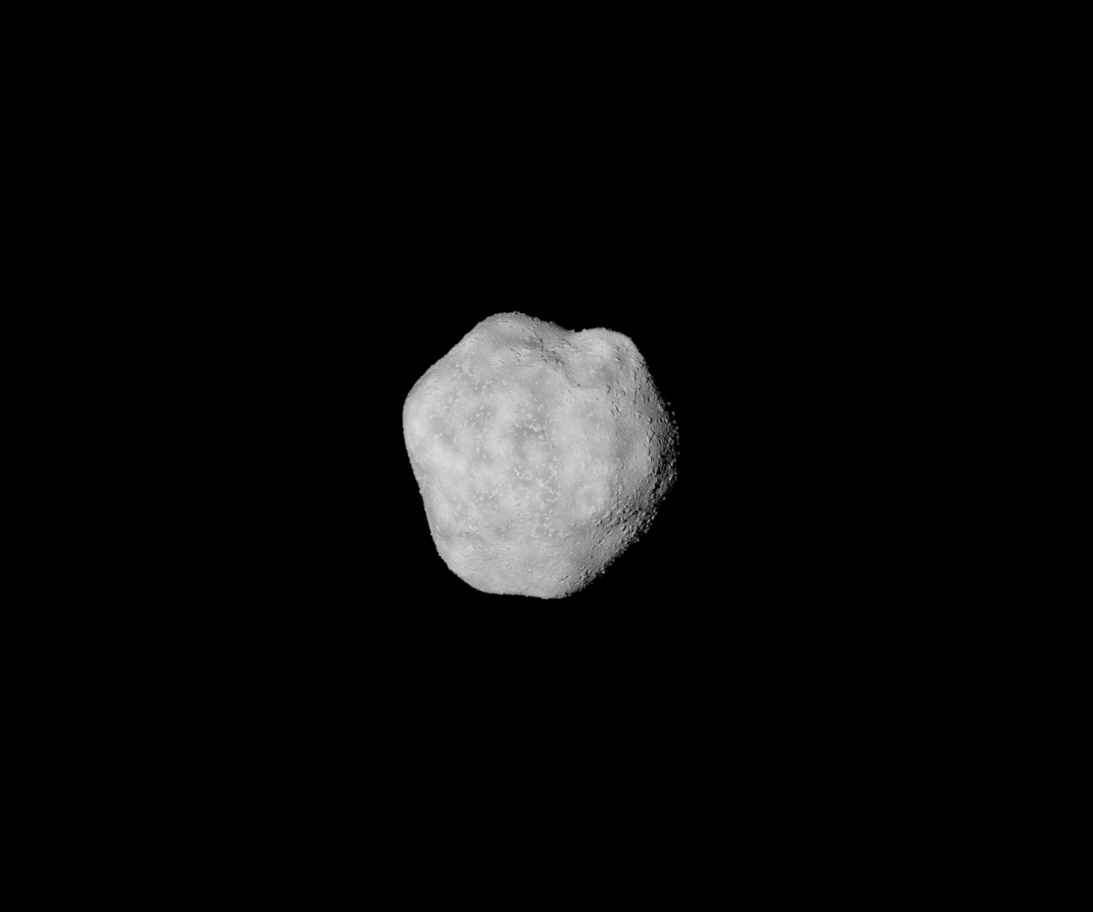
\includegraphics[width=\textwidth]{doc/thesis/0_figures/composition/Comp_2017-08-15T115854-575000.png}
    \caption{Composed image of the four images shown in Fig. \ref{fig:comp_imageset}}
    \label{fig:comp_composed}
\end{figure}

In a final step, the image values are scaled to the bit depth of the \gls{ccd}. The current maximum permissible bit depth is \SI{16}{bit} due to a substantial increase in code complexity for higher bit depths. This feature can be turned off by setting the \textit{with\_clipping} parameter to false.

An additional feature is to add an information box in the lower right corner of the image including the distance to the \gls{sssb} and the date. This feature can be turned off by setting the \textit{with\_infobox} parameter to false.

\subsection{Compression Module}
The compression module provides compression and decompression algorithms. These can be tested against different mission scenarios and image series to investigate the impact of compression and decompression on the scientific quality of the images. Table \ref{tab:compression_format} shows the available compression and decompression algorithms.

\begin{table}[htpb]
\caption{Lossless and lossy compression algorithms provided within \gls{sispo}.}
\label{tab:compression_format}
\begin{tabular}{l|l}
\textbf{Lossless Format} & \textbf{Lossy Formats} \\ \hline
png               & jpeg           \\
exr               & jpeg200        \\
bz2               & tiff           \\
gzip              &                \\
lzma              &                \\
zlib              &               
\end{tabular}
\end{table}

Independent of the algorithm, files are handled equally to. The images are loaded into \textit{NumPy} arrays inside Python to have a common raw format. Before encoding, the information is reduced to \SI{8}{\bit} since the reconstruction module only reads images with \SI{8}{\bit} colour depth correctly. Images are encoded with the respective algorithm and converted into a binary stream. A copy of this data is saved as a file in the raw folder. The raw binary data is then converted back to a \textit{NumPy} array and decoded to retrieve as much information as possible. Finally, the compressed and decompressed data is stored as a png file to not lose any further information.

The formats png, jpeg, jpeg2000 and tiff are implemented using \textit{OpenCV}. There are various settings for each format. A description can be found at \url{https://docs.opencv.org/4.1.2/d4/da8/group__imgcodecs.html#ga292d81be8d76901bff7988d18d2b42ac}.

The most important input parameter that is relevant to all algorithms is the "level" argument which describes either the compression level (from 1 to 9 for bz2, gzip, lzma, zlib and png, higher meaning more compression) or the quality level (from 1 to 10 for jpeg and jpeg2000, higher meaning better quality and less compression).

\subsection{Reconstruction Module}
The reconstruction module can be used to generate a 3D model of an object using a series of images. It provides a full Multi-View Stereo reconstruction data process pipeline. To achieve this, two libraries are used and combined and called using python. The first library is \gls{omvg} by \cite{openMVG}. The second library is \gls{omvs}. 
The common steps for the complete pipeline is comprised of the following steps:
\begin{enumerate}
    \item Read in images [ImageListing in \gls{omvg}]
    \item Compute visual features [ComputeFeatures in \gls{omvg}]
    \item Match computed features between different images [MatchFeatures in \gls{omvg}]
    \item Generate point cloud from matched features [IncrementalSfM in \gls{omvg}]
    \item Export to \gls{omvs} format [openMVG2openMVS in \gls{omvg}]
    \item Increase number of points in point cloud [DensifyPointCloud in \gls{omvs}]
    \item Create a mesh from the point cloud [ReconstructMesh in \gls{omvs}]
    \item Refine the generated mesh [RefineMesh in \gls{omvs}]
    \item Apply texture to mesh to create final 3D model [TextureMesh in \gls{omvs}]
\end{enumerate}

\subsection{Setup} \label{sec:setup}
\gls{sispo} can be setup with Linux and Windows. The default case used in this description is a Windows setup. Known differences or problems under Linux will be pointed out. While it should be possible to use a plain Python environment and pip, a miniconda environment manager was used for development. Also a C compiler is necessary. Linux provides the GCC, for Windows it is easiest to install Microsoft Visual Studio with \gls{msvc} and \gls{msbuild}. Another possibility when using Windows is to use vcpkg\footnote{Found at \url{https://github.com/microsoft/vcpkg}}. However, previously the openMVG and openMVS ports in vcpkg did not work. Vcpkg can also be used with Linux. However, there were unsolvable problems when using vcpkg so everything was installed natively.
For \gls{omvg}, \gls{omvs} and star\_cats it is necessary to have the executables in the correct folder for \gls{sispo} to function.\newline

\begin{figure}
    \dirtree{%
        .1 sispo.
            .2 build.
            .2 data.
                .3 input.
                .3 models.
                .3 sensor\_database.
                .3 UCAC4.
                    .4 u4b.
                    .4 u4i.
            .2 doc.
            .2 sispo.
                .3 compression.
                .3 reconstruction.
                .3 sim.
            .2 software.
                .3 blender.
                .3 miniconda.
                .3 openMVG.
                    .4 build\_openMVG.
                        .5 install.
                    .4 openMVG.
                .3 openMVS.
                    .4 build\_openMVS.
                        .5 install.
                    .4 openMVS.
                .3 star\_cats.
                    .4 build\_star\_cats.
                    .4 star\_cats.
                .3 vcpkg.
    }
    \caption{Directory structure after setup. No files are shown.}
    \label{fig:dir_tree}
\end{figure}
Figure \ref{fig:dir_tree} shows the assumed overall folder structure after installation. No sub-folders of the build folder or any files are shown.

To make \gls{sispo} perform well, it is beneficial to install the Nvidia CUDA Toolkit (https://developer.nvidia.com/cuda-downloads) in case an Nvidia graphics card is available.

In the following enumeration, commands intended to be run in a shell are highlighted with a grey box.

\begin{enumerate}
    \item Clone the GitHub repository onto the local machine \\ \shellcmd{git clone https://github.com/YgabrielsY/sispo.git}. The project provides a software folder which is intended to be used to install all following software.
    \item Setup (conda) environment with dependencies (to software/miniconda folder):
    \begin{enumerate}
        \item orekit 9.3.1, the current version 10.0 had issues when attempted to install. Also orekit needs a data package to function, it is distributed with \gls{sispo} in the sim module folder.
        \item astropy
        \item opencv
        \item OpenEXR\footnote{For Windows the pre-compiled package found at \url{https://www.lfd.uci.edu/~gohlke/pythonlibs/\#openexr} needs to be used because the pip or conda version do not work.}
        \item \textit{NumPy}
        \item Python\footnote{During development Python version 3.7 was used.}
    \end{enumerate}{}
    \item (Especially Windows) Install vcpkg to software/vcpkg folder, follow instructions at \url{https://github.com/microsoft/vcpkg}
    \item Install Blender as a python module (bpy)\footnote{During development Blender version 2.8 was used.}
    \begin{enumerate}
        \item Clone Blender git repository to software/blender/blender \\ \shellcmd{git clone git://git.blender.org/blender.git}
        \item Compile target bpy \shellcmd{make bpy}, this works also for Windows through the make.bat file provided with Blender
        \item When available: Activate CUDA in the cmake project and recompile
        \item Install bpy to python environment\footnote{Follow these instructions \url{https://blender.stackexchange.com/questions/117200/how-to-build-blender-as-a-python-module}}
    \end{enumerate}{}
    \item Install OpenMVG, follow instructions at \\ \url{https://github.com/openMVG/openMVG/blob/master/BUILD.md} or look for hints in the OpenMVG install script in the build folder.
    \begin{enumerate}
        \item Install dependencies according to instructions
        \item Clone OpenMVG GitHub repository to software/openMVG/openMVG \shellcmd{git clone --recursive https://github.com/openMVG/openMVG.git}
        \item Build to software/openMVG/build\_openMVG folder
        \item Install to software/openMVG/build\_openMVG/install folder
    \end{enumerate}
    \item Install OpenMVS, follow instructions at \\ \url{https://github.com/cdcseacave/openMVS/wiki/Building} or look at the OpenMVS install script in the build folder for hints.
    \begin{enumerate}
        \item Install dependencies according to instructions
        \item Clone OpenMVS GitHub repository to software/openMVS/openMVS \shellcmd{git clone https://github.com/cdcseacave/openMVS.git}
        \item Build to software/openMVS/build\_openMVS folder
        \item Install to software/openMVS/build\_openMVS/install folder
    \end{enumerate}
    \item Install star\_cats
    \begin{enumerate}
        \item Clone star\_cats GitHub repository to software/star\_cats/star\_cats \\ \shellcmd{git clone https://github.com/Bill-Gray/star\_cats.git}
        \item Build to software/star\_cats/build\_star\_cats \shellcmd{make}
    \end{enumerate}
    \item Download UCAC4 star catalog to data/UCAC4, use either:
    \begin{enumerate}
        \item the build/data/download\_ucac4.sh script
        \item download the folder u4b and u4i directly from \\ \url{http://casdc.china-vo.org/mirror/UCAC/UCAC4/}
    \end{enumerate}
\end{enumerate}{}

\subsection{Performance}
\subsubsection{Image processing benchmark} \label{sec:cvskimage}
The original codebase used the \gls{skimage} and OpenCV libraries. In order to reduce the number of dependencies, the relevant functions of the two libraries were benchmarked. For this comparison, OpenCV functions were used to create the same behaviour as the respective \gls{skimage} function. The benchmark compares the performance of the Gaussian filter and a special case of image resizing using local means. A set of five images is selected and are shown in Appendix \ref{sec:app_cvskimage}. Two star images were selected due to the large variance in the number of visible stars. The selected images represent extreme cases with 1804 (Stars1) and 51338 stars (Stars2).

Two computers are used for the benchmark. A laptop with \SI{8}{\giga\byte} \gls{ram}, an Intel i7-6700HQ with 4 cores at \SI{2.6}{\giga\hertz} and Windows 10. The second is a workstation computer with \SI{16}{\giga\byte} of \gls{ram}, an Intel i7-8700 with 6 cores at \SI{3.2}{\giga\hertz} and Ubuntu 18.04.3 LTS.

To compare the performance between the two libraries the ratio of execution time is used. The ratio is defined as
\begin{align}
    Ratio = \frac{t_{skimage}}{t_{opencv}}, \label{eq:bm_exec_ratio}
\end{align}
where $t_{skimage}$ is the execution time of \gls{skimage} and $t_{opencv}$ is the execution time of OpenCV. Each command is executed and timed for 1000 times. The lowest value is chosen as the result, since higher values are rather influenced by other processes running on the respective machine than the relevant code snippet itself \cite{timeit2020}.

Figure \ref{fig:bm_comparison} shows the execution time ratios with their averages over set of images. A ratio larger than one corresponds to a longer execution time of \gls{skimage}. OpenCV outperforms \gls{skimage} for both tests on both computers. The maximum absolute difference between pixel values of images is \SI{1.486e-6}{} and \SI{7.153e-7}{} for the Gaussian filtered and the resized images respectively. Such differences are irrelevant considering \gls{ccd} sensor color depths of \SI{16}{bit}.

%Maximum error gauss:  1.4864218655930017e-06
%Maximum error resize:  7.152557373046875e-07

\begin{figure}[htb]
    \centering
    \begin{subfigure}[b]{0.47\textwidth}
        \centering
        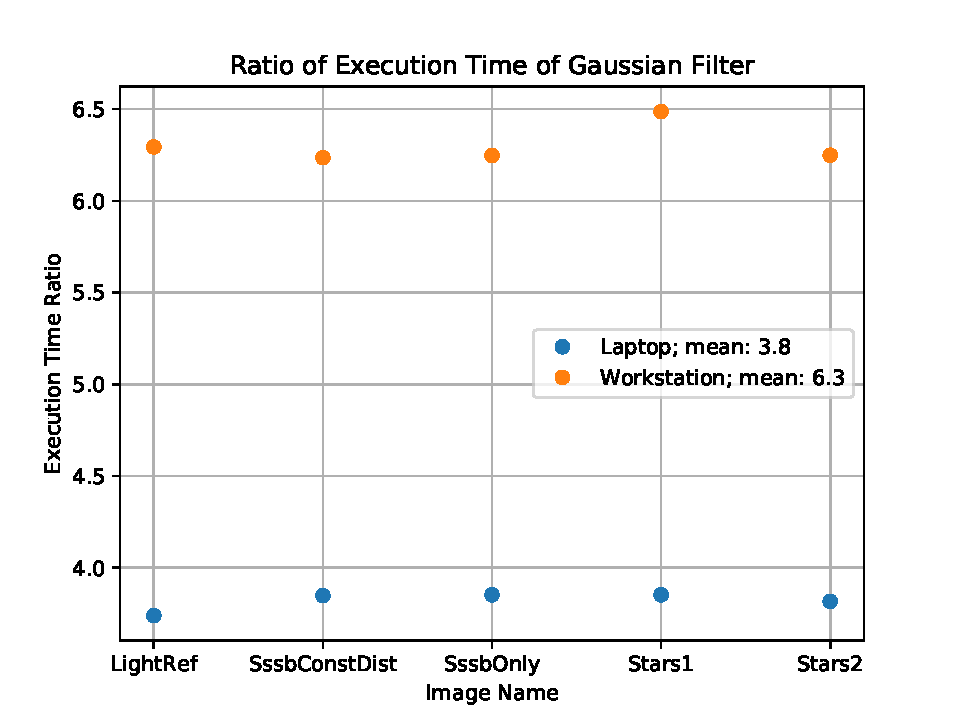
\includegraphics[width=\textwidth]{doc/thesis/0_figures/cv_skimage/Comparison_Gaussian}
        \caption{Gaussian filtering.}
        \label{fig:bm_comparison_gauss}
    \end{subfigure}
    \begin{subfigure}[b]{0.47\textwidth}
        \centering
        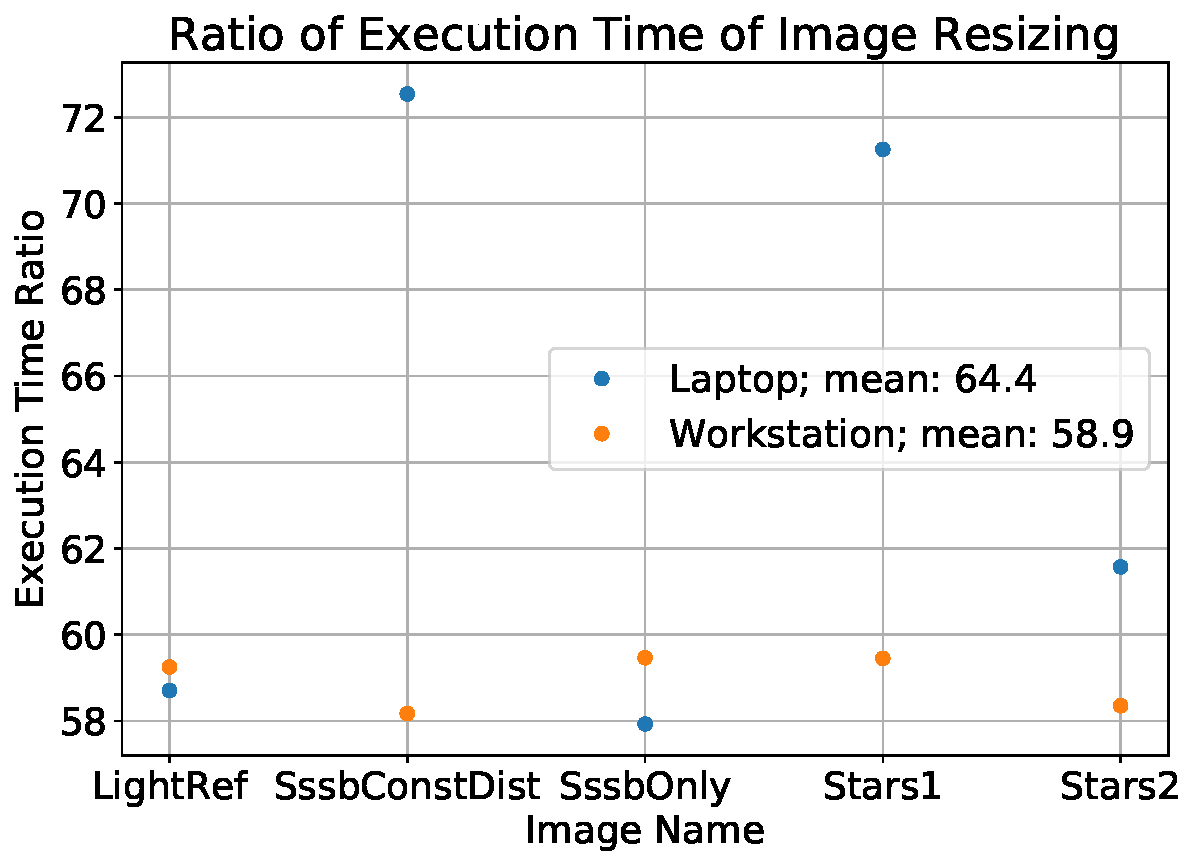
\includegraphics[width=\textwidth]{doc/thesis/0_figures/cv_skimage/Comparison_Resize}
        \caption{Resizing.}
        \label{fig:bm_comparison_res}
    \end{subfigure}
    \caption{Comparison of execution time ratios of Gaussian filtering and resizing five images using OpenCV and \gls{skimage} on two computers. Values $> 1$ correspond to OpenCV being faster. The mean values are given in the legend.}
    \label{fig:bm_comparison}
\end{figure}

For our case, OpenCV has a clear performance advantage over the \gls{skimage} library, hence only OpenCV is being used. In addition to the performance advantages, OpenCV might also be used to replace the OpenEXR dependency in the future, if OpenCV's OpenEXR implementation includes alpha channel support\footnote{A GitHub issue was created at \url{https://github.com/YgabrielsY/sispo/issues/128} that links to the relevant OpenCV GitHub issue.}.

\subsection{Future Developments}
There are several issues left open within the \gls{sispo} software package. First, there is currently no realistic model of spacecraft attitude motion and control implemented. The camera of the simulation environment is perfectly oriented towards the centre of the \gls{sssb}'s nucleus during the entire simulation. Realistic rotation should cover at least two effects, motion blur due to instantaneous rotation velocities of spacecraft and off-centre pointing due to control inaccuracies. Furthermore, it is necessary to include  image distortions such as astigmatism, bokeh, coma, field curvature, glare. Moreover, it is necessary to include a gas and dust environment around the nucleus. From a technical perspective, a proper simulation of the data transmission should be included. For example, a realistic simulation for packet loss. The ultimate goal is to develop a prioritisation algorithm for the images which should prioritise data transmission on packet level.
Moreover, multi-instumrent capability was intended as well as including multiple \gls{sssb}s in the future to allow more complex simulations including e.g. a binary system.
Furthermore, the shader used to create the \gls{sssb} models should be developed further. The interface for it should be included into \gls{sispo} and restricted to values that create reasonable shaped outputs.
An attempt to include a HAPKE model via the synthspace package \url{https://github.com/oknuutti/synthspace} was unsuccessful. However, it would be interesting to compare the results of Blender and the HAPKE model. A HAPKE model is substantially faster while providing less detail though possibly still sufficient for some cases.

THOUGHTS:\\
-default data set, different compression and reconstruction\\
    -compressions: png, jpg2000 quality 1000, jpg2000 quality 500, jpg2000 quality 100, jpg2000 quality 10\\
-different trajectories: default : 400 km, 100km, 1000km\\
-different lighting situations\\
-different models 100m, 1km, 10km


\clearpage
\section{Results} \label{sec:results}

\begin{table}[htpb]
\caption{Simulation parameters}
\label{tab:sim_params}
\begin{tabular}{l|lll}
ID      & \gls{sssb} Size \SI{}{\kilo\meter} & Encounter Distance \SI{}{\kilo\meter} & Compression Method      \\
Default & 1                                                                                                        & 400                                                                                          & png                     \\
1       & 1                                                                                                        & 400                                                                                          & jpeg2000: quality 1000  \\
2       & 1                                                                                                        & 400                                                                                          & jpeg2000: quality 100   \\
3       & 1                                                                                                        & 400                                                                                          & jpeg2000: quality 10    \\
4       & 1                                                                                                        & 100                                                                                          & png                     \\
5       & 1                                                                                                        & 100                                                                                          & jpeg2000 : quality 1000 \\
6       & 1                                                                                                        & 100                                                                                          & jpeg2000: quality 100   \\
7       & 1                                                                                                        & 100                                                                                          & jpeg200: quality 10     \\
8       & 1                                                                                                        & 1000                                                                                         & png                     \\
9       & 1                                                                                                        & 1000                                                                                         & jpeg2000 : quality 1000 \\
10      & 1                                                                                                        & 1000                                                                                         & jpeg2000 : quality 100  \\
11      & 1                                                                                                        & 1000                                                                                         & jpeg2000 : quality 10   \\
12      & 10                                                                                                       & 400                                                                                          & png                     \\
13      & 10                                                                                                       & 400                                                                                          & jpeg2000 : quality 1000 \\
14      & 10                                                                                                       & 400                                                                                          & jpeg2000 : quality 100  \\
15      & 10                                                                                                       & 400                                                                                          & jpeg2000 : quality 10   \\
16      & 0.1                                                                                                      & 400                                                                                          & png                     \\
17      & 0.1                                                                                                      & 400                                                                                          & jpeg2000 : quality 1000 \\
18      & 0.1                                                                                                      & 400                                                                                          & jpeg2000 : quality 100  \\
19      & 0.1                                                                                                      & 400                                                                                          & jpeg2000 : quality 10  
\end{tabular}
\end{table}

% \clearpage
% \section{Conclusion} \label{sec:conclusion}
\subsection{Summary}
A first implementation for simulating a \gls{sssb} flyby mission could be created. It is capable of rendering images, compressing and decompressing these images and reconstructing a textured \gls{3d} model.
The rendering output of \gls{sispo} better resembles asteroids than comets.

It was possible to show the influence of compression on images. However, quantifying image quality solely on the number of reconstructed points

\subsection{Future Developments}
There are several issues left open within the \gls{sispo} software package. First, there is currently no realistic model of spacecraft attitude motion and control implemented. The camera of the simulation environment is perfectly oriented towards the centre of the \gls{sssb}'s nucleus during the entire simulation. Realistic rotation should cover at least two effects, motion blur due to instantaneous rotation velocities of spacecraft and off-centre pointing due to control inaccuracies. Furthermore, it is necessary to include  image distortions such as astigmatism, bokeh, coma, field curvature, glare.

Currently, \gls{sispo} assumes that an instrument always has \gls{rgb} channels. Since many \gls{ccd}s used in deep space are only \gls{bw} cameras, a possibility to choose either \gls{rgb} or \gls{bw} should be implemented.

Moreover, it is necessary to include a gas and dust environment around the nucleus. From a technical perspective, a proper simulation of the data transmission should be included. For example, a realistic simulation for packet loss. The ultimate goal is to develop a prioritisation algorithm for the images which should prioritise data transmission on packet level.
Moreover, multi-instrument capability was intended as well as including multiple \gls{sssb}s in the future to allow more complex simulations including e.g. a binary system.

Furthermore, the shader used to create the \gls{sssb} models should be developed further. The interface for it should be included into \gls{sispo} and restricted to values that create reasonable shaped outputs. Additionally, the shader should also represent comet surfaces better. Furthermore, since most of the execution time is spent rendering, the shader should be developed to be less computationally heavy.

An attempt to include a HAPKE model via the synthspace package \url{https://github.com/oknuutti/synthspace} was unsuccessful. However, it would be interesting to compare the results of Blender and the HAPKE model. A HAPKE model is substantially faster while being less accurate though possibly still sufficient for some cases.

To improve computational performance and make image compression and possible data transmission more realistic, image cropping should be added. A substantial part of an image far from a nucleus is black which could be cropped away to reduce the amount of data for the computation and the system itself.

\clearpage

\thesisbibliography
\printbibliography

%% Appendices
%% If you don't have appendices, remove \clearpage and \thesisappendix below.
\clearpage

\thesisappendix
\pagestyle{empty}
\section{Esimerkki liitteest\"a\label{LiiteA}}
Liitteet eiv\"at ole opinn\"aytteen kannalta v\"altt\"am\"att\"omi\"a ja 
opinn\"aytteen tekij\"an on 
kirjoittamaan ryhtyess\"a\"an hyv\"a ajatella p\"arj\"a\"av\"ans\"a ilman liitteit\"a.
Kokemattomat kirjoittajat, jotka ovat huolissaan
tekstiosan pituudesta, paisuttavat turhan 
helposti liitteit\"a pit\"a\"akseen tekstiosan pituuden annetuissa rajoissa.
T\"all\"a tavalla ei synny hyv\"a\"a opinn\"aytett\"a.   

Liite on itsen\"ainen kokonaisuus, vaikka se t\"aydent\"a\"akin tekstiosaa.
Liite ei siten ole pelkk\"a listaus, kuva tai taulukko, vaan 
liitteess\"a selitet\"a\"an aina sis\"all\"on laatu ja tarkoitus. 

Liitteeseen voi laittaa esimerkiksi listauksia. Alla on 
listausesimerkki t\"am\"an liitteen luomisesta. 

%% Verbatim-ymp\"arist\"o ei muotoile tai tavuta teksti\"a. Fontti on monospace.
%% Verbatim-ymp\"arist\"on sis\"all\"a annettuja komentoja ei LaTeX k\"asittele. 
%% Vasta \end{verbatim}-komennon j\"alkeen jatketaan k\"asittely\"a.
\begin{verbatim}
	\clearpage
	\appendix
	\addcontentsline{toc}{section}{Liite A}
	\section*{Liite A}
	...
	\thispagestyle{empty}
	...
	teksti\"a
	...
	\clearpage
\end{verbatim}

Kaavojen numerointi muodostaa liitteiss\"a oman kokonaisuutensa:
\begin{align}
d \wedge A &= F, \label{liitekaava1}\\
d \wedge F &= 0. \label{liitekaava2}
\end{align}


\clearpage
\section{Shader Node Network} \label{sec:shader_node}

\begin{figure}[htb]
    \centering
    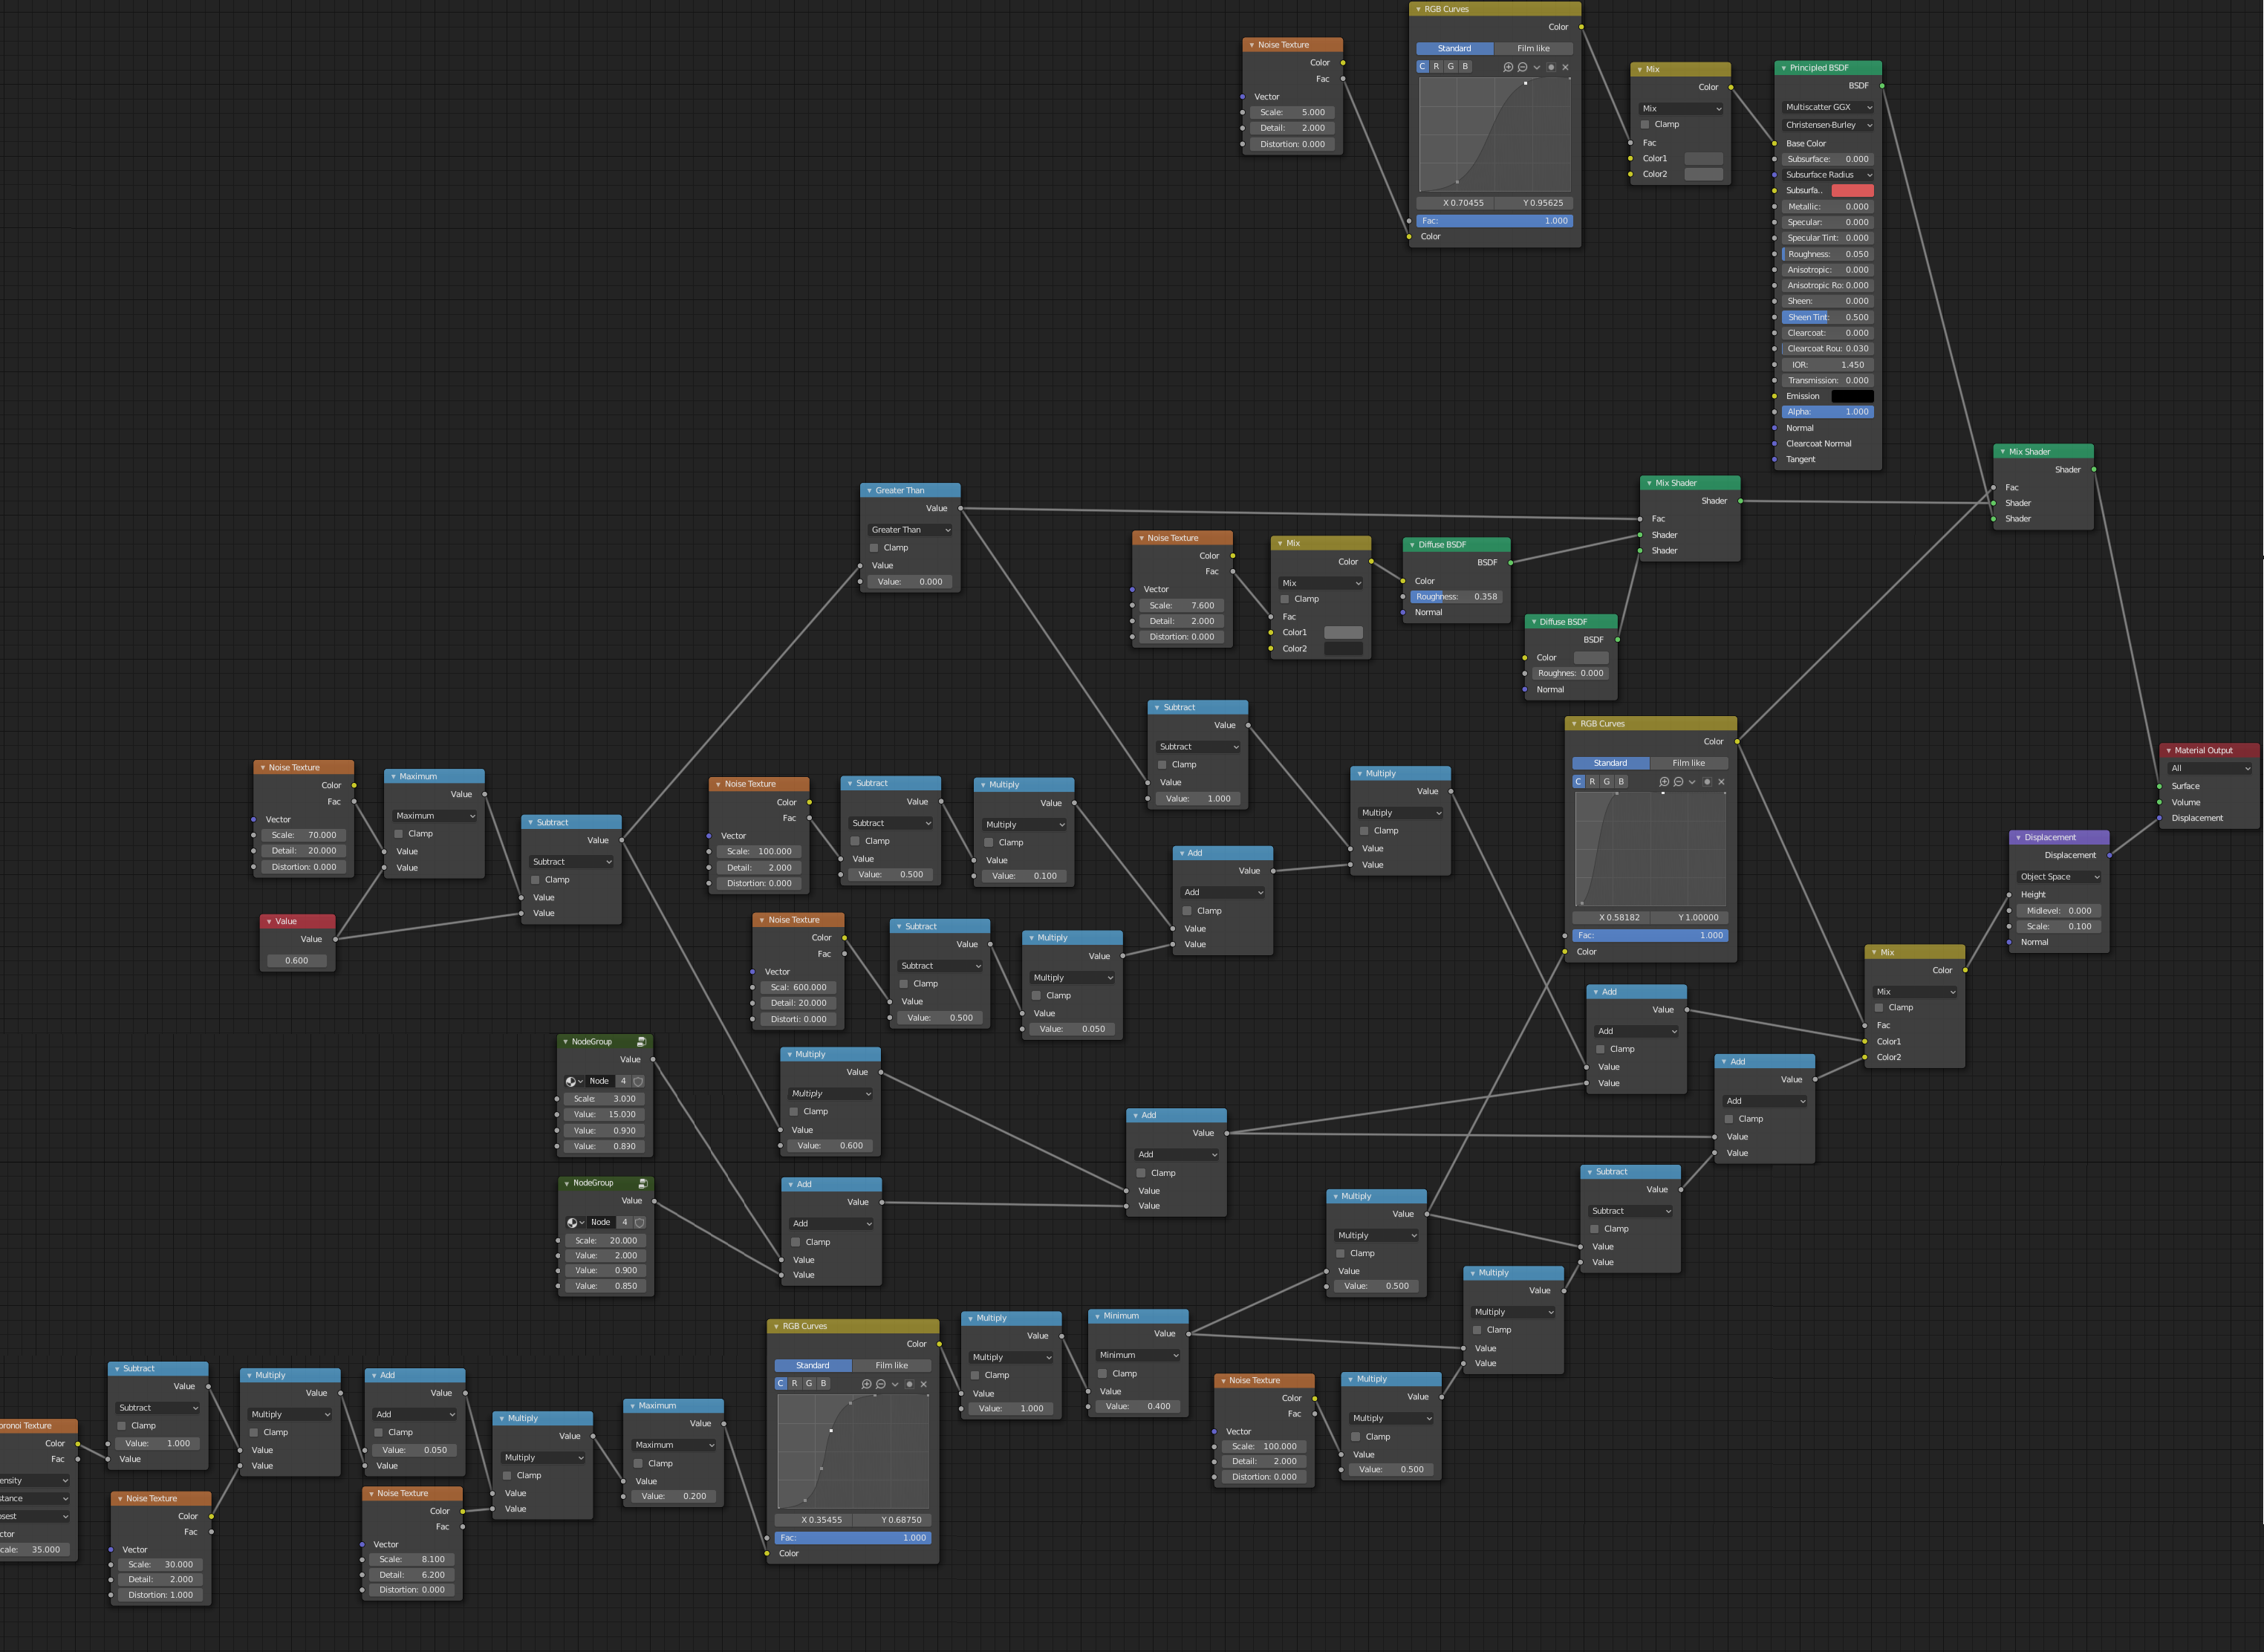
\includegraphics[height=.97\textwidth, angle=90]{doc/thesis/0_figures/procedural_terrain/node_network_highres.png}
    \caption{High resolution image of the shader node network used in \gls{sispo}.}
    \label{fig:node_highres}
\end{figure}


%\section{Toinen esimerkki liitteest\"a\label{LiiteB}}
%% Liitteiden kaavat, taulukot ja kuvat numeroidaan omana kokonaisuutenaan
%%
%% Equations, tables and figures have their own numbering in Appendices
%\renewcommand{\theequation}{B\arabic{equation}}
%\setcounter{equation}{0}  
%\renewcommand{\thefigure}{B\arabic{figure}}
%\setcounter{figure}{0}
%\renewcommand{\thetable}{B\arabic{table}}
%\setcounter{table}{0}

% Liitteiss\"a voi my\"os olla kuvia, jotka
% eiv\"at sovi leip\"atekstin joukkoon:
% %% Ymp\"arist\"on figure parametrit htb pakottavat
% %% kuvan t\"ah\"an, eik\"a LaTeX yrit\"a siirrell\"a niit\"a
% %% hyv\"aksi katsomaansa paikkaan. 
% %% Ymp\"arist\"o\"a center voi k\"aytt\"a\"a \centering-
% %% komennon sijaan
% %%
% %% Example of a figure, note the use of htb parameters which force
% %% the figure to be inserted here
% \begin{figure}[htb]
% \begin{center}
% 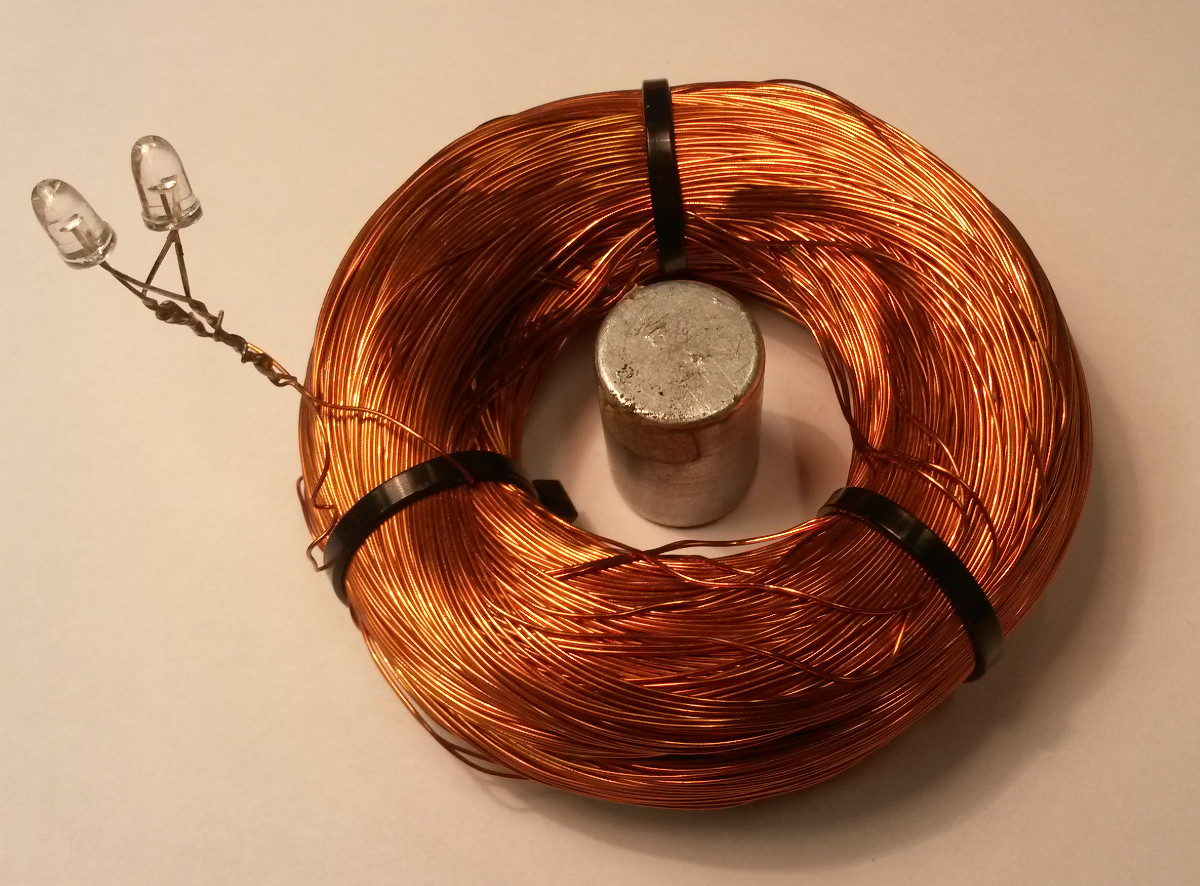
\includegraphics[height=8cm]{doc/thesis/0_figures/ledspole.jpg}
% \end{center}
% \caption{Kuvateksti, jossa on liitteen numerointi}
% \label{liitekuva}
% \end{figure}
% %%
% Liitteiden taulukoiden numerointi on kuvien ja kaavojen kaltainen:
% \begin{table}[htb]
% \caption{Taulukon kuvateksti.}
% \label{liitetaulukko}
% \begin{center}
% \fbox{
% \begin{tabular}{lp{0.5\linewidth}}
% 9.00--9.55  & K\"aytett\"avyystestauksen tiedotustilaisuus (osanottajat
% ovat saaneet s\"ahk\"opostitse valmistautumisteht\"av\"at, joten tiedotustilaisuus
% voidaan pit\"a\"a lyhyen\"a).\\
% 9.55--10.00 & Testausalueelle siirtyminen
% \end{tabular}}
% \end{center}
% \end{table}
% Kaavojen numerointi muodostaa liitteiss\"a oman kokonaisuutensa:
% \begin{align}
% T_{ik} &= -p g_{ik} + w u_i u_k + \tau_{ik},  \label{liitekaava3} \\
% n_i    &= n u_i + v_i.                      \label{liitekaava4}
% \end{align}

% \clearpage
% \section{Image Set for Image Processing Benchmark} \label{sec:app_cvskimage}


\begin{figure}[htb]
    \begin{center}
        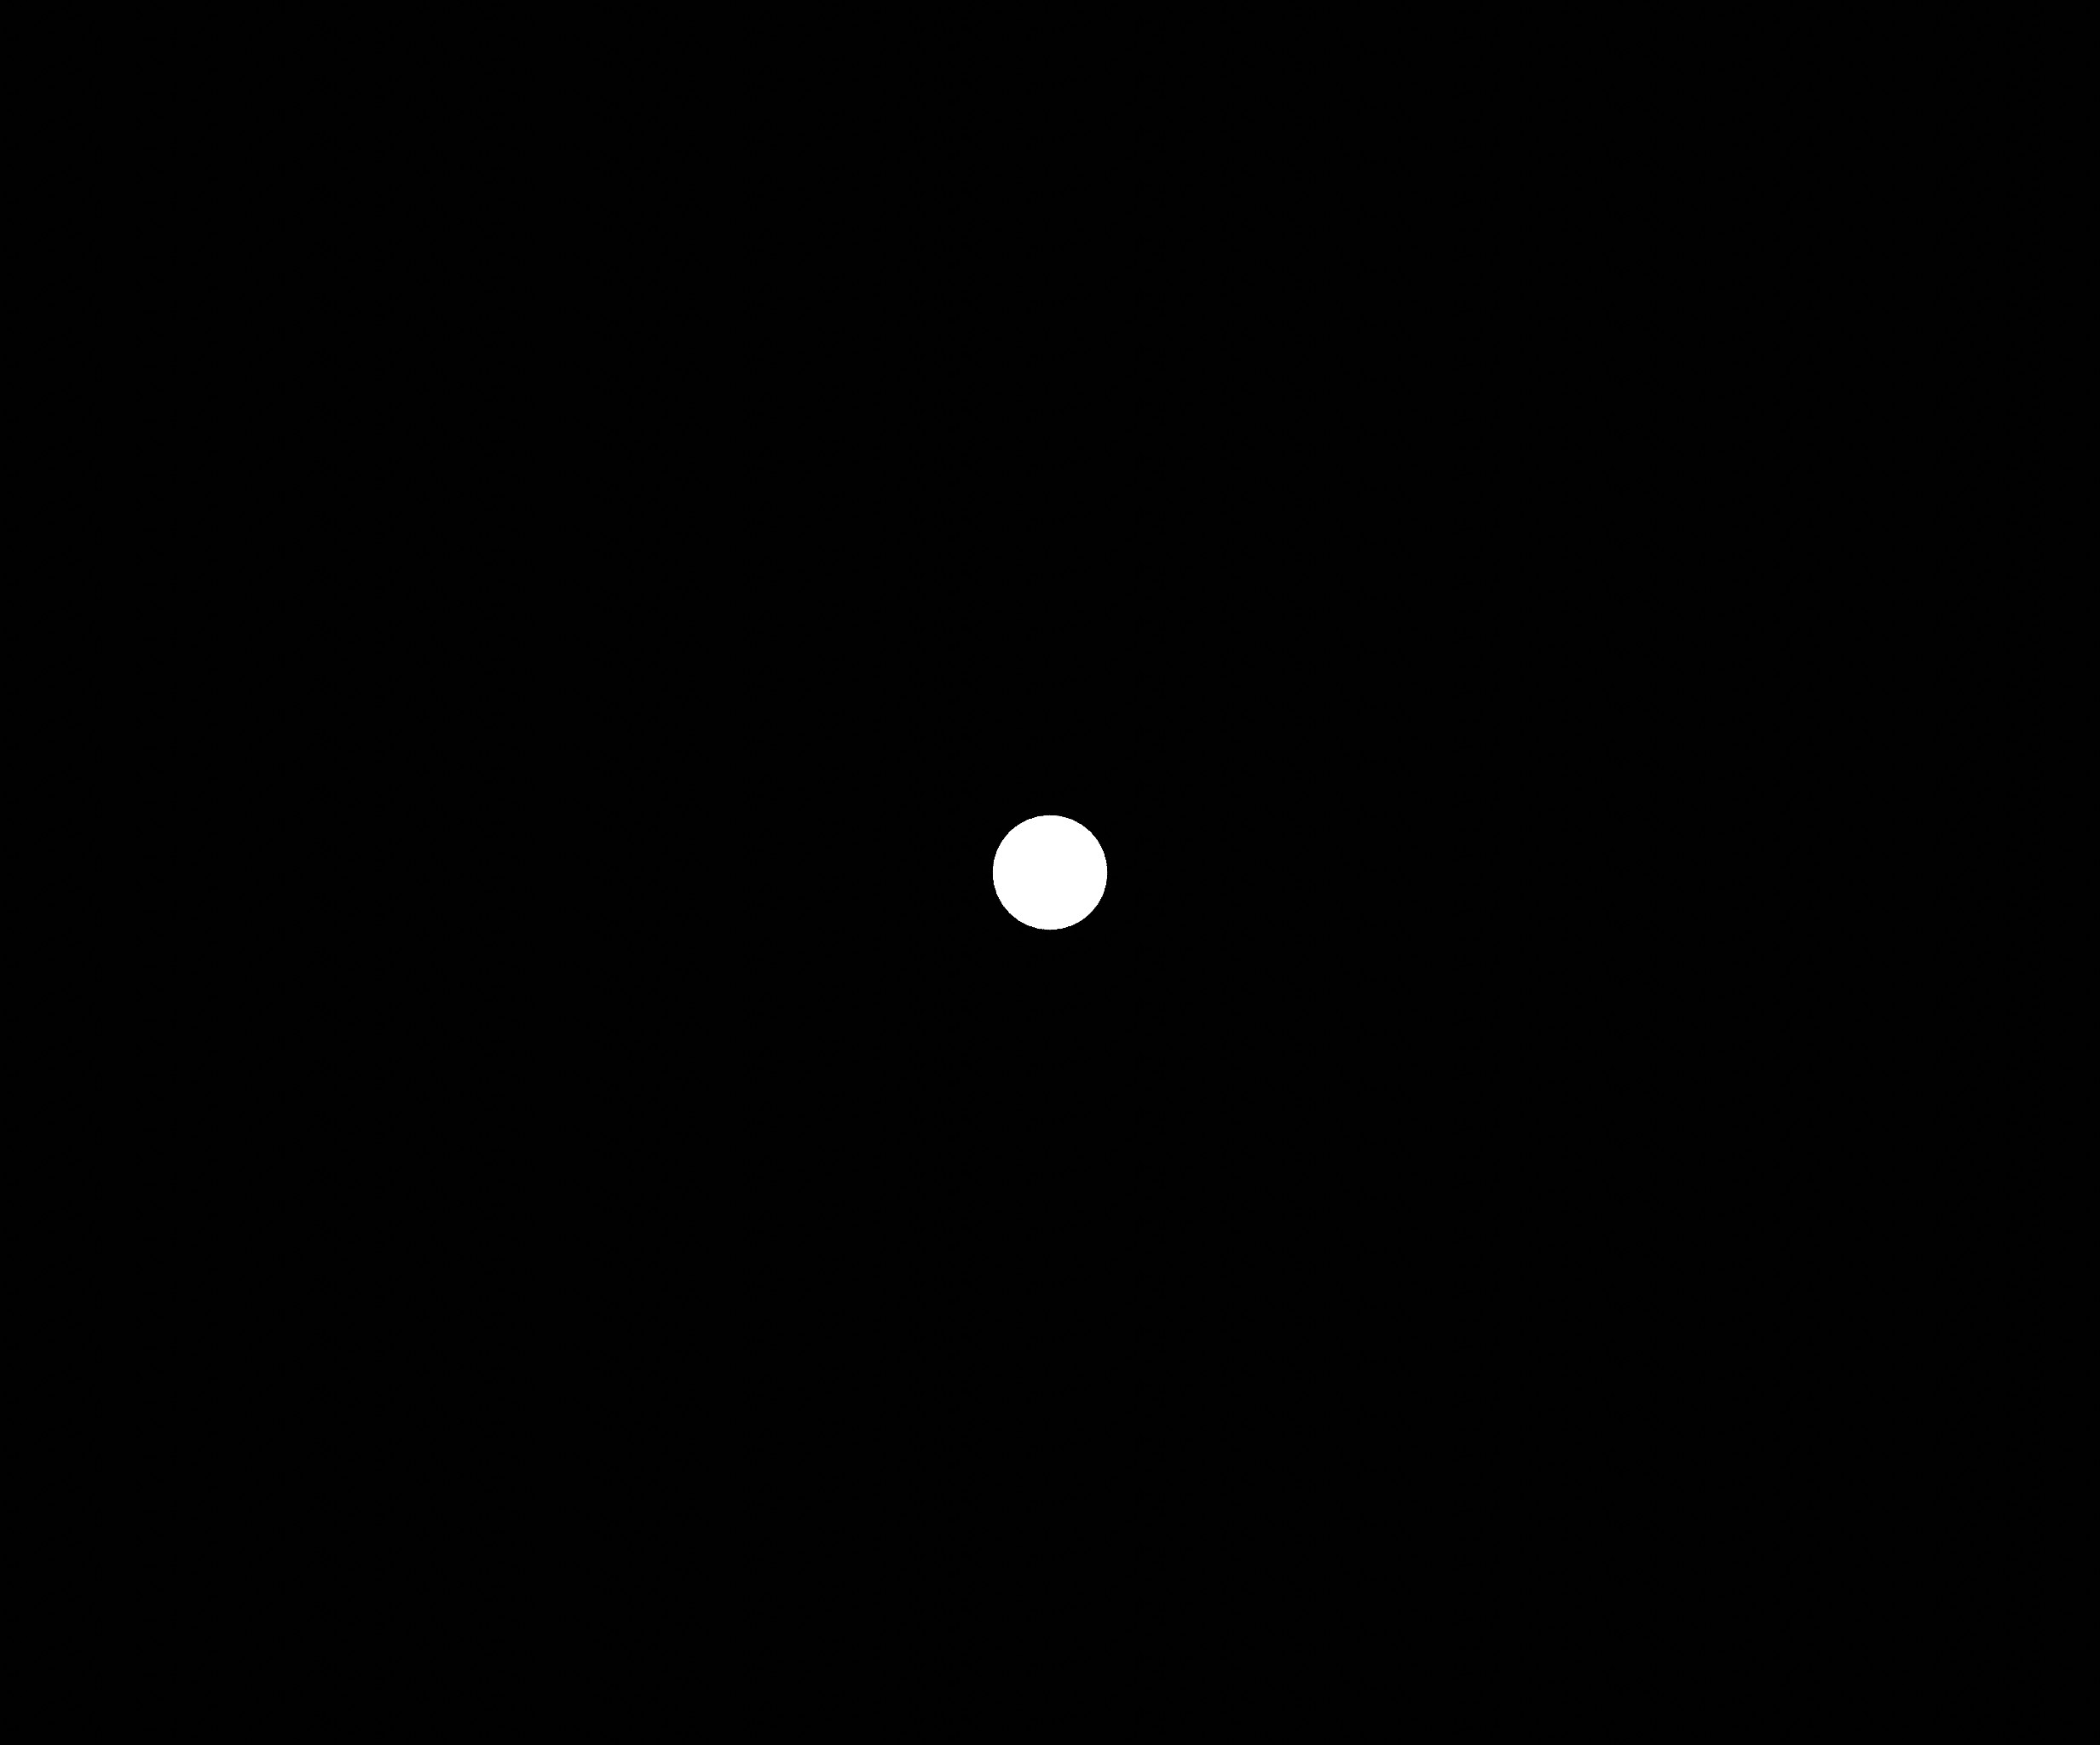
\includegraphics[height=8cm]{doc/thesis/0_figures/cv_skimage/LightRef_2017-08-15T115851-679000.jpg}
    \end{center}
    \caption{LightRef image used in benchmark.}
    \label{fig:bm_light_ref}
\end{figure}

\begin{figure}[htb]
    \begin{center}
        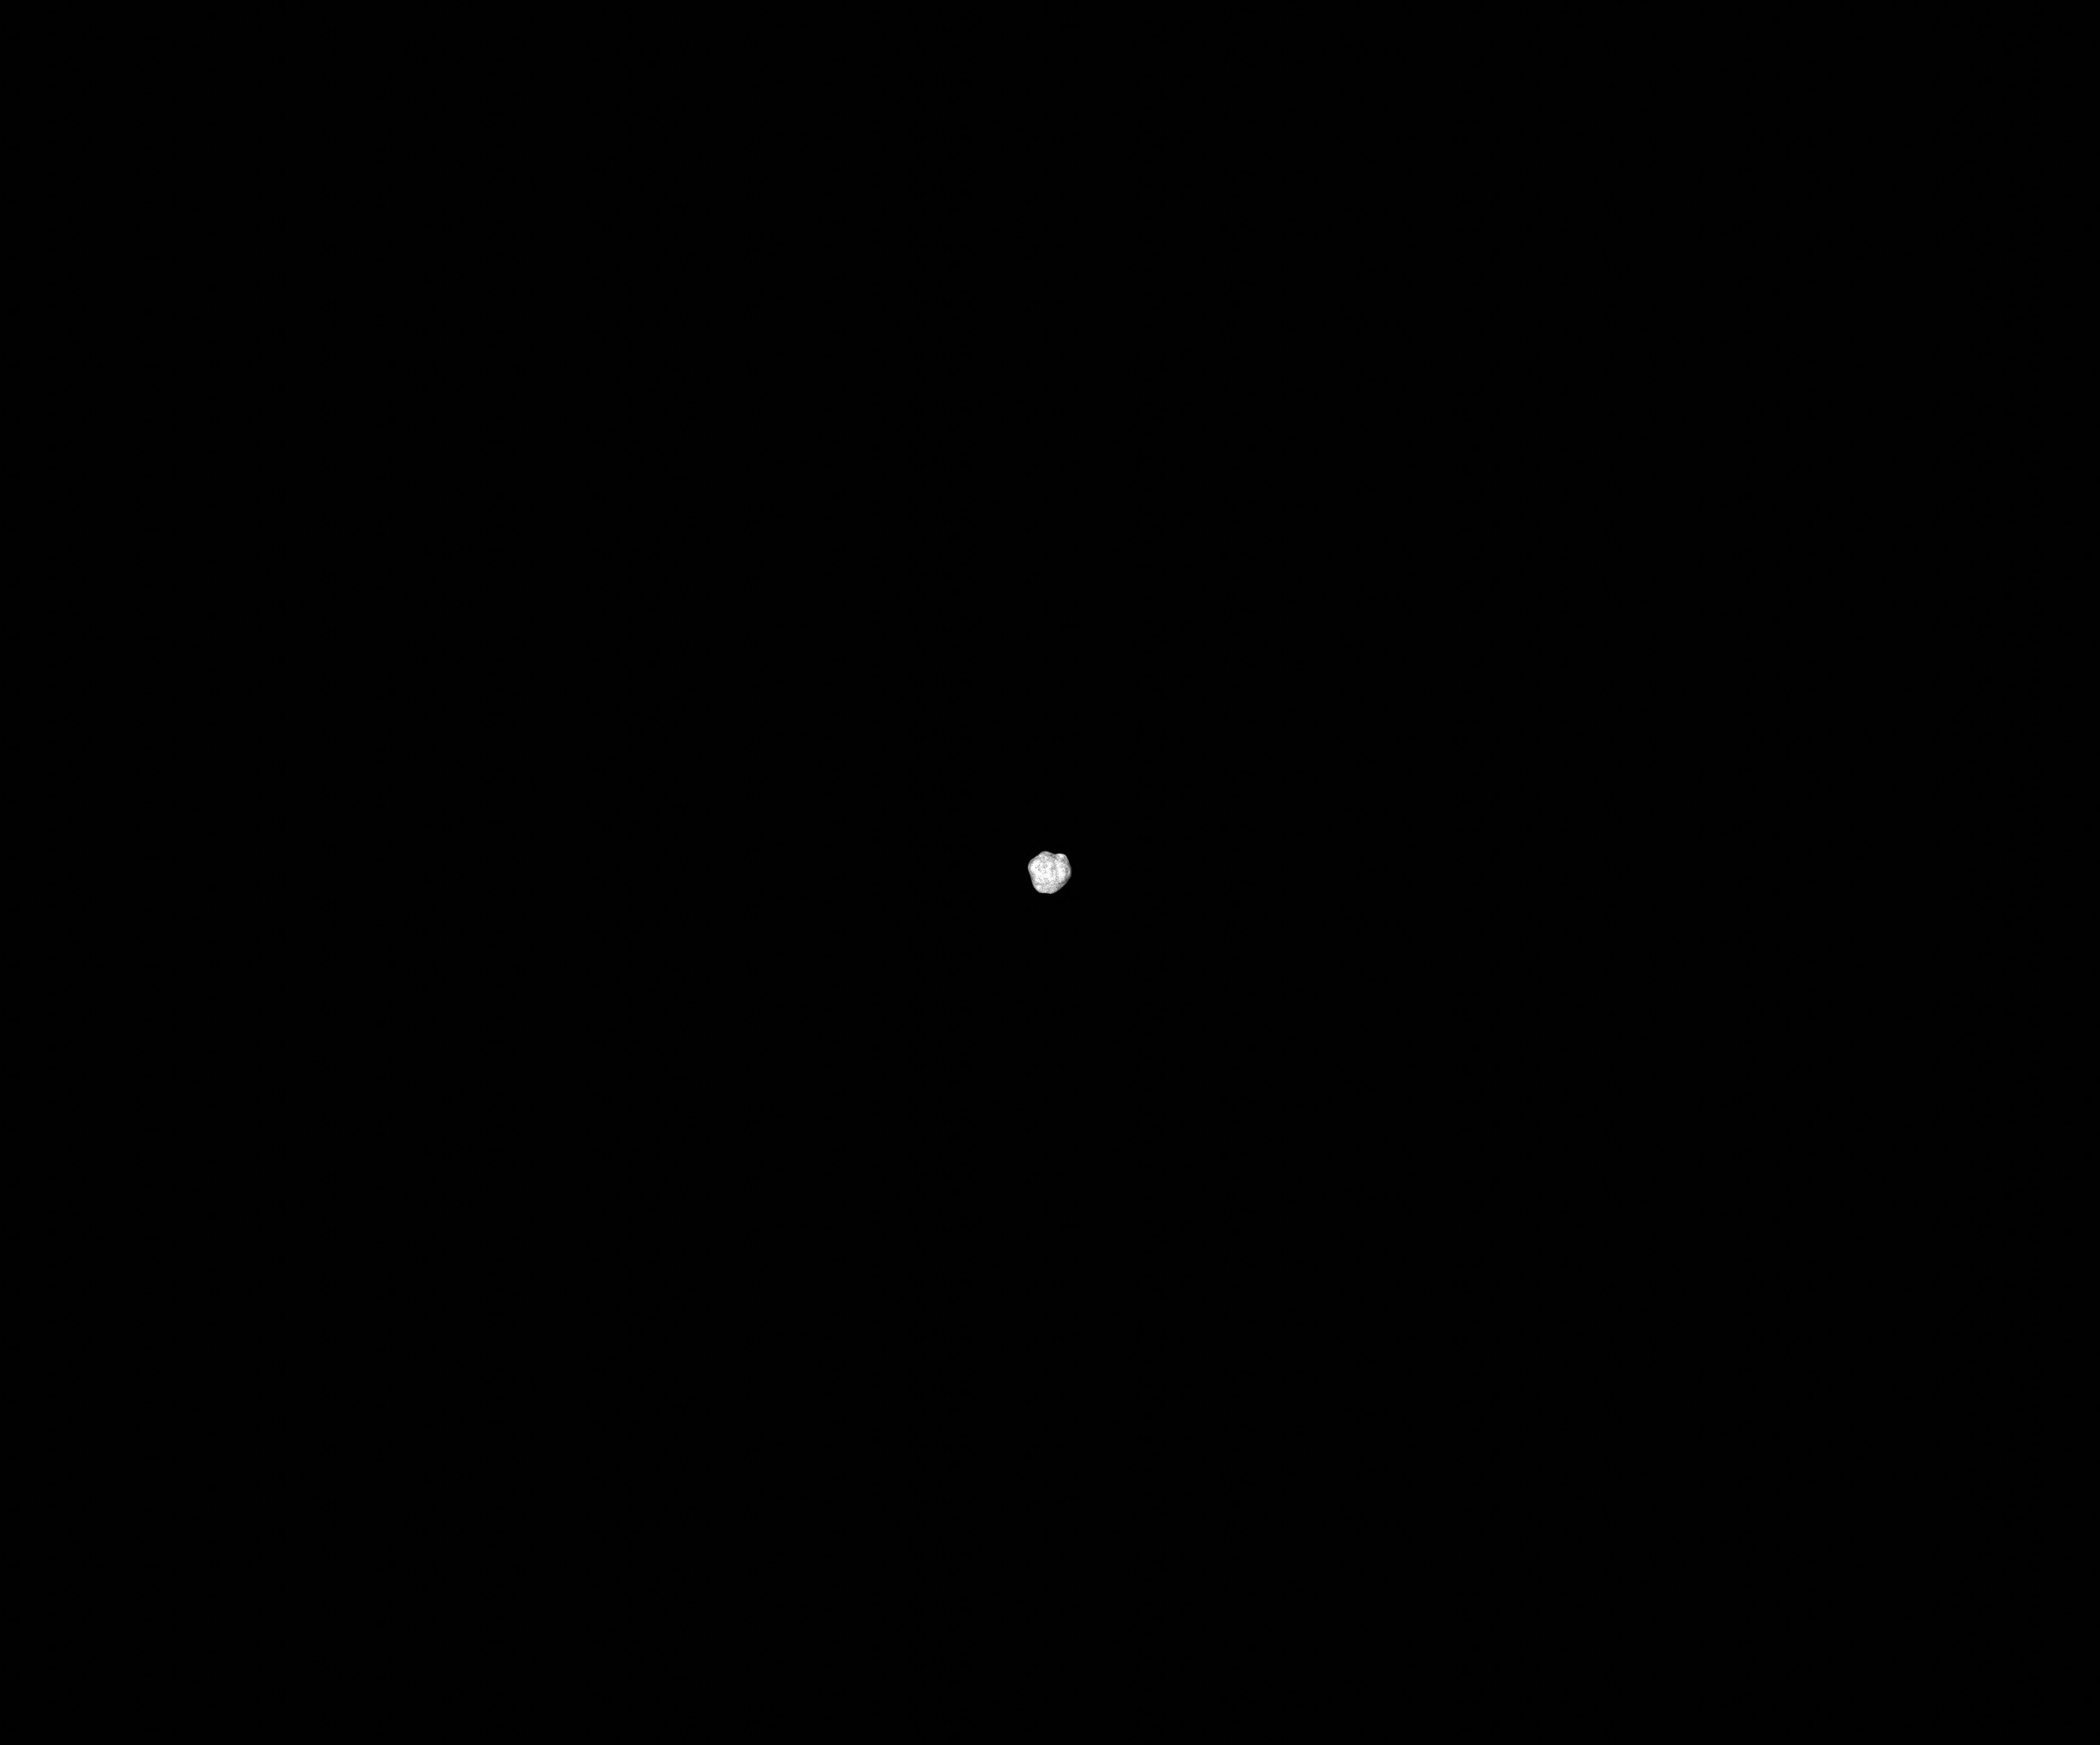
\includegraphics[height=8cm]{doc/thesis/0_figures/cv_skimage/SssbConstDist_2017-08-15T115851-679000.jpg}
    \end{center}
    \caption{SssbConstDist image used in benchmark.}
    \label{fig:bm_sssbconstdist}
\end{figure}

\begin{figure}[htb]
    \begin{center}
        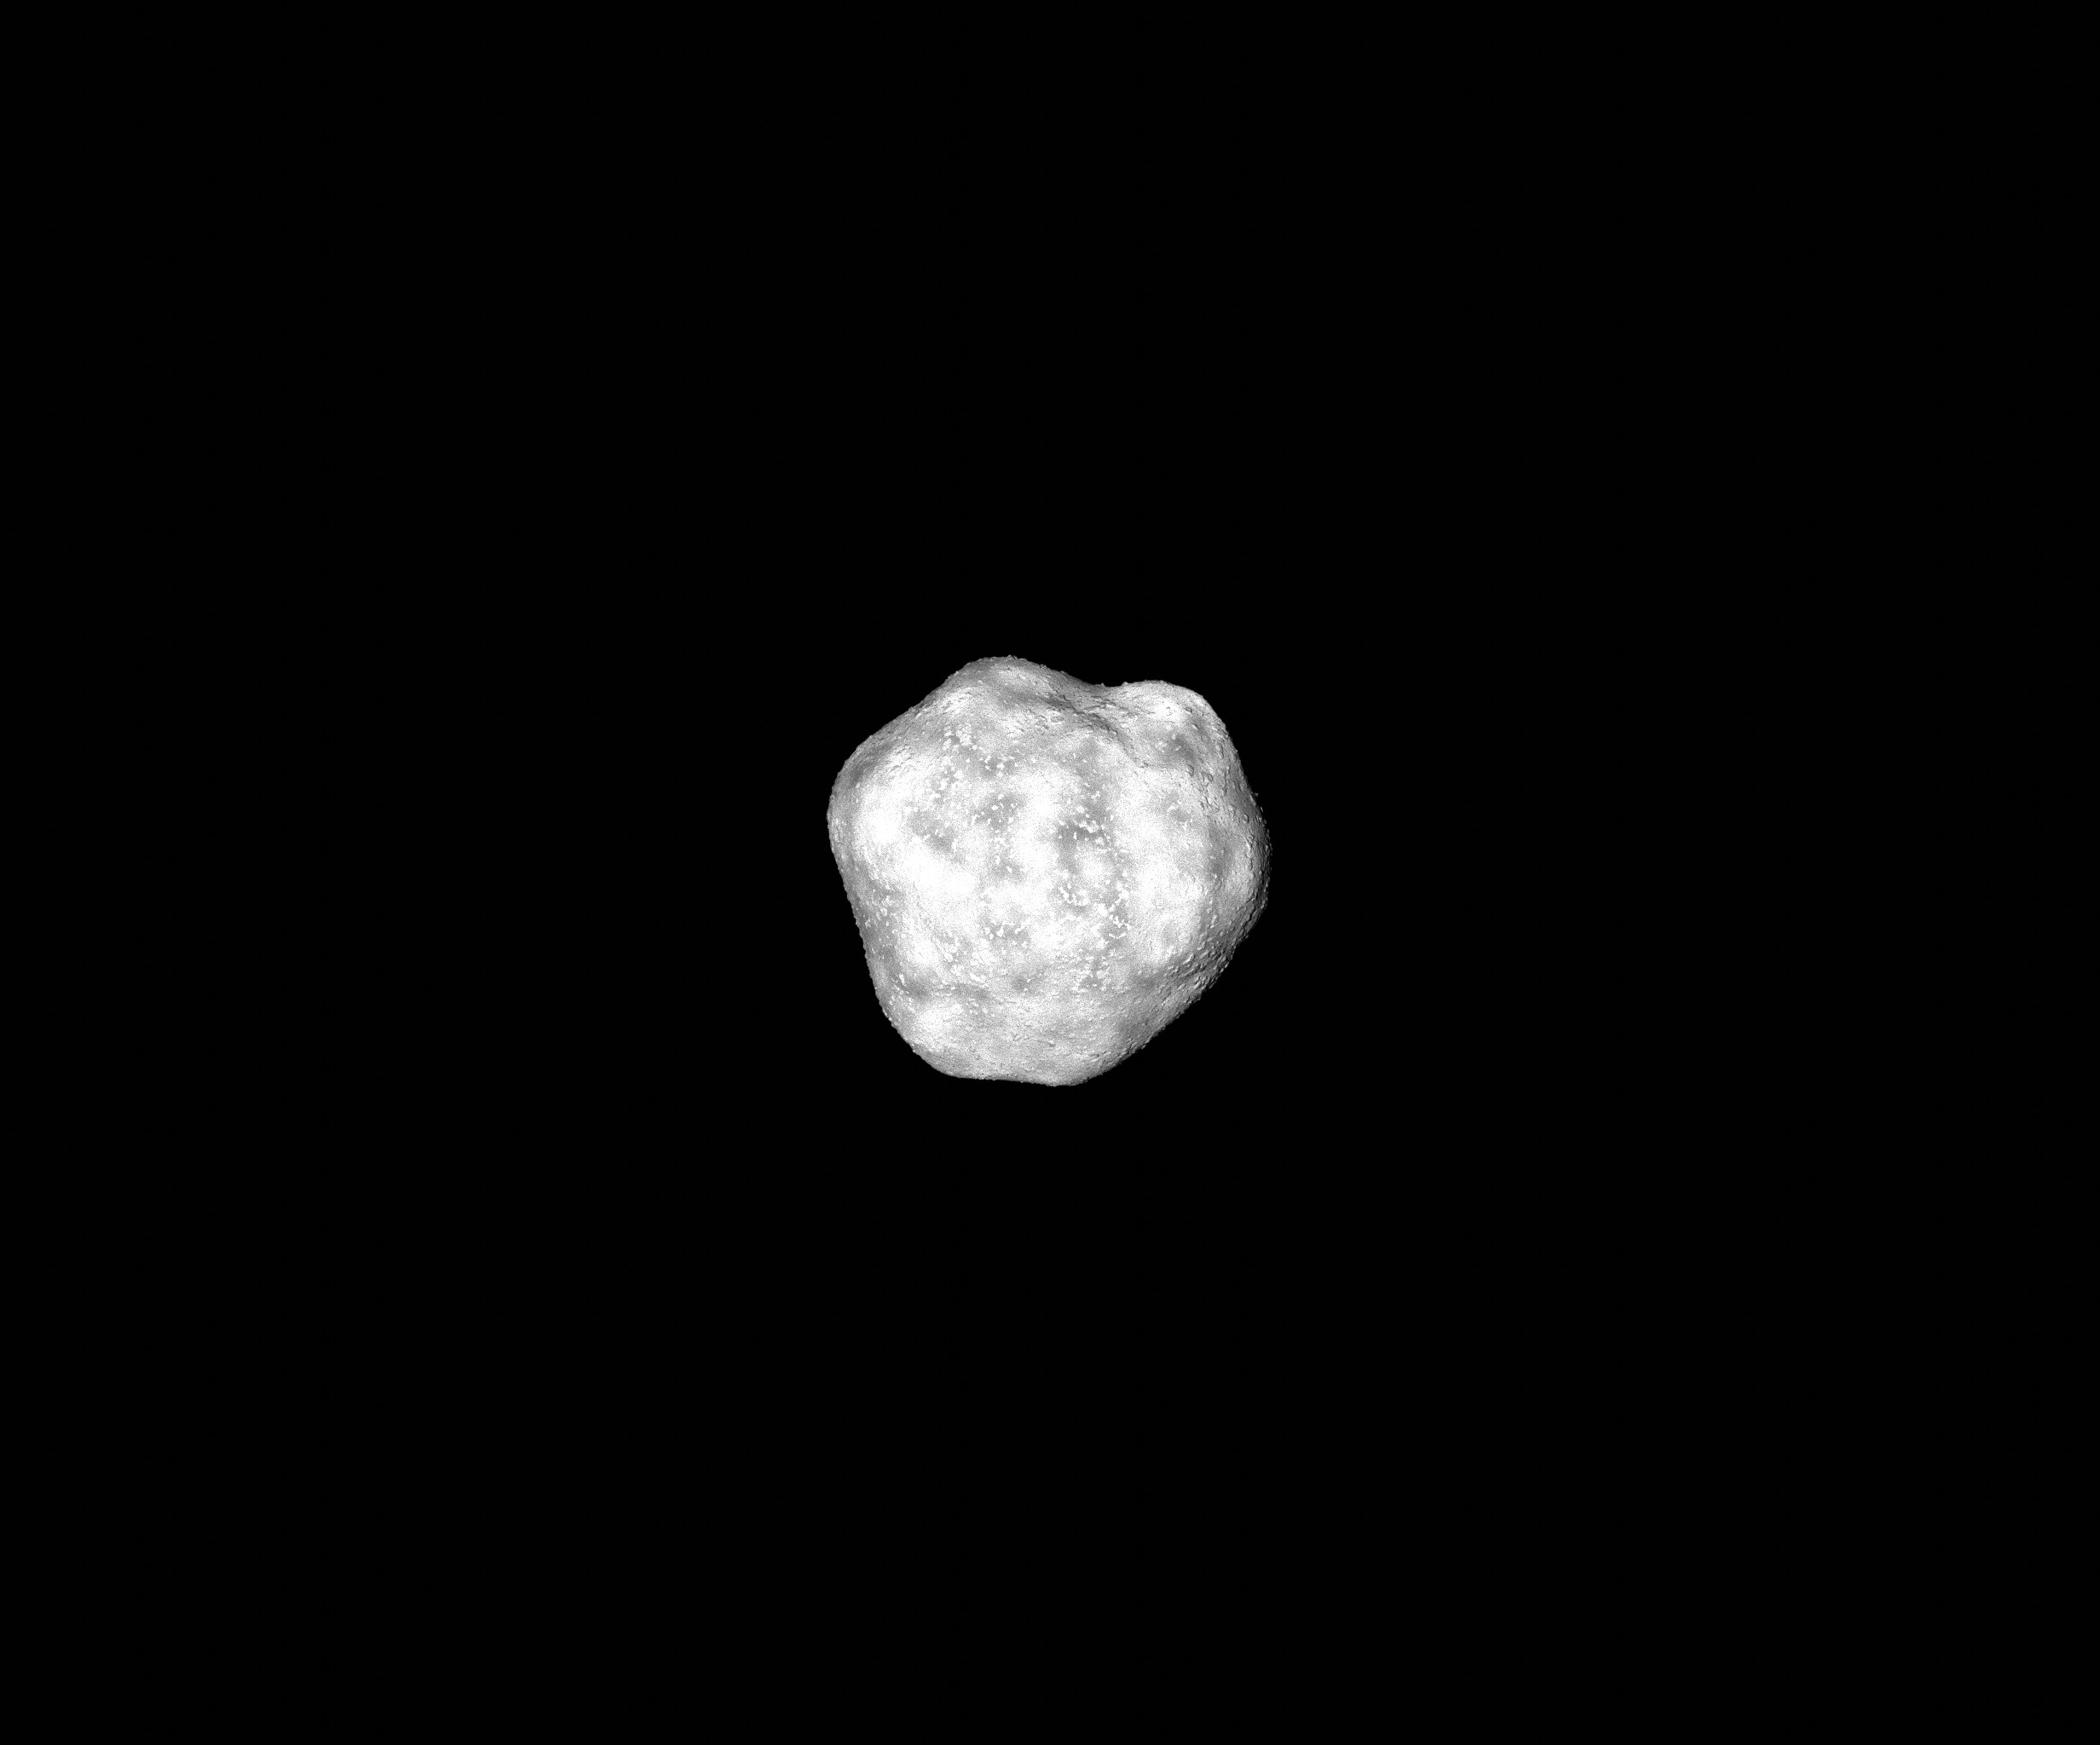
\includegraphics[height=8cm]{doc/thesis/0_figures/cv_skimage/SssbOnly_2017-08-15T115851-679000.jpg}
    \end{center}
    \caption{SssbOnly image used in benchmark.}
    \label{fig:bm_sssbonly}
\end{figure}

\begin{figure}[htb]
    \begin{center}
        
\includegraphics[height=8cm]{doc/thesis/0_figures/cv_skimage/Stars_2017-08-15T115841-334000.png}
    \end{center}
    \caption{Stars1 image used in benchmark. The image is based on 1804 stars.}
    \label{fig:bm_stars1}
\end{figure}

\begin{figure}[htb]
    \begin{center}
        
\includegraphics[height=8cm]{doc/thesis/0_figures/cv_skimage/Stars_2017-08-15T115857-362000.png}
    \end{center}
    \caption{Stars2 image used in benchmark. The image is based on 51338 stars.}
    \label{fig:bm_stars2}
\end{figure}

Figures \ref{fig:bm_light_ref} through \ref{fig:bm_stars2} are the images used in the benchmark. Their names are given in the respective caption.

\begin{figure}[htb]
    \begin{center}
        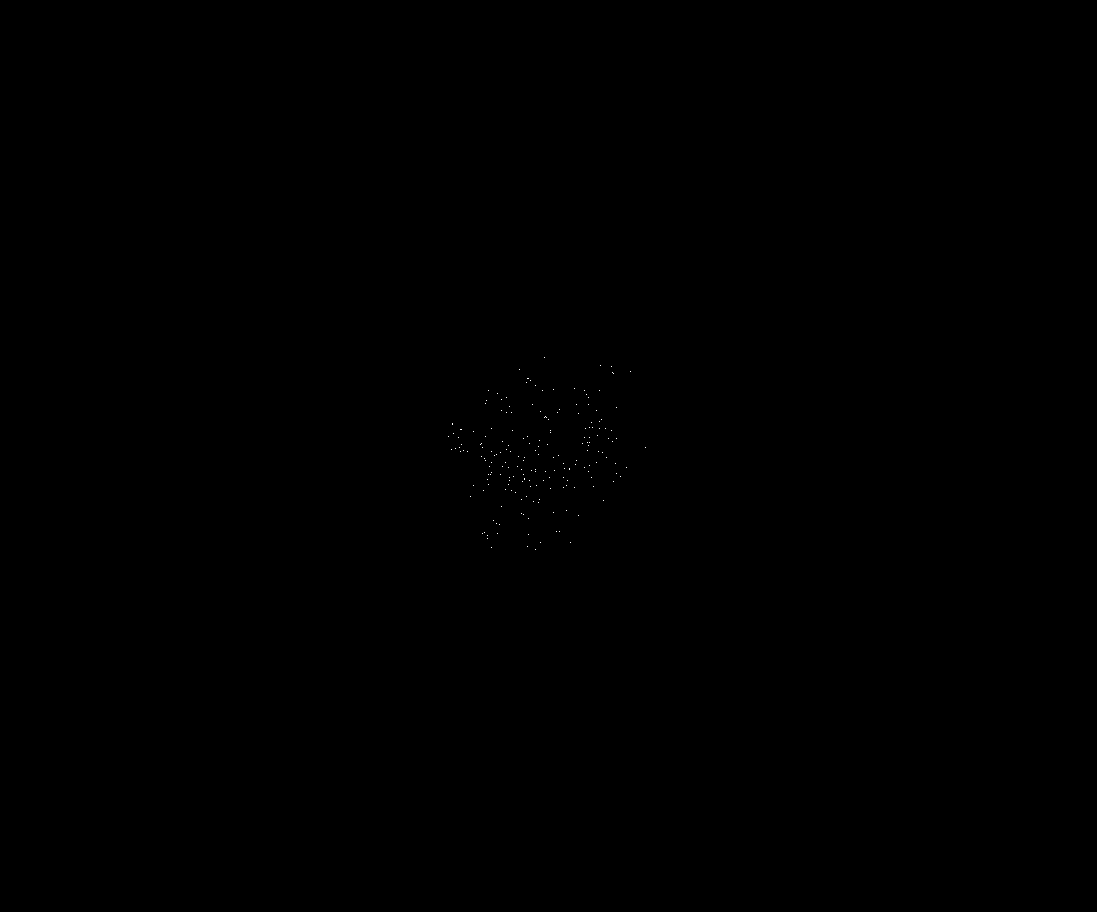
\includegraphics[height=8cm]{doc/thesis/0_figures/cv_skimage/diff_laptop.png}
    \end{center}
    \caption{Difference between \gls{skimage} and OpenCV Gaussian filtered SssbOnly image of the laptop.}
    \label{fig:bm_diff_laptop}
\end{figure}

\begin{figure}[htb]
    \begin{center}
        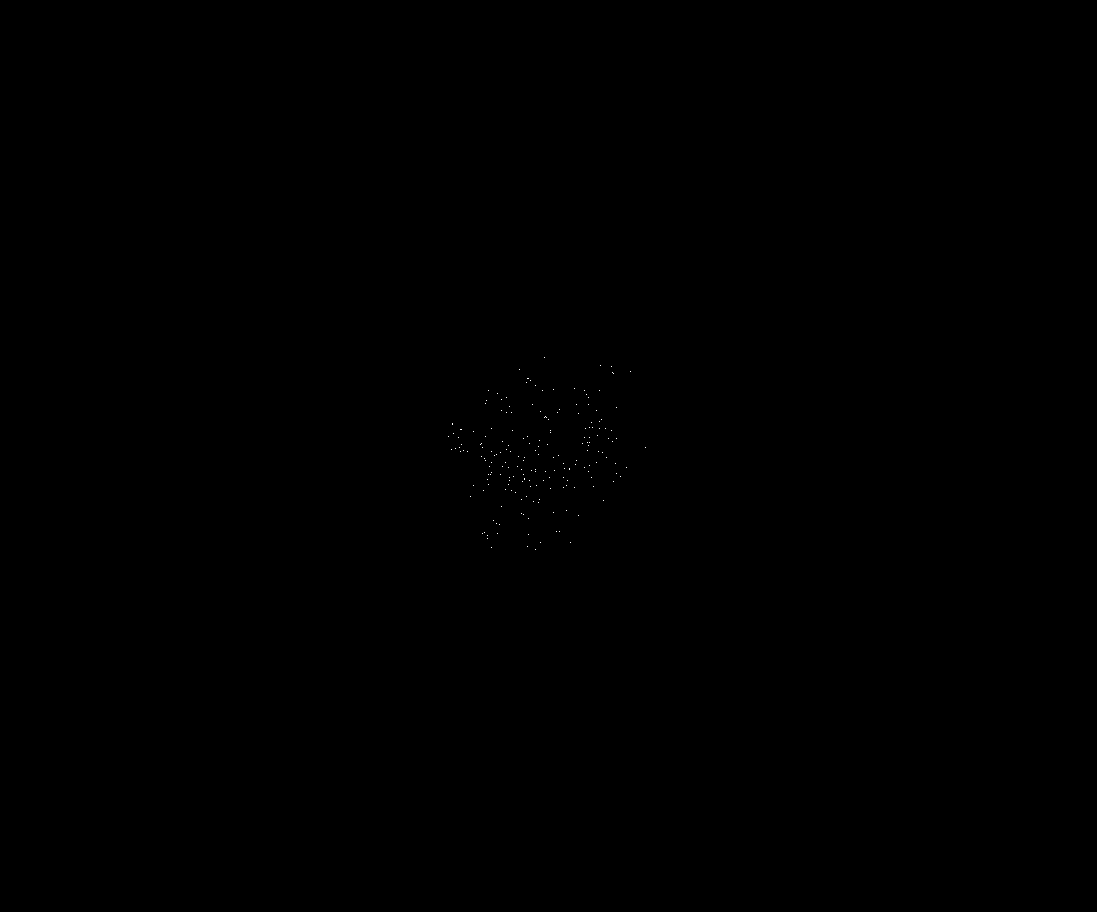
\includegraphics[height=8cm]{doc/thesis/0_figures/cv_skimage/diff_workstation.png}
    \end{center}
    \caption{Difference between \gls{skimage} and OpenCV Gaussian filtered SssbOnly image of the workstation.}
    \label{fig:bm_diff_workstation}
\end{figure}

Figures \ref{fig:bm_diff_laptop} and \ref{fig:bm_diff_workstation} show the difference of the SssbOnly image from the benchmark on the two different computers. Only a small fraction of pixels differ. As discussed previously, the maximum absolute difference is on the order of \SI{1e-6}{}, corresponding to the brightest point in each image. 

% \clearpage
% \section{Difference Images} \label{sec:image_differences}

\begin{figure}[htb]
    \centering
        \begin{subfigure}[b]{0.42\textwidth}
            \centering
            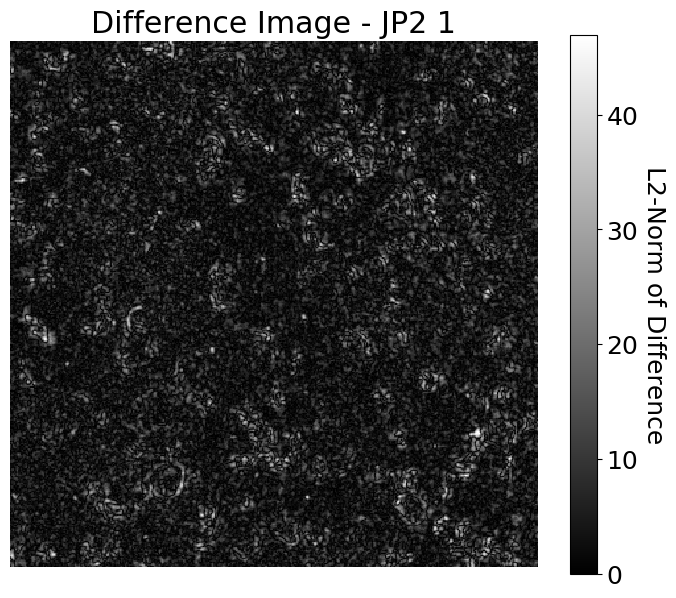
\includegraphics[width=\textwidth]{doc/thesis/0_figures/compare_quality/set1/jp2_1_center_diff_heatmap_rel.png}
            \caption{\gls{jp2} quality 1.}
            \label{fig:img_quality_center_heatmap_rel_1}
        \end{subfigure}
        \begin{subfigure}[b]{0.42\textwidth}
            \centering
            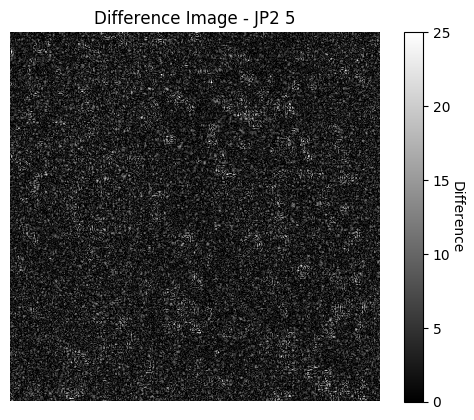
\includegraphics[width=\textwidth]{doc/thesis/0_figures/compare_quality/set1/jp2_5_center_diff_heatmap_rel.png}
            \caption{\gls{jp2} quality 5.}
            \label{fig:img_quality_center_heatmap_rel_5}
        \end{subfigure}
        \\
        \begin{subfigure}[b]{0.42\textwidth}
            \centering
            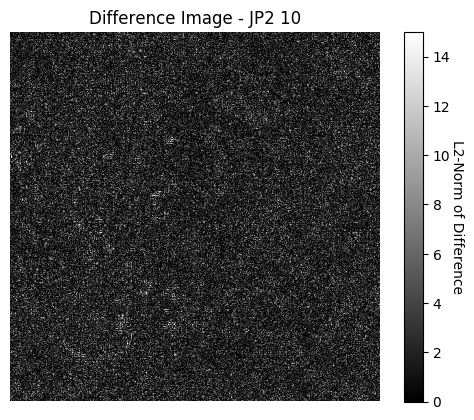
\includegraphics[width=\textwidth]{doc/thesis/0_figures/compare_quality/set1/jp2_10_center_diff_heatmap_rel.png}
            \caption{\gls{jp2} quality 10.}
            \label{fig:img_quality_center_heatmap_rel_10}
        \end{subfigure}
        \begin{subfigure}[b]{0.42\textwidth}
            \centering
            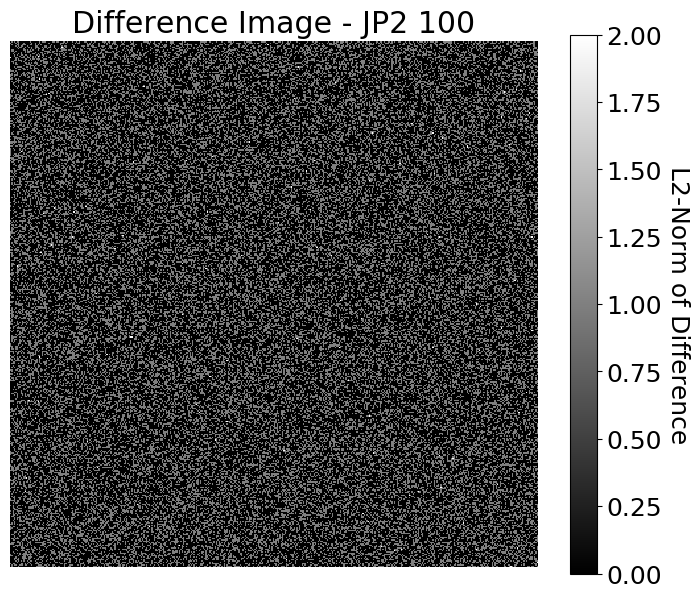
\includegraphics[width=\textwidth]{doc/thesis/0_figures/compare_quality/set1/jp2_100_center_diff_heatmap_rel.png}
            \caption{\gls{jp2} quality 100.}
            \label{fig:img_quality_center_heatmap_rel_100}
        \end{subfigure}
        \\
        \begin{subfigure}[b]{0.42\textwidth}
            \centering
            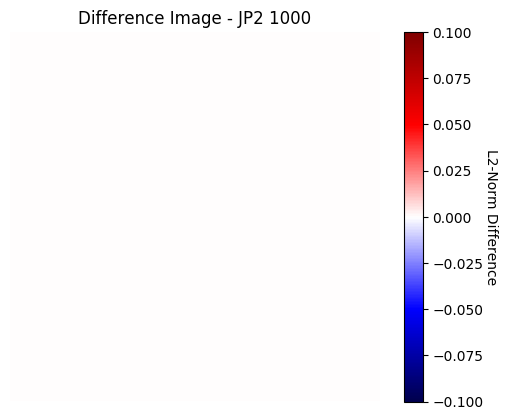
\includegraphics[width=\textwidth]{doc/thesis/0_figures/compare_quality/set1/jp2_1000_center_diff_heatmap_rel.png}
            \caption{\gls{jp2} quality 1000.}
            \label{fig:img_quality_center_heatmap_rel_1000}
        \end{subfigure}
        \begin{subfigure}[b]{0.42\textwidth}
            \centering
            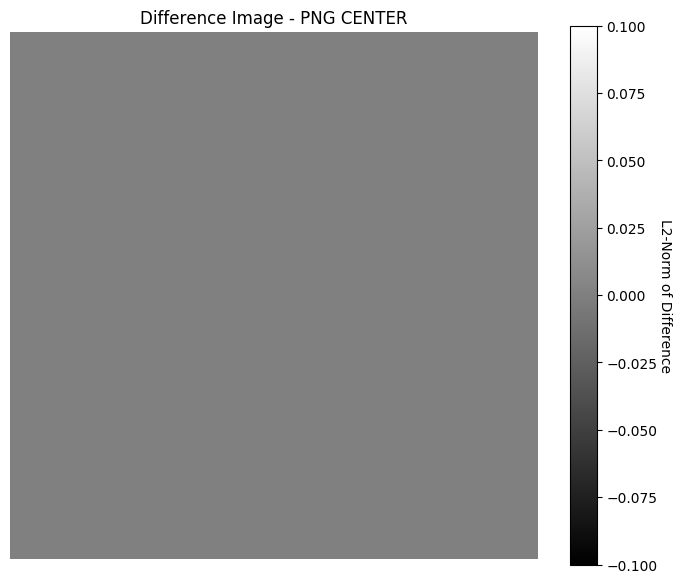
\includegraphics[width=\textwidth]{doc/thesis/0_figures/compare_quality/set1/png_center_diff_heatmap_rel.png}
            \caption{\gls{png}}
            \label{fig:img_quality_center_heatmap_rel_png}
        \end{subfigure}
    \caption{Difference images of close-ups with varying levels of compression using \gls{jp2} and one \gls{png} using different scales to show also smaller differences in the less compressed images. Image \ref{fig:img_quality_center_heatmap_rel_1000} is white because it does not differ from the \gls{png} image.}
    \label{fig:img_quality_center_heatmap_rel}
\end{figure}

\end{document}

%% Three levels of hierarchy in sectioning should be enough

%%\subsection*{Numerointi}
%%
%%Every section of the thesis begins on a new page. A subsection begins on a new 
%%page only if the previous page a full.
%%
%%The page numbering begins from the cover page and it is continuous through to 
%%the end. Arabian numerals are in the page numbering.
%%
%%The page numbers are made visibleafter the abstract pages, from the preface 
%%onwards, if there is one, or from the table of contents onwards.
%%
%%The list of references (bibliography) begins on a new page.
%%
%%Every appendix begins on a new page. Its page number continues from that on the
%%previous page.
%%
%%The page number is place on the upper corner of the page.

%% The example for embedding the graphics file linediagram.pdf into the document.
%% Command \inclugraphics[parametres]{argument} embeds the graphic.
%% Command \centering centres the graphic on the page horizontally. 
%% Command \caption numbers and places the caption at the position of occurrence.
%% Parameters htb force the figure to the current place of occurrence in the
%% source file, if there is sufficient space, or places it to the top or bottom
%% of the page. 
%\begin{figure}[htb]
%\centering
%% NOTE! The PDF/A-1b file created when using the jpg, pdf or png file below is
%% error-free. However, with kuva1.pdf, the resulting PDF/A-2b file fails the
%% compliance test in Acrobat Pro but passes it in PDF-XChanger and the validator
%% at https://www.pdf-online.com/osa/validate.aspx tarkistuksen.
%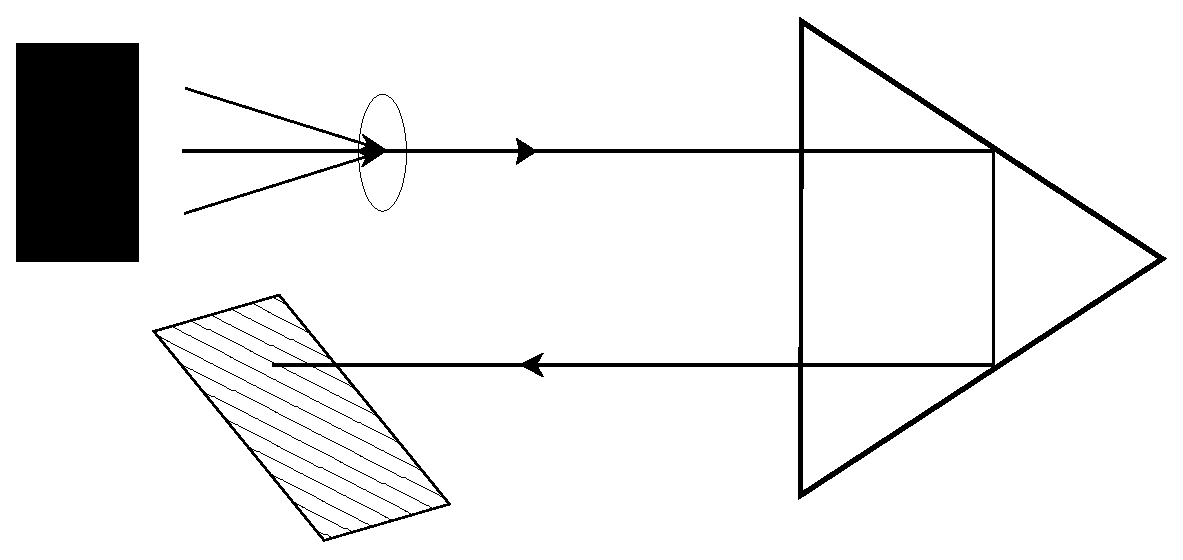
\includegraphics[height=5cm]{linediagram.eps}
%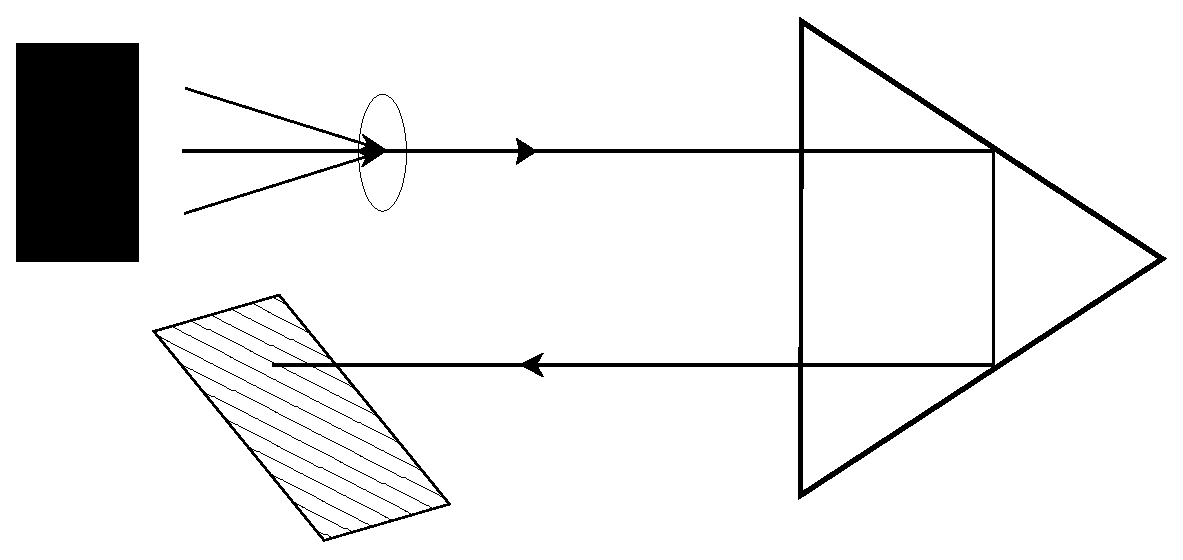
\includegraphics[height=5cm]{./linediagram.eps}
%\caption{This is an example of a numbered caption. \label{kuva1}}
%\end{figure}

% \begin{figure}[htb]
% \centering
% 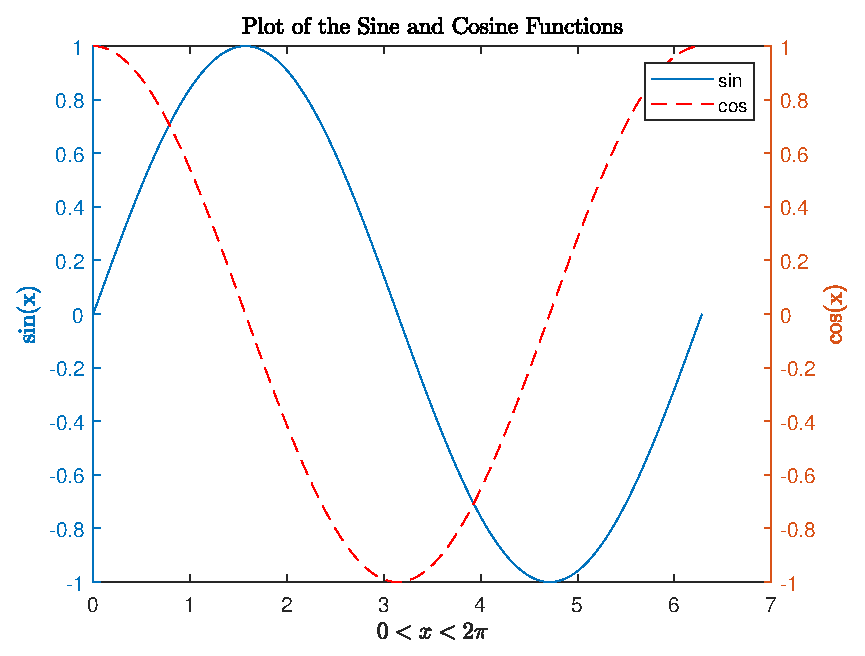
\includegraphics[height=5cm]{curves.eps}
% %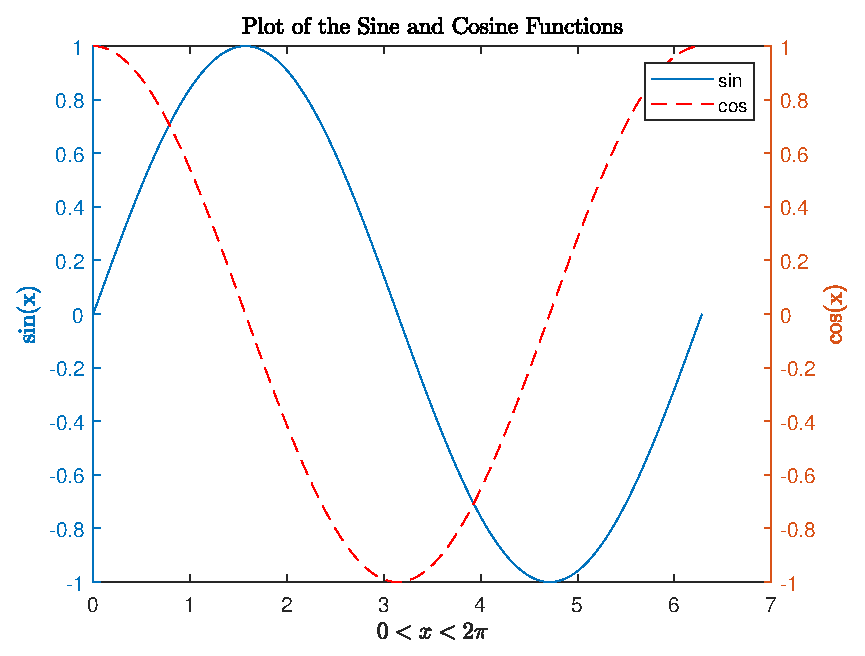
\includegraphics[height=5cm]{curves.eps}
% \caption{This is an example of a MATLAB graph. \label{kuva2}}
% \end{figure}